\documentclass[main.tex]{subfiles}

\begin{document}

\chapter{Cat Code Encoding}
For the cat code encoding, six simultaneous objectives were chosen to give encoding pulses which maps the six ``cardinal'' qubit states on the Bloch sphere to the corresponding cat code states in the resonator.
These initial qubit states are
\[ \ket{0}, \ket{1},\]
\[ \frac{\ket{0}+\ket{1}}{\sqrt{2}}, \frac{\ket{0}-\ket{1}}{\sqrt{2}},\]
\[ \frac{\ket{0}+i\ket{1}}{\sqrt{2}}, \frac{\ket{0}-i\ket{1}}{\sqrt{2}} \]
with target state \(\ket{0}\).
The resonator initial state is \(\ket{0}\) (in the Fock basis) and the corresponding target states are
\[ \cat{}, \cat[i]{},\]
\[ \frac{\cat{}+\cat[i]{}}{\sqrt{2}}, \frac{\cat{}-\cat[i]{}}{\sqrt{2}},\]
\[ \frac{\cat{}+i\cat[i]{}}{\sqrt{2}}, \frac{\cat{}-i\cat[i]{}}{\sqrt{2}}. \]
The hope is that by optimizing these six states simultaneously the pulse shapes will approximate the unitary in \Cref{eq:cat-code-unitary}.

\section{Simulation Setup}
In this section the Hamiltonian and the optimization parameters will be presented.

\subsection{Hamiltonian}
In this simulation the coupled qubit-resonator system in \Cref{eq:hamiltonian-coupled} was used.
As the operators \(\ad\) and \(\bd\) commute, the rewriting used in \Cref{eq:system-hamiltonian-rotating} was also used for the resonator.
The rotating frame transformation is done here with respect to \(\omega_{r} \au\ad + \omega_{q} \bu\bd \).
However, as the coupling term has no time dependence and does not commute with the operators \(\au\ad \) and \(\bu\bd \) there will still be a time dependence in the rotating frame
\begin{equation}
    g(\ad\bu + \au\bd) \rightarrow g(\ad\bu\ex^{i(\omega_q-\omega_r)t} + \au\bd\ex^{-i(\omega_q-\omega_r)t}).
    \label{eq:coupling-term-rotating}
\end{equation}
This was a problem because \krotov{} expects \(\Ham_d\) to be time independent.
There is a way to ``simulate'' the coupling term~\eqref{eq:coupling-term-rotating} by inserting it as an external time dependent pulse, and omitting it from optimization, which was done in this case.
The coupling term was then split into a real and imaginary part which is, as stated before, required by \krotov{}.

The final Hamiltonian provided to \krotov{} was then
\begin{equation}
    \begin{split}
        \Ham &= \underbrace{K_r/2(\au)^2\ad^2 +K_q/2\qty(\bu\bd)^2}_{\Ham_d} + \\
        &+\underbrace{\text{Re}\qty[\Omega_r(t)]}_{u_0(t)}\underbrace{(\ad + \au)}_{\Ham_0} + \underbrace{\text{Im}\qty[\Omega_r(t)]}_{u_1(t)}\underbrace{i(\ad - \au)}_{\Ham_1} + \underbrace{\text{Re}\qty[\Omega_q(t)]}_{u_2(t)}\underbrace{(\bd + \bu)}_{\Ham_2} + \underbrace{\text{Im}\qty[\Omega_q(t)]}_{u_3(t)}\underbrace{i(\bd - \bu)}_{\Ham_3} +\\
        &+\underbrace{\qty[\cos((\omega_q-\omega_r)t)]}_{u_4(t)}\underbrace{g(\ad\bu + \au\bd)}_{\Ham_4} + \underbrace{\qty[\sin((\omega_q-\omega_r)t)]}_{u_5(t)}\underbrace{ig(\ad\bu - \au\bd)}_{\Ham_5}
        \label{eq:cat-hamiltonian-rotating}
    \end{split}
\end{equation}
The parameters of this system are presented in \Cref{tab:ham-params}.
These were chosen to resemble the physical values measured in~\cite{ofek_extending_2016}, except for \(g\) which was chosen at relatively large value to reduce the pulse length needed to realise the transfer.
\begin{table}[H]
    \caption{Hamiltonian parameters}%
    \label{tab:ham-params}
    \centering
    \begin{tabular}{@{}ll@{}}
    \toprule
    Param. & Value\\ \midrule
    \(\omega_q/(2\pi)\) & \SI{6.2815}{\giga\hertz} \\
    \(K_q/(2\pi)\) & \SI{297}{\mega\hertz} \\
    \(\omega_r/(2\pi)\) & \SI{8.3056}{\giga\hertz} \\
    \(K_r/(2\pi)\) & \SI{4.5}{\kilo\hertz} \\
    \(g/(2\pi)\) & \SI{0.225}{\giga\hertz} \\
    \bottomrule
    \end{tabular}
\end{table}
The truncated Hilbert space size for the resonator was chosen to be \( N_r = 8 \) with the mean photon number \(\alpha = 2\).
Due to the large system size, the qubit's truncated Hilbert space size was set to \(N_q = 2\).

\subsection{Optimization Setup}
The optimization was setup in the same way as the previous simulation, however due to the rapid oscillations at \(|\omega_q-\omega_r|\) (due to the coupling pulse) a finer time discretization of \SI{24}{\giga\samples\per\second} was chosen.
The step size was chosen as \(\lambda = \frac{1}{\frac{1}{2}A_{m}}\) and the pulse length \(T = \ns{60}\) to allow the coupling to affect the system.
Further, convergence criteria was chosen as \(F>0.999999\) or \(\Delta F < \num{e-06}\).
Another important step in optimizing in the rotating frame was to convert the target states into the rotating frame in order for the final states to be correct in the lab frame.
Initial guess pulses were chosen to be the same Blackman pulses in the setup for the \(\ket{0}\rightarrow\ket{2}\) evolution.

\section{Results}
We now present the main results of this thesis: the optimization of pulses for encoding a cat state in a resonator from a coupled qubit.
The cat encoding optimization reached the convergence criteria of \(\Delta F < \num{e-6}\) after 2389 iterations (corresponding to roughly 41 hours and 28 minutes) with a fidelity \(F = 0.999234\), (recall the fidelity measure for multiple objectives in \Cref{eq:total-fidelity}).
The individual fidelities for the 6 initial states are shown in \Cref{tab:cat-fidelities}, where we can see that all individual fidelities are above 0.999000.

\begin{table}[ht]
    \caption{Fidelities for the individual state transfers (ordered from highest to lowest).}%
    \label{tab:cat-fidelities}
    \centering
    \begin{tabular}{@{}ll@{}}
    \toprule
    State & \(F\)\\ \midrule
	\((\ket{0}+i\ket{1})/\sqrt{2}\) & 0.99939453 \\
	\((\ket{0}-\ket{1})/\sqrt{2}\) & 0.99932348 \\
	\((\ket{0}+\ket{1})/\sqrt{2}\) & 0.99930147 \\
    \(\ket{0}\) & 0.99920509 \\
	\(\ket{1}\) & 0.99918837 \\
	\((\ket{0}-i\ket{1})/\sqrt{2}\) & 0.99899637 \\
    \bottomrule
    \end{tabular}
\end{table}

To corroborate how well the qubit was mapped to the cat code basis, multiple states spread around the Bloch sphere were transferred with the pulse solution.
The corresponding fidelities are shown on the Bloch sphere in \Cref{fig:bloch-fid}, where we can see an asymmetry with larger fidelities toward \((\ket{0}+i\ket{1})/\sqrt{2}\).
All in all the minimum fidelity among all the transferred states is 0.998996.

\begin{figure}[ht]
	\centering
	\subcaptionbox{Side view of Bloch sphere.}{
		\centering
		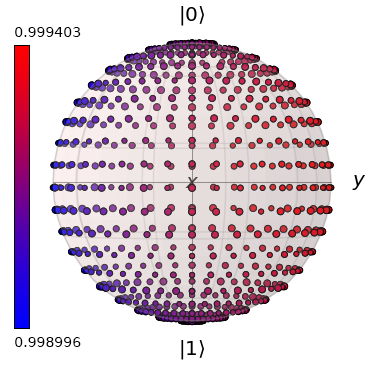
\includegraphics[width=0.45\textwidth]{figs/bloch_fid_low.png}
	}%
	\subcaptionbox{Top view of Bloch sphere.}{
		\centering
		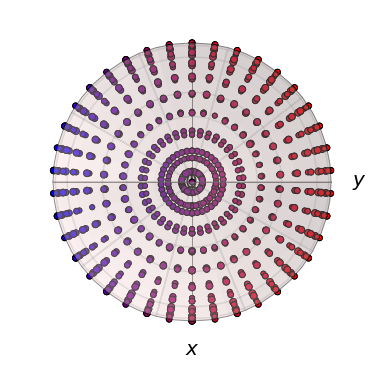
\includegraphics[width=0.45\textwidth]{figs/bloch_fid_high.png}
	}
	\caption{%
	The fidelities of every simulated state transfer shown on the Bloch sphere.
	There is an asymmetry in the fidelity with higher fidelity towards the state \((\ket{0}+i\ket{1})/\sqrt{2}\).
	}%
	\label{fig:bloch-fid}
\end{figure}


The pulse shapes of the qubit and resonator are shown in \Cref{fig:cat-pulse-shape}.
Comparing the resonator and qubit, we can see that the resonator pulse has rapid oscillations throughout the whole pulse while the qubit exhibits some small quick oscillation at sparse times.
The spectrum of the pulse is shown in \Cref{fig:cat-pulse-spectrum} and gives us some insight into the pulse shapes.
We can see that the qubit control pulse shows a wide peak at \(\omega_q\), two small peaks at \(\omega_r\) and \(2\omega_r-\omega_q\) and two barely noticeable peaks at \(\frac{1}{4}\omega_r\) and \(\frac{1}{2}\omega_r\). 
The resonator pulse has one wide peak at \(\omega_r\), a smaller one at \(\omega_q\) and an even smaller peak at \(2\omega_r-\omega_q\).

\begin{figure}[ht]
\centering
\subcaptionbox{Qubit control pulse shape.}{
		\centering
		\setlength\figureheight{20em}
		\setlength\figurewidth{\textwidth}
		% This file was created by matplotlib2tikz v0.7.4.
\begin{tikzpicture}

\definecolor{color0}{rgb}{0.12156862745098,0.466666666666667,0.705882352941177}
\definecolor{color1}{rgb}{1,0.498039215686275,0.0549019607843137}

\begin{axis}[
height=\figureheight,
legend cell align={left},
legend style={at={(0.03,0.97)}, anchor=north west, draw=white!80.0!black},
tick align=outside,
tick pos=left,
width=\figurewidth,
x grid style={white!69.01960784313725!black},
xlabel={Time (ns)},
xmin=-3, xmax=63,
xtick style={color=black},
y grid style={white!69.01960784313725!black},
ymin=-0.218166156499413, ymax=0.218166156499413,
ytick style={color=black}
]
\addplot [semithick, color0]
table {%
0 0
0.0416956219596942 3.08728176247894e-05
0.0833912439193885 0.000102118495005609
0.125086865879083 0.000202653307067725
0.166782487838777 0.000391795170413738
0.208478109798471 0.000723296826254682
0.250173731758165 0.00119484646234114
0.29186935371786 0.00171555495194023
0.333564975677554 0.0022560307507813
0.375260597637248 0.00303026439470639
0.416956219596942 0.00406074506641338
0.458651841556637 0.00524658729310708
0.500347463516331 0.00603705064836644
0.542043085476025 0.0061422152747051
0.583738707435719 0.00600568336127842
0.625434329395413 0.00628574631016776
0.667129951355108 0.00772560801819381
0.708825573314802 0.00984687116549382
0.750521195274496 0.011852567770109
0.79221681723419 0.0134501293843006
0.833912439193885 0.0148922880960751
0.875608061153579 0.0173724084956246
0.917303683113273 0.0204166049304492
0.958999305072967 0.0229402681707778
1.00069492703266 0.0235645417094428
1.04239054899236 0.0222063057343637
1.08408617095205 0.0212344751634797
1.12578179291174 0.0220860569485837
1.16747741487144 0.0254083030472539
1.20917303683113 0.0292722292285361
1.25086865879083 0.0317728595087875
1.29256428075052 0.0334387762339531
1.33425990271022 0.0352550832639918
1.37595552466991 0.0390486222496993
1.4176511466296 0.043283322936511
1.4593467685893 0.0455162203489598
1.50104239054899 0.0447527917837088
1.54273801250869 0.0418524722713003
1.58443363446838 0.0408712982266991
1.62612925642807 0.0428956434548439
1.66782487838777 0.0470584884094371
1.70952050034746 0.0504975563913077
1.75121612230716 0.051134653746733
1.79291174426685 0.0510223234886867
1.83460736622655 0.0517730079651744
1.87630298818624 0.0547205235218682
1.91799861014593 0.0577437826633267
1.95969423210563 0.0579027283890363
2.00138985406532 0.0555486359147569
2.04308547602502 0.0523458666646414
2.08478109798471 0.0520652426863471
2.12647671994441 0.0546412135166845
2.1681723419041 0.0576593321190783
2.20986796386379 0.0587475659286213
2.25156358582349 0.0567404588921621
2.29325920778318 0.0546218214800052
2.33495482974288 0.0541642818599181
2.37665045170257 0.0556932061209978
2.41834607366227 0.0572305936700594
2.46004169562196 0.0561969738522291
2.50173731758165 0.0538719437220971
2.54343293954135 0.0520239612567465
2.58512856150104 0.0530689188630793
2.62682418346074 0.0560594058270375
2.66851980542043 0.0577857369547568
2.71021542738012 0.056784900507561
2.75191104933982 0.0529835890444149
2.79360667129951 0.0497107379288607
2.83530229325921 0.0486484979442381
2.8769979152189 0.0491067596995916
2.9186935371786 0.0493241712053322
2.96038915913829 0.0473073031477836
3.00208478109798 0.0449611515086254
3.04378040305768 0.0441040193217554
3.08547602501737 0.0457156877440102
3.12717164697707 0.0481796387519173
3.16886726893676 0.0480181636343069
3.21056289089646 0.0448536408877749
3.25225851285615 0.0397692245198964
3.29395413481584 0.0359591984500161
3.33564975677554 0.0346678579623335
3.37734537873523 0.0341659739250372
3.41904100069493 0.0329970055426267
3.46073662265462 0.0300574550676464
3.50243224461432 0.0276357485738356
3.54412786657401 0.0274050941928904
3.5858234885337 0.0287983017043148
3.6275191104934 0.0298243007928736
3.66921473245309 0.0274308879605148
3.71091035441279 0.0224941196889132
3.75260597637248 0.0171194289376849
3.79430159833217 0.0136751681371585
3.83599722029187 0.0125467317258969
3.87769284225156 0.0111457045800248
3.91938846421126 0.00860060533255531
3.96108408617095 0.00503001104102974
4.00277970813065 0.00267225850110856
4.04447533009034 0.00269318842587986
4.08617095205003 0.0030191255055853
4.12786657400973 0.00183457144964909
4.16956219596942 -0.00260702285095254
4.21125781792912 -0.00826332710894012
4.25295343988881 -0.0125398768680729
4.29464906184851 -0.0147448739172678
4.3363446838082 -0.0155748864765715
4.37804030576789 -0.0178253320187945
4.41973592772759 -0.0214051090423912
4.46143154968728 -0.0248909193152492
4.50312717164698 -0.0269128065963184
4.54482279360667 -0.0272175522621949
4.58651841556637 -0.0288370349323765
4.62821403752606 -0.0325620530895859
4.66990965948575 -0.0380196670823566
4.71160528144545 -0.0427017439904221
4.75330090340514 -0.0445094851793406
4.79499652536484 -0.0450276871538617
4.83669214732453 -0.0457308613270513
4.87838776928422 -0.0484567872632656
4.92008339124392 -0.0521015461475833
4.96177901320361 -0.0544754858428665
5.00347463516331 -0.056103948011982
5.045170257123 -0.0577012647225187
5.0868658790827 -0.0618721734167146
5.12856150104239 -0.0675550509807796
5.17025712300208 -0.072065906280364
5.21195274496178 -0.0738754348004555
5.25364836692147 -0.0725085565827191
5.29534398888117 -0.0715081691205152
5.33703961084086 -0.0722159911943362
5.37873523280056 -0.0743031468578437
5.42043085476025 -0.0764555423660723
5.46212647671994 -0.0769761489053115
5.50382209867964 -0.0787933462486016
5.54551772063933 -0.0828664670307023
5.58721334259903 -0.0893274984043596
5.62890896455872 -0.0951476898591123
5.67060458651842 -0.0963194286048575
5.71230020847811 -0.0939986446240948
5.7539958304378 -0.0899297310387777
5.7956914523975 -0.087924038336494
5.83738707435719 -0.0881249142964814
5.87908269631689 -0.0877058533148682
5.92077831827658 -0.0868806163287618
5.96247394023627 -0.0859043687469862
6.00416956219597 -0.0891555842970442
6.04586518415566 -0.0963624464921563
6.08756080611536 -0.103459860973945
6.12925642807505 -0.106679649456319
6.17095205003475 -0.102849859692709
6.21264767199444 -0.0966440855907125
6.25434329395413 -0.0914210623965095
6.29603891591383 -0.0885889850293319
6.33773453787352 -0.0867726122367871
6.37943015983322 -0.0819810239665612
6.42112578179291 -0.0778093350289609
6.46282140375261 -0.0770939198749902
6.5045170257123 -0.0829541032638226
6.54621264767199 -0.0924549598837529
6.58790826963169 -0.0973336532919551
6.62960389159138 -0.0955125527425308
6.67129951355108 -0.0870446434506875
6.71299513551077 -0.078908158913635
6.75469075747047 -0.074231938055964
6.79638637943016 -0.0698024697654205
6.83808200138985 -0.0638799646438942
6.87977762334955 -0.0541329118726888
6.92147324530924 -0.0480066565466894
6.96316886726894 -0.0499099799815595
7.00486448922863 -0.0582996642653317
7.04656011118832 -0.0674158209389297
7.08825573314802 -0.0673068243432482
7.12995135510771 -0.0599480406948878
7.17164697706741 -0.0497001568174606
7.2133425990271 -0.0424188956208292
7.2550382209868 -0.0388650116814018
7.29673384294649 -0.0312498921572847
7.33842946490618 -0.0198313459882228
7.38012508686588 -0.00681140116379316
7.42182070882557 -0.00144097320092356
7.46351633078527 -0.00730708165934519
7.50521195274496 -0.0162732756089583
7.54690757470466 -0.0215379674701229
7.58860319666435 -0.0157233707905019
7.63029881862404 -0.00528898612706804
7.67199444058374 0.00244330582805082
7.71369006254343 0.00681977324157735
7.75538568450313 0.0103653471753768
7.79708130646282 0.0223083263889337
7.83877692842252 0.0383668186504852
7.88047255038221 0.0508891717388114
7.9221681723419 0.0528851473959427
7.9638637943016 0.0439460162895669
8.00555941626129 0.037336320513646
8.04725503822099 0.0379228961919574
8.08895066018068 0.0468216559004181
8.13064628214038 0.0556221610140595
8.17234190410007 0.0574338453215871
8.21403752605976 0.0586789942475068
8.25573314801946 0.0639593016309458
8.29742876997915 0.0791322531973288
8.33912439193885 0.0960986873871865
8.38082001389854 0.103888137509771
8.42251563585823 0.101437545740464
8.46421125781793 0.09217397606998
8.50590687977762 0.0897360528243063
8.54760250173732 0.0948990428321957
8.58929812369701 0.101984294499531
8.63099374565671 0.104825632320164
8.6726893676164 0.100249669967594
8.71438498957609 0.0994556411616443
8.75608061153579 0.106626413919568
8.79777623349548 0.12106221143422
8.83947185545518 0.133680755785695
8.88116747741487 0.134307705872803
8.92286309937457 0.12830723345937
8.96455872133426 0.121424069138408
9.00625434329395 0.122467743868105
9.04794996525365 0.128421848222505
9.08964558721334 0.129922570319749
9.13134120917304 0.12561266918386
9.17303683113273 0.116877641933404
9.21473245309242 0.114666780520714
9.25642807505212 0.121098266189858
9.29812369701181 0.129812811618193
9.33981931897151 0.134195486523509
9.3815149409312 0.128274199348465
9.4232105628909 0.120702180812316
9.46490618485059 0.117139393616388
9.50660180681028 0.119528473693942
9.54829742876998 0.123198798543586
9.58999305072967 0.11924013852412
9.63168867268937 0.109923254650924
9.67338429464906 0.0995080505416918
9.71507991660875 0.0950648643009518
9.75677553856845 0.0970236319088336
9.79847116052814 0.0973535136630077
9.84016678248784 0.0932394206431243
9.88186240444753 0.0835794156136412
9.92355802640723 0.0762777007771278
9.96525364836692 0.0754908157293361
10.0069492703266 0.0783097294466375
10.0486448922863 0.0798890586978153
10.090340514246 0.0737092697401794
10.1320361362057 0.0625130559689619
10.1737317581654 0.0514152603438583
10.2154273801251 0.0439328769165515
10.2571230020848 0.0400272315271376
10.2988186240445 0.0334802818553019
10.3405142460042 0.0238897396790746
10.3822098679639 0.0134588406676115
10.4239054899236 0.00790613644847617
10.4656011118833 0.00986560420669541
10.5072967338429 0.014702666707186
10.5489923558026 0.016821485099044
10.5906879777623 0.0114675544083408
10.632383599722 0.00052821530961567
10.6740792216817 -0.0107019806612064
10.7157748436414 -0.0196926995575379
10.7574704656011 -0.0269105779457357
10.7991660875608 -0.0363152484811951
10.8408617095205 -0.0476183592556221
10.8825573314802 -0.0568069105813237
10.9242529534399 -0.0588016576043848
10.9659485753996 -0.052552859013746
11.0076441973593 -0.0435634017907737
11.049339819319 -0.0391016196480738
11.0910354412787 -0.0428968391290806
11.1327310632384 -0.0521263958121794
11.1744266851981 -0.0613196859105004
11.2161223071577 -0.0679786777219634
11.2578179291174 -0.074349781427894
11.2995135510771 -0.0836317809382477
11.3412091730368 -0.094227409843642
11.3829047949965 -0.100563107812084
11.4246004169562 -0.0970258431466527
11.4662960389159 -0.0852557655578433
11.5079916608756 -0.0727640053632801
11.5496872828353 -0.0670619419706814
11.591382904795 -0.0699015561753328
11.6330785267547 -0.0753801034483817
11.6747741487144 -0.0789153180329307
11.7164697706741 -0.0802456450516521
11.7581653926338 -0.0839571928751105
11.7998610145935 -0.0927493489973825
11.8415566365532 -0.101443610631646
11.8832522585129 -0.103234519956923
11.9249478804725 -0.093925061302618
11.9666435024322 -0.0786856477740102
12.0083391243919 -0.0669786553868318
12.0500347463516 -0.0627918186119934
12.0917303683113 -0.0642972668040507
12.133425990271 -0.0637003433134107
12.1751216122307 -0.0596258509344054
12.2168172341904 -0.0566434668850845
12.2585128561501 -0.0594555603678318
12.3002084781098 -0.0682104102263091
12.3419041000695 -0.0739189780854235
12.3835997220292 -0.0705026075520486
12.4252953439889 -0.0586563490347585
12.4669909659486 -0.0455739427712431
12.5086865879083 -0.0395054678717801
12.550382209868 -0.0381383964169072
12.5920778318277 -0.0364081139930239
12.6337734537874 -0.0294236102254481
12.675469075747 -0.0203780756380819
12.7171646977067 -0.017452032408657
12.7588603196664 -0.021792070419204
12.8005559416261 -0.0292875540413422
12.8422515635858 -0.0310618368031218
12.8839471855455 -0.0244985548778284
12.9256428075052 -0.0158065685871154
12.9673384294649 -0.0103632895490887
13.0090340514246 -0.0108899582881951
13.0507296733843 -0.0105374102952383
13.092425295344 -0.00433552483058609
13.1341209173037 0.00577485238684786
13.1758165392634 0.0139239066912802
13.2175121612231 0.0136522673759917
13.2592077831828 0.00846047967847482
13.3009034051425 0.0049141805778436
13.3425990271022 0.00651867243549132
13.3842946490618 0.0116370587316899
13.4259902710215 0.0130399250040902
13.4676858929812 0.0103737434516439
13.5093815149409 0.00744070485696881
13.5510771369006 0.00982523839003874
13.5927727588603 0.0185882525996982
13.63446838082 0.0268873555169654
13.6761640027797 0.0303609208540934
13.7178596247394 0.028691510160628
13.7595552466991 0.0264808742498659
13.8012508686588 0.0279656830730906
13.8429464906185 0.0301599183524116
13.8846421125782 0.0298285259195243
13.9263377345379 0.0250720569531213
13.9680333564976 0.0197327185133677
14.0097289784573 0.0196130371312246
14.051424600417 0.0245585421171248
14.0931202223766 0.03138227578281
14.1348158443363 0.0353778793548299
14.176511466296 0.0362480152767484
14.2182070882557 0.0381963541685928
14.2599027102154 0.0417211863132587
14.3015983321751 0.0452966926973031
14.3432939541348 0.044662741949707
14.3849895760945 0.039127771031179
14.4266851980542 0.0338940119579592
14.4683808200139 0.0322714520163161
14.5100764419736 0.0355247087979719
14.5517720639333 0.0396092492110091
14.593467685893 0.0411240591069713
14.6351633078527 0.0429680544320714
14.6768589298124 0.0470725451223177
14.7185545517721 0.0551195494345929
14.7602501737318 0.0620497722743225
14.8019457956915 0.0623542154414539
14.8436414176511 0.0577849190299655
14.8853370396108 0.0518437841786268
14.9270326615705 0.0511539335196587
14.9687282835302 0.0542094306549683
15.0104239054899 0.0554774634972116
15.0521195274496 0.054196907133908
15.0938151494093 0.0516489038300129
15.135510771369 0.0561624168729144
15.1772063933287 0.0670470214835351
15.2189020152884 0.0773365030910495
15.2605976372481 0.0811250827260245
15.3022932592078 0.0751333559009729
15.3439888811675 0.0692675895592299
15.3856845031272 0.068361870901353
15.4273801250869 0.0716012162819995
15.4690757470466 0.0733287936653875
15.5107713690063 0.0661887827096901
15.5524669909659 0.058712377113391
15.5941626129256 0.0577801500071715
15.6358582348853 0.0678299710450457
15.677553856845 0.0822782707720713
15.7192494788047 0.0868393284568017
15.7609451007644 0.0823006601154829
15.8026407227241 0.0730505003191667
15.8443363446838 0.0707345134336385
15.8860319666435 0.0761488855743543
15.9277275886032 0.0769588389291113
15.9694232105629 0.0694218852279108
16.0111188325226 0.0532059945308701
16.0528144544823 0.044424098751627
16.094510076442 0.0506629362301418
16.1362056984017 0.0635678286595045
16.1779013203614 0.0729920536920257
16.2195969423211 0.0667190479738456
16.2612925642808 0.055754172583639
16.3029881862404 0.0513551699122495
16.3446838082001 0.0557883535890428
16.3863794301598 0.0625953728530886
16.4280750521195 0.0538196137790201
16.4697706740792 0.03467485956998
16.5114662960389 0.0168870569115097
16.5531619179986 0.0140198484139589
16.5948575399583 0.0272507180042755
16.636553161918 0.0358590253927162
16.6782487838777 0.0333324028668887
16.7199444058374 0.0198944755292966
16.7616400277971 0.0115835101167597
16.8033356497568 0.018699431818697
16.8450312717165 0.0274797932823486
16.8867268936762 0.0271912065078586
16.9284225156359 0.00737793880629371
16.9701181375956 -0.0165099254902628
17.0118137595552 -0.0253122745113621
17.0535093815149 -0.0191842224425719
17.0952050034746 -0.00611360233344936
17.1369006254343 -0.00778118839601469
17.178596247394 -0.0208671674559323
17.2202918693537 -0.0306893270439171
17.2619874913134 -0.0275332323799039
17.3036831132731 -0.0109273677068354
17.3453787352328 -0.00540777727519124
17.3870743571925 -0.017869803461728
17.4287699791522 -0.04159060546447
17.4704656011119 -0.0584826456246915
17.5121612230716 -0.053641398836064
17.5538568450313 -0.0431942821098231
17.595552466991 -0.0394273598278611
17.6372480889507 -0.0509669217763576
17.6789437109104 -0.0653379784160347
17.72063933287 -0.0625133671194667
17.7623349548297 -0.0477076313162087
17.8040305767894 -0.0319674444521134
17.8457261987491 -0.0359732029244502
17.8874218207088 -0.0566252474724179
17.9291174426685 -0.0729911974700523
17.9708130646282 -0.0756223786011462
18.0125086865879 -0.062845412505715
18.0542043085476 -0.0572322405246234
18.0958999305073 -0.0665154869189286
18.137595552467 -0.0808534518320778
18.1792911744267 -0.0865260933648842
18.2209867963864 -0.0713240895014073
18.2626824183461 -0.0535407377435455
18.3043780403058 -0.0483083924786531
18.3460736622655 -0.0602316411469549
18.3877692842252 -0.0781670440268954
18.4294649061848 -0.0802753944238933
18.4711605281445 -0.0713418734289804
18.5128561501042 -0.0618044836169469
18.5545517720639 -0.066652576143796
18.5962473940236 -0.0837344806144808
18.6379430159833 -0.0920655712495801
18.679638637943 -0.0857509243441629
18.7213342599027 -0.0667847009974095
18.7630298818624 -0.0553326065910891
18.8047255038221 -0.0609375113858782
18.8464211257818 -0.0720093402067064
18.8881167477415 -0.0777005300845903
18.9298123697012 -0.0675423449572089
18.9715079916609 -0.0560962867452493
19.0132036136206 -0.0567029283063393
19.0548992355803 -0.0691055013127541
19.09659485754 -0.0838772759293969
19.1382904794997 -0.0822465388689925
19.1799861014593 -0.0687492693534832
19.221681723419 -0.0550228893087627
19.2633773453787 -0.051975164703923
19.3050729673384 -0.0600662557398883
19.3467685892981 -0.0618493485418574
19.3884642112578 -0.0538572418715765
19.4301598332175 -0.0393324695859977
19.4718554551772 -0.0325678732147609
19.5135510771369 -0.0413188666257583
19.5552466990966 -0.0535237384407053
19.5969423210563 -0.0596781059113062
19.638637943016 -0.0514780224039479
19.6803335649757 -0.038580582316726
19.7220291869354 -0.0330332948038724
19.7637248088951 -0.0338165390719967
19.8054204308548 -0.0361732253449586
19.8471160528145 -0.0275180806724713
19.8888116747741 -0.0120608809277963
19.9305072967338 -0.00047723960478926
19.9722029186935 0.000221543600682913
20.0138985406532 -0.0106038495200833
20.0555941626129 -0.0182395650474335
20.0972897845726 -0.017583688225306
20.1389854065323 -0.00977018620973709
20.180681028492 -0.00252753136019598
20.2223766504517 -0.00300926567148395
20.2640722724114 -0.00332061378132338
20.3057678943711 0.00125319038564732
20.3474635163308 0.0146768745259982
20.3891591382905 0.0296392921642267
20.4308547602502 0.0349991928002983
20.4725503822099 0.0311124200316356
20.5142460041696 0.0212735427261414
20.5559416261293 0.0164793195741303
20.597637248089 0.0181515621869693
20.6393328700486 0.02080823612973
20.6810284920083 0.021440575406005
20.722724113968 0.0176926966029098
20.7644197359277 0.0182364623549105
20.8061153578874 0.0257718673370252
20.8478109798471 0.0375560513155726
20.8895066018068 0.0471096561582916
20.9312022237665 0.0460407945923384
20.9728978457262 0.0386150868017064
21.0145934676859 0.0294879486654589
21.0562890896456 0.0246036964939137
21.0979847116053 0.0239378142055234
21.139680333565 0.0211742156202928
21.1813759555247 0.0167755027092717
21.2230715774844 0.0115421014285866
21.2647671994441 0.0117886647234536
21.3064628214038 0.0186286947277794
21.3481584433634 0.0257733407181669
21.3898540653231 0.0287731430073919
21.4315496872828 0.0228201236180017
21.4732453092425 0.0132943618828474
21.5149409312022 0.00532773608946713
21.5566365531619 0.000546394479606108
21.5983321751216 -0.00187461434451451
21.6400277970813 -0.00758674778584481
21.681723419041 -0.0145424292567349
21.7234190410007 -0.0197459388346147
21.7651146629604 -0.0198648212026464
21.8068102849201 -0.0148975076486271
21.8485059068798 -0.0121776895938036
21.8902015288395 -0.0142545494326959
21.9318971507992 -0.022083305238084
21.9735927727589 -0.0305702673402949
22.0152883947186 -0.0350711126774914
22.0569840166782 -0.0376484108992501
22.0986796386379 -0.0401869152268092
22.1403752605976 -0.0465020626989927
22.1820708825573 -0.0537200739242127
22.223766504517 -0.0573448162797853
22.2654621264767 -0.0568340156552407
22.3071577484364 -0.0533972956957743
22.3488533703961 -0.0535303008098026
22.3905489923558 -0.0578786444125629
22.4322446143155 -0.0637495845543129
22.4739402362752 -0.0675862029337359
22.5156358582349 -0.0668960052646182
22.5573314801946 -0.0666247028396083
22.5990271021543 -0.0690968331130435
22.640722724114 -0.0747965973805353
22.6824183460737 -0.0803071618357383
22.7241139680334 -0.0809944062811171
22.765809589993 -0.079070624261741
22.8075052119527 -0.0768970128946452
22.8492008339124 -0.078127993799207
22.8908964558721 -0.0813921641575436
22.9325920778318 -0.0817753479496607
22.9742876997915 -0.0790958274636793
23.0159833217512 -0.074317261132521
23.0576789437109 -0.072938516210295
23.0993745656706 -0.0759834269266243
23.1410701876303 -0.0797783469283268
23.18276580959 -0.0817143748837015
23.2244614315497 -0.079296092769677
23.2661570535094 -0.0766622054819967
23.3078526754691 -0.0760216557752204
23.3495482974288 -0.0760515817714016
23.3912439193885 -0.0745293684424239
23.4329395413482 -0.0676689697158352
23.4746351633079 -0.0597414327938902
23.5163307852675 -0.0545101757854513
23.5580264072272 -0.053970755558039
23.5997220291869 -0.0567277206419556
23.6414176511466 -0.0568515877009262
23.6831132731063 -0.0548342016127463
23.724808895066 -0.0518922703708457
23.7665045170257 -0.0505260725982718
23.8082001389854 -0.0505739575663973
23.8498957609451 -0.0460040388629551
23.8915913829048 -0.0369378967294293
23.9332870048645 -0.0247515421345726
23.9749826268242 -0.0158171937864041
24.0166782487839 -0.0135848604701689
24.0583738707436 -0.0136501454095137
24.1000694927033 -0.0137368614482428
24.141765114663 -0.0106059946774415
24.1834607366227 -0.00793288003429871
24.2251563585823 -0.00883309962478831
24.266851980542 -0.00930141612528749
24.3085476025017 -0.0063996649437621
24.3502432244614 0.00534533971693628
24.3919388464211 0.0206662441434594
24.4336344683808 0.032169943895051
24.4753300903405 0.0372760697270292
24.5170257123002 0.03620200082594
24.5587213342599 0.0372518783060062
24.6004169562196 0.0401650179280829
24.6421125781793 0.041599336508634
24.683808200139 0.0393316448649034
24.7255038220987 0.0331304392092015
24.7671994440584 0.0338374494889116
24.8088950660181 0.0437883717799035
24.8505906879778 0.0605461048717822
24.8922863099375 0.0754487570284931
24.9339819318972 0.0798564770712092
24.9756775538568 0.0793328017768544
25.0173731758165 0.0777260132365346
25.0590687977762 0.0796124846748973
25.1007644197359 0.0809714989222152
25.1424600416956 0.0741420327948978
25.1841556636553 0.0643644884053763
25.225851285615 0.0571917180762597
25.2675469075747 0.063006146433495
25.3092425295344 0.079227751283383
25.3509381514941 0.0936339008237669
25.3926337734538 0.100476765676211
25.4343293954135 0.0966544457005722
25.4760250173732 0.0929020032578032
25.5177206393329 0.0927550379870521
25.5594162612926 0.0912596788577094
25.6011118832523 0.0842485138649691
25.642807505212 0.0673404551939603
25.6845031271716 0.0536618363122675
25.7261987491313 0.0518746087504482
25.767894371091 0.0627405968012726
25.8095899930507 0.0786179359638101
25.8512856150104 0.084248634356537
25.8929812369701 0.0814447182508805
25.9346768589298 0.0747548608719028
25.9763724808895 0.0712949262759132
26.0180681028492 0.0705910216038892
26.0597637248089 0.0608579849732079
26.1014593467686 0.0431142983571295
26.1431549687283 0.0220466566310774
26.184850590688 0.0115922499581469
26.2265462126477 0.0177496941673668
26.2682418346074 0.0297789567912645
26.3099374565671 0.0393212363330939
26.3516330785268 0.0373824117200691
26.3933287004864 0.0311043951196926
26.4350243224461 0.0283371606287189
26.4767199444058 0.0266636709672252
26.5184155663655 0.0219800685463151
26.5601111883252 0.00476565409988181
26.6018068102849 -0.0175748040868175
26.6435024322446 -0.0329056801098
26.6851980542043 -0.0344748392412339
26.726893676164 -0.0224253286677797
26.7685892981237 -0.0119951700649587
26.8102849200834 -0.00822532720633734
26.8519805420431 -0.01021443119609
26.8936761640028 -0.0116103888587377
26.9353717859625 -0.00735438663634196
26.9770674079222 -0.0069441138557355
27.0187630298819 -0.0149730613697181
27.0604586518416 -0.0321240372002089
27.1021542738012 -0.0485202432966074
27.1438498957609 -0.0515711056405423
27.1855455177206 -0.0434308301157278
27.2272411396803 -0.0295959010918238
27.26893676164 -0.0210406278122402
27.3106323835997 -0.0184596332245051
27.3523280055594 -0.0145341299620708
27.3940236275191 -0.00720596921550766
27.4357192494788 0.00268188917987777
27.4774148714385 0.00542807219416762
27.5191104933982 -0.00153168525837963
27.5608061153579 -0.0111178205094375
27.6025017373176 -0.0155497554673428
27.6441973592773 -0.00815721364781851
27.685892981237 0.00423274145495588
27.7275886031967 0.0144426885092354
27.7692842251564 0.019717041093587
27.8109798471161 0.0230959929238783
27.8526754690757 0.0319254493480406
27.8943710910354 0.0445940146961241
27.9360667129951 0.0554528216239258
27.9777623349548 0.0592770379669622
28.0194579569145 0.0563100275410186
28.0611535788742 0.0549906503273671
28.1028492008339 0.0590311537797943
28.1445448227936 0.0676422193551181
28.1862404447533 0.0747142332116166
28.227936066713 0.0759296000368047
28.2696316886727 0.0746301622828207
28.3113273106324 0.0760920719958329
28.3530229325921 0.0832976506780617
28.3947185545518 0.093440057258786
28.4364141765115 0.100213238082656
28.4781097984712 0.102369965304794
28.5198054204309 0.102024534026375
28.5615010423905 0.10318283659042
28.6031966643502 0.106407827611349
28.6448922863099 0.107447347191637
28.6865879082696 0.103107568788533
28.7282835302293 0.0940139846892928
28.769979152189 0.0843123380427474
28.8116747741487 0.0796064788525178
28.8533703961084 0.0795684681491768
28.8950660180681 0.0818267553728354
28.9367616400278 0.0829013888880112
28.9784572619875 0.081570912482555
29.0201528839472 0.0803222877686258
29.0618485059069 0.0789287880985718
29.1035441278666 0.0764179176875077
29.1452397498263 0.0699042378625059
29.186935371786 0.0566855113800522
29.2286309937457 0.040442329662138
29.2703266157054 0.0240224327053272
29.312022237665 0.0124437379730527
29.3537178596247 0.00632792478881666
29.3954134815844 0.00250450681847792
29.4371091035441 0.000201684961071588
29.4788047255038 -0.00313855970314979
29.5205003474635 -0.00535111466494706
29.5621959694232 -0.00652291867833941
29.6038915913829 -0.0101145076096448
29.6455872133426 -0.0174524818588649
29.6872828353023 -0.0326203199625178
29.728978457262 -0.051161635993307
29.7706740792217 -0.0682706267879279
29.8123697011814 -0.0807103105409325
29.8540653231411 -0.0861199073051563
29.8957609451008 -0.0898291070877803
29.9374565670605 -0.0916087818266692
29.9791521890202 -0.0917883826004805
30.0208478109798 -0.0896016583278733
30.0625434329395 -0.0839580483467556
30.1042390548992 -0.0821644713014873
30.1459346768589 -0.0861055429322196
30.1876302988186 -0.0974389466957887
30.2293259207783 -0.111657277821967
30.271021542738 -0.120738604840498
30.3127171646977 -0.125509174357481
30.3544127866574 -0.125103398456287
30.3961084086171 -0.124119325687889
30.4378040305768 -0.122100873314591
30.4794996525365 -0.115141508309157
30.5211952744962 -0.105427395440492
30.5628908964559 -0.0936479883066817
30.6045865184156 -0.0874118271719199
30.6462821403753 -0.0885708120794123
30.687977762335 -0.0923743884112347
30.7296733842946 -0.0957676239353587
30.7713690062543 -0.0925281371450156
30.813064628214 -0.0871696701898785
30.8547602501737 -0.0818221953518921
30.8964558721334 -0.0764521878120172
30.9381514940931 -0.0707409279750354
30.9798471160528 -0.0600414979481876
31.0215427380125 -0.0485341904341672
31.0632383599722 -0.0395082988181425
31.1049339819319 -0.0349011771870608
31.1466296038916 -0.0345959459224006
31.1883252258513 -0.030683733038385
31.230020847811 -0.0233370048034063
31.2717164697707 -0.012723531702698
31.3134120917304 -0.00294368230874526
31.3551077136901 0.00302135999701855
31.3968033356498 0.00882322508500182
31.4384989576094 0.0141350137843878
31.4801945795691 0.0199117002710886
31.5218902015288 0.0236900418501953
31.5635858234885 0.0229116170886452
31.6052814454482 0.0221970549176969
31.6469770674079 0.0233277532107587
31.6886726893676 0.0302179848369043
31.7303683113273 0.0404628610924251
31.772063933287 0.0498420847719028
31.8137595552467 0.057657456233666
31.8554551772064 0.0621590322310098
31.8971507991661 0.0649521035963466
31.9388464211258 0.0649009497654317
31.9805420430855 0.0599699855008521
32.0222376650452 0.0523198686353368
32.0639332870049 0.0434598974969292
32.1056289089646 0.038543364320239
32.1473245309243 0.0386873013834412
32.1890201528839 0.0423285618563485
32.2307157748436 0.048461225387502
32.2724113968033 0.0548716809511482
32.314107018763 0.0613754585038115
32.3558026407227 0.0657923613179221
32.3974982626824 0.0644237913616113
32.4391938846421 0.0568648834061135
32.4808895066018 0.0440855837504365
32.5225851285615 0.0309443603864908
32.5642807505212 0.0209085936371624
32.6059763724809 0.0139632181653984
32.6476719944406 0.0103738724722337
32.6893676164003 0.0101606484533641
32.73106323836 0.0149551359068957
32.7727588603197 0.0248198528748208
32.8144544822794 0.0342077313605594
32.856150104239 0.0380915171814284
32.8978457261987 0.0332870203369952
32.9395413481584 0.0225402754096946
32.9812369701181 0.0120110649414019
33.0229325920778 0.00276886747506205
33.0646282140375 -0.00529451671797763
33.1063238359972 -0.0134789489818213
33.1480194579569 -0.0189119871706679
33.1897150799166 -0.01507443848594
33.2314107018763 -0.0028078747853662
33.273106323836 0.0130311213950822
33.3148019457957 0.0231222332944826
33.3564975677554 0.0231040719005796
33.3981931897151 0.0189891684229846
33.4398888116748 0.0148221165809704
33.4815844336345 0.0135075854452941
33.5232800555942 0.0100168941101342
33.5649756775539 0.00147157226523155
33.6066712995136 -0.00492144532314295
33.6483669214732 -0.00310247282766252
33.6900625434329 0.0115097828432912
33.7317581653926 0.0305725320875336
33.7734537873523 0.0420610614264968
33.815149409312 0.0447348423303619
33.8568450312717 0.0417339491606149
33.8985406532314 0.0439755547566491
33.9402362751911 0.0500346828920776
33.9819318971508 0.05155470817186
34.0236275191105 0.0466034462452732
34.0653231410702 0.0381248447406284
34.1070187630299 0.0401398028472334
34.1487143849896 0.0549011367746394
34.1904100069493 0.0723808831505844
34.232105628909 0.0826255802382124
34.2738012508687 0.0780419606597677
34.3154968728283 0.0714841653748932
34.357192494788 0.0715723827772171
34.3988881167477 0.0775450826685891
34.4405837387074 0.0818631952750247
34.4822793606671 0.0743472763088314
34.5239749826268 0.0654477141627818
34.5656706045865 0.066194890244407
34.6073662265462 0.0799980363089075
34.6490618485059 0.0991518380061734
34.6907574704656 0.103642446024651
34.7324530924253 0.0938503343301969
34.774148714385 0.0779273099015117
34.8158443363447 0.0694487162075069
34.8575399583044 0.0715883776318828
34.8992355802641 0.0691374962743338
34.9409312022238 0.0592109786033729
34.9826268241835 0.046544772605925
35.0243224461432 0.0457318399074015
35.0660180681028 0.064360214315752
35.1077136900625 0.0853672401797608
35.1494093120222 0.0953502761689076
35.1911049339819 0.0838375686137494
35.2328005559416 0.0627483229565504
35.2744961779013 0.0494566584283321
35.316191799861 0.0427795288604769
35.3578874218207 0.0371771981306274
35.3995830437804 0.0216252700716963
35.4412786657401 0.00473547838182806
35.4829742876998 0.00497663615770035
35.5246699096595 0.024741671387671
35.5663655316192 0.0570311790873216
35.6080611535789 0.0757380093094037
35.6497567755386 0.0720058740505935
35.6914523974983 0.0555165052113934
35.733148019458 0.0389756227369106
35.7748436414176 0.0328410992506435
35.8165392633773 0.0236290000082537
35.858234885337 0.00515400003831296
35.8999305072967 -0.0145342068715293
35.9416261292564 -0.021048232961917
35.9833217512161 0.00129359266598634
36.0250173731758 0.0373806744984367
36.0667129951355 0.0672395773058899
36.1084086170952 0.0753966032806997
36.1501042390549 0.0640317997726429
36.1917998610146 0.0542863338713109
36.2334954829743 0.0484176154578379
36.275191104934 0.0417109841290272
36.3168867268937 0.0237667504678961
36.3585823488534 -0.00298071899890342
36.4002779708131 -0.0145994642287817
36.4419735927728 -0.00179801034231959
36.4836692147325 0.0337557161496425
36.5253648366921 0.068390403673076
36.5670604586518 0.0819822978048338
36.6087560806115 0.0800372583901435
36.6504517025712 0.0719494736720865
36.6921473245309 0.0710480587801171
36.7338429464906 0.0680671976586178
36.7755385684503 0.0502410675470939
36.81723419041 0.0234096840559628
36.8589298123697 0.000348244284246862
36.9006254343294 0.00377882939953319
36.9423210562891 0.0305351843448729
36.9840166782488 0.0609734345004652
37.0257123002085 0.0788670561427108
37.0674079221682 0.0766470188149699
37.1091035441279 0.0721987542836473
37.1507991660876 0.0716943625481898
37.1924947880473 0.0702971598228289
37.2341904100069 0.058160030132964
37.2758860319666 0.028866751064201
37.3175816539263 0.00251035607774718
37.359277275886 -0.00590902862877029
37.4009728978457 0.00872444562502072
37.4426685198054 0.0337849934687926
37.4843641417651 0.046144606180826
37.5260597637248 0.0457416541960114
37.5677553856845 0.0380528081663819
37.6094510076442 0.0350832780983416
37.6511466296039 0.0352217322598804
37.6928422515636 0.0236093851298927
37.7345378735233 0.000186940314059816
37.776233495483 -0.0288651370548746
37.8179291174427 -0.0443663467220468
37.8596247394024 -0.0386212176185887
37.9013203613621 -0.0242820181980154
37.9430159833218 -0.0129301043636092
37.9847116052814 -0.0162195994213375
38.0264072272411 -0.0251168026409311
38.0681028492008 -0.0306426984211069
38.1097984711605 -0.0347052425733673
38.1514940931202 -0.0419988198241225
38.1931897150799 -0.0623716956831642
38.2348853370396 -0.0873550535896657
38.2765809589993 -0.104158863502585
38.318276580959 -0.106457194140576
38.3599722029187 -0.0953370838121542
38.4016678248784 -0.0870186578925214
38.4433634468381 -0.0863584440236062
38.4850590687978 -0.092174945497472
38.5267546907575 -0.0988729592505643
38.5684503127172 -0.101575343683569
38.6101459346769 -0.108468954271716
38.6518415566365 -0.121589962982639
38.6935371785962 -0.13944141755351
38.7352328005559 -0.154146331394229
38.7769284225156 -0.155871048481643
38.8186240444753 -0.148794040423901
38.860319666435 -0.137624501143481
38.9020152883947 -0.13030804698151
38.9437109103544 -0.12854965145579
38.9854065323141 -0.127404852132071
39.0271021542738 -0.127879085917344
39.0687977762335 -0.129131966018166
39.1104933981932 -0.134257395376724
39.1521890201529 -0.142836388054733
39.1938846421126 -0.148291267853399
39.2355802640723 -0.148936406164371
39.277275886032 -0.141533506196216
39.3189715079917 -0.129613617136352
39.3606671299514 -0.117199282337804
39.402362751911 -0.104968323671601
39.4440583738707 -0.0963666725978464
39.4857539958304 -0.0897939201322173
39.5274496177901 -0.0856076857633569
39.5691452397498 -0.0834315102291638
39.6108408617095 -0.0799215086247698
39.6525364836692 -0.0768275536126171
39.6942321056289 -0.0720369518618469
39.7359277275886 -0.0657867171042374
39.7776233495483 -0.0572909085869161
39.819318971508 -0.043470990506183
39.8610145934677 -0.0280354156773828
39.9027102154274 -0.0132701613268408
39.9444058373871 -0.00305039490116708
39.9861014593468 0.00221849649164017
40.0277970813065 0.00889739532235768
40.0694927032662 0.0174970159434696
40.1111883252258 0.0287060515697935
40.1528839471855 0.0374089151265817
40.1945795691452 0.040610491231742
40.2362751911049 0.0441429269489314
40.2779708130646 0.0510971192388423
40.3196664350243 0.0649329357983287
40.361362056984 0.07974749288199
40.4030576789437 0.087633191163621
40.4447533009034 0.0904871596960539
40.4864489228631 0.0915087707552578
40.5281445448228 0.0994880009526497
40.5698401667825 0.112203435228942
40.6115357887422 0.121079438976571
40.6532314107019 0.123028450873081
40.6949270326616 0.11792756960061
40.7366226546213 0.11734403869033
40.778318276581 0.124805057684077
40.8200138985407 0.134399727185923
40.8617095205003 0.139436398360627
40.90340514246 0.133425451382222
40.9451007644197 0.126760083167397
40.9867963863794 0.127165569068448
41.0284920083391 0.135340812055171
41.0701876302988 0.144886851590753
41.1118832522585 0.143262098554784
41.1535788742182 0.134721765662376
41.1952744961779 0.126905509930882
41.2369701181376 0.127144819973017
41.2786657400973 0.134106585977744
41.320361362057 0.133462633156401
41.3620569840167 0.123513251102695
41.4037526059764 0.108218015857127
41.4454482279361 0.0998893474296593
41.4871438498958 0.10450160155092
41.5288394718554 0.110779656876914
41.5705350938151 0.111473012321237
41.6122307157748 0.101481132820846
41.6539263377345 0.0905069284518489
41.6956219596942 0.0891200255379901
41.7373175816539 0.0926970682105565
41.7790132036136 0.0944078331196801
41.8207088255733 0.0830434323459929
41.862404447533 0.0646674473904428
41.9041000694927 0.0526110125146344
41.9457956914524 0.0513772369696891
41.9874913134121 0.0593407604999609
42.0291869353718 0.0611397757264997
42.0708825573315 0.0538912048877344
42.1125781792912 0.0446989607639438
42.1542738012509 0.0413357773833846
42.1959694232106 0.0485842821534796
42.2376650451703 0.0528264573451594
42.27936066713 0.0467190792750685
42.3210562890896 0.0313002167399591
42.3627519110493 0.0165468457202139
42.404447533009 0.0153915192165367
42.4461431549687 0.0215549900071195
42.4878387769284 0.0268874553790583
42.5295343988881 0.023309112369803
42.5712300208478 0.01432632448725
42.6129256428075 0.0133805870733191
42.6546212647672 0.0203958463235441
42.6963168867269 0.0305106459671456
42.7380125086866 0.0309115595737452
42.7797081306463 0.0192424853276505
42.821403752606 0.00762287906726323
42.8630993745657 0.00334918377901529
42.9047949965254 0.0102985028886334
42.9464906184851 0.0168216300432892
42.9881862404447 0.0147380626109502
43.0298818624044 0.00827631602786637
43.0715774843641 0.00446251839769979
43.1132731063238 0.0128192546761172
43.1549687282835 0.0251993403297445
43.1966643502432 0.0307864632548164
43.2383599722029 0.0257460060644955
43.2800555941626 0.0141924472674133
43.3217512161223 0.0105220673312539
43.363446838082 0.0151525036631788
43.4051424600417 0.0219273974927489
43.4468380820014 0.0223103063427757
43.4885337039611 0.0140732090478112
43.5302293259208 0.00985694207399969
43.5719249478805 0.0147750249520869
43.6136205698402 0.0281286804730649
43.6553161917999 0.0387087831995371
43.6970118137596 0.037058811362353
43.7387074357192 0.0296441704201679
43.7804030576789 0.0237654889086633
43.8220986796386 0.0273467635327421
43.8637943015983 0.0345893159706887
43.905489923558 0.0349922405605585
43.9471855455177 0.0285800883765908
43.9888811674774 0.0201051762316302
44.0305767894371 0.0222316037181577
44.0722724113968 0.034381241248977
44.1139680333565 0.0466359775618372
44.1556636553162 0.0511039290556212
44.1973592772759 0.044707220791487
44.2390548992356 0.0395031780799647
44.2807505211953 0.0411632208520143
44.322446143155 0.0476985996830562
44.3641417651147 0.0513560666622235
44.4058373870744 0.0441518137127887
44.447533009034 0.0347381584024369
44.4892286309937 0.0314786814045906
44.5309242529534 0.0399254686729749
44.5726198749131 0.0539593412780833
44.6143154968728 0.0600031173196666
44.6560111188325 0.0574852886423981
44.6977067407922 0.0503604669438292
44.7394023627519 0.0495523741604253
44.7810979847116 0.0561360156058132
44.8227936066713 0.0599461298915007
44.864489228631 0.0562577498620152
44.9061848505907 0.0440450649306057
44.9478804725504 0.0362690640565066
44.9895760945101 0.0402096227323687
45.0312717164698 0.0510972514059496
45.0729673384295 0.0605595400283271
45.1146629603892 0.0579072545866665
45.1563585823489 0.0500229513117166
45.1980542043085 0.0454945455582018
45.2397498262682 0.0482588579502525
45.2814454482279 0.0545955370986149
45.3231410701876 0.0514863775074099
45.3648366921473 0.0405261534909689
45.406532314107 0.0286697286868877
45.4482279360667 0.02641073945066
45.4899235580264 0.0362384399782938
45.5316191799861 0.0447930115958579
45.5733148019458 0.0456725710926349
45.6150104239055 0.0363055772750541
45.6567060458652 0.027323667765197
45.6984016678249 0.0277733051806065
45.7400972897846 0.0320057027905592
45.7817929117443 0.033672964726812
45.823488533704 0.024028080417358
45.8651841556637 0.0107469460391393
45.9068797776233 0.00592791590079199
45.948575399583 0.0117425827129123
45.9902710215427 0.0244464553025364
46.0319666435024 0.0282476256804028
46.0736622654621 0.0216125839054187
46.1153578874218 0.0118052914961753
46.1570535093815 0.00759347903529226
46.1987491313412 0.0139278330287331
46.2404447533009 0.0179924028906401
46.2821403752606 0.0141189812645517
46.3238359972203 0.00317893270875218
46.36553161918 -0.00465635201443735
46.4072272411397 0.00220102576311755
46.4489228630994 0.0159485285496829
46.4906184850591 0.0277270805402918
46.5323141070188 0.0269944652536137
46.5740097289785 0.0178980327522246
46.6157053509381 0.0146742878152158
46.6574009728978 0.0195815014033208
46.6990965948575 0.0303589571593678
46.7407922168172 0.0332221016912879
46.7824878387769 0.0261427861117696
46.8241834607366 0.0201951867472472
46.8658790826963 0.0233635250019524
46.907574704656 0.0407742097065374
46.9492703266157 0.0576995588284111
46.9909659485754 0.0638297146345838
47.0326615705351 0.0597215018276907
47.0743571924948 0.0539845013436148
47.1160528144545 0.0610307630936366
47.1577484364142 0.0746134272134164
47.1994440583739 0.0853030798845743
47.2411396803336 0.0853243153068606
47.2828353022933 0.0780682249493949
47.3245309242529 0.0803508172789574
47.3662265462126 0.0940249271868282
47.4079221681723 0.114262593120314
47.449617790132 0.125826822376385
47.4913134120917 0.122427863789387
47.5330090340514 0.116806002349761
47.5747046560111 0.118226368978364
47.6164002779708 0.133183765323044
47.6580958999305 0.148741940580543
47.6997915218902 0.152684465038275
47.7414871438499 0.148170163249836
47.7831827658096 0.143525935902943
47.8248783877693 0.153349589088137
47.866574009729 0.171268555616016
47.9082696316887 0.1837794399143
47.9499652536484 0.182789645317141
47.9916608756081 0.170411810582201
48.0333564975678 0.166012819833589
48.0750521195274 0.173973554997133
48.1167477414871 0.188425186789286
48.1584433634468 0.196050432727642
48.2001389854065 0.189107977887781
48.2418346073662 0.18158406327373
48.2835302293259 0.182709463642391
48.3252258512856 0.196577789510466
48.3669214732453 0.207773700663301
48.408617095205 0.205421701687939
48.4503127171647 0.193766005010747
48.4920083391244 0.178279439325384
48.5337039610841 0.176879024081223
48.5753995830438 0.185649545562534
48.6170952050035 0.18975897690031
48.6587908269632 0.183721367896101
48.7004864489229 0.169453364073317
48.7421820708826 0.1648698809645
48.7838776928422 0.173732909313114
48.8255733148019 0.186092876322506
48.8672689367616 0.188525500351206
48.9089645587213 0.172425413563953
48.950660180681 0.1528673705423
48.9923558026407 0.141545238495437
49.0340514246004 0.141520510594953
49.0757470465601 0.143459978623148
49.1174426685198 0.133167938009783
49.1591382904795 0.117244980233825
49.2008339124392 0.105736873446872
49.2425295343989 0.109585937173249
49.2842251563586 0.123351127223897
49.3259207783183 0.128422952085032
49.367616400278 0.119324279798928
49.4093120222377 0.0990208617377455
49.4510076441974 0.0840037298027529
49.4927032661571 0.0801420381791111
49.5343988881167 0.0775724558898113
49.5760945100764 0.0687486217755256
49.6177901320361 0.0493786622168461
49.6594857539958 0.0341406741080318
49.7011813759555 0.0335549522094142
49.7428769979152 0.0444699476864202
49.7845726198749 0.0557128808754082
49.8262682418346 0.0518219462962765
49.8679638637943 0.0382463887306507
49.909659485754 0.0255277364543177
49.9513551077137 0.0208368784692592
49.9930507296734 0.0216127753469324
50.0347463516331 0.0135996514075665
50.0764419735928 -0.0028201203418955
50.1181375955525 -0.0202925783167701
50.1598332175122 -0.0261761292191778
50.2015288394718 -0.0168671787006095
50.2432244614315 -0.00642327102431535
50.2849200833912 -0.00343027238904841
50.3266157053509 -0.0114497235646239
50.3683113273106 -0.0198761629835628
50.4100069492703 -0.0196148556551138
50.45170257123 -0.0162860498018745
50.4933981931897 -0.0167582090967238
50.5350938151494 -0.0289688109085394
50.5767894371091 -0.0448402742343697
50.6184850590688 -0.0519721700056179
50.6601806810285 -0.0479973922194686
50.7018763029882 -0.0371674791085374
50.7435719249479 -0.0335372701964004
50.7852675469076 -0.0376283852678059
50.8269631688673 -0.0420670376562901
50.868658790827 -0.040414679660285
50.9103544127867 -0.0313156083373916
50.9520500347463 -0.0272203966117377
50.993745656706 -0.0325326731647217
51.0354412786657 -0.0439560589878183
51.0771369006254 -0.0520163226491331
51.1188325225851 -0.0483435656706599
51.1605281445448 -0.0408971057284736
51.2022237665045 -0.0365254405507134
51.2439193884642 -0.0397491268387566
51.2856150104239 -0.0445981359337097
51.3273106323836 -0.0410274679090975
51.3690062543433 -0.0319665100193425
51.410701876303 -0.0232347044197094
51.4523974982627 -0.0240375936735893
51.4940931202224 -0.0325281421489738
51.5357887421821 -0.0377728291160044
51.5774843641418 -0.0361495925636391
51.6191799861015 -0.0280862178023767
51.6608756080611 -0.0245384884312237
51.7025712300208 -0.0286497234832428
51.7442668519805 -0.0336172035185187
51.7859624739402 -0.0333117577241851
51.8276580958999 -0.0234509922793525
51.8693537178596 -0.01415731873703
51.9110493398193 -0.0127460092975982
51.952744961779 -0.0183421396549192
51.9944405837387 -0.0246290387141001
52.0361362056984 -0.0215464291673373
52.0778318276581 -0.0141773756065287
52.1195274496178 -0.00975245382242761
52.1612230715775 -0.0132784406776049
52.2029186935372 -0.0215557293671861
52.2446143154969 -0.0222373152994182
52.2863099374566 -0.0149978863507602
52.3280055594163 -0.00451339820231367
52.369701181376 -0.000924083052693983
52.4113968033356 -0.00718584532484992
52.4530924252953 -0.0127287536093011
52.494788047255 -0.0121769948750928
52.5364836692147 -0.00350712962895688
52.5781792911744 0.00287524720050924
52.6198749131341 -0.000774310182153899
52.6615705350938 -0.0088033603732536
52.7032661570535 -0.0139938978559517
52.7449617790132 -0.00715063046880103
52.7866574009729 0.00452532464781794
52.8283530229326 0.01021157322507
52.8700486448923 0.00689544214820013
52.911744266852 -0.00186841658109258
52.9534398888117 -0.00217745358754559
52.9951355107714 0.00563535178262523
53.0368311327311 0.0139043758034516
53.0785267546908 0.0140082485649058
53.1202223766504 0.00351967746484582
53.1619179986101 -0.00321993800577429
53.2036136205698 -3.82875685302523e-05
53.2453092425295 0.012781903530243
53.2870048644892 0.0237601332406942
53.3287004864489 0.0220078396473501
53.3703961084086 0.0147813266001385
53.4120917303683 0.00998214665980027
53.453787352328 0.0166691879090059
53.4954829742877 0.0277956463429409
53.5371785962474 0.0298270082269786
53.5788742182071 0.0221376934496888
53.6205698401668 0.00968442364880927
53.6622654621265 0.00867850426617284
53.7039610840862 0.0200756567225636
53.7456567060459 0.0330305015079726
53.7873523280056 0.0378904249650382
53.8290479499653 0.0294829848476579
53.8707435719249 0.0229485986937179
53.9124391938846 0.0259350792298736
53.9541348158443 0.0368747120650116
53.995830437804 0.0450920530289435
54.0375260597637 0.0377118077846079
54.0792216817234 0.024035681742996
54.1209173036831 0.0145705196793148
54.1626129256428 0.0196228460792835
54.2043085476025 0.0338887050625163
54.2460041695622 0.0400246585183051
54.2876997915219 0.0357319729479055
54.3293954134816 0.0244008234823337
54.3710910354413 0.0222806992203933
54.412786657401 0.0325452821980786
54.4544822793607 0.0423886696713538
54.4961779013204 0.0425506262039438
54.5378735232801 0.0267814500693017
54.5795691452397 0.0112088706650979
54.6212647671994 0.0077073803151169
54.6629603891591 0.015510499662097
54.7046560111188 0.0252701887338839
54.7463516330785 0.0204876744686218
54.7880472550382 0.00822018148477315
54.8297428769979 -0.000693373902021613
54.8714384989576 0.00354284774957205
54.9131341209173 0.0178476131008301
54.954829742877 0.0227601125881875
54.9965253648367 0.014253940089672
55.0382209867964 -0.00448828914781456
55.0799166087561 -0.0168147458063701
55.1216122307158 -0.0140525981873696
55.1633078526755 -0.00803081138030519
55.2050034746352 -0.0078839350274262
55.2466990965949 -0.0219710000373292
55.2883947185545 -0.0364821149563842
55.3300903405142 -0.0375112156520807
55.3717859624739 -0.0260401877449683
55.4134815844336 -0.0107392234605608
55.4551772063933 -0.0107887585503436
55.496872828353 -0.0239444712148491
55.5385684503127 -0.0386406429466255
55.5802640722724 -0.0435698435938084
55.6219596942321 -0.0362051260127905
55.6636553161918 -0.0342760307190879
55.7053509381515 -0.0428937808481133
55.7470465601112 -0.0590579230469363
55.7887421820709 -0.0676776819622439
55.8304378040306 -0.0572966359198554
55.8721334259903 -0.0391918861119588
55.91382904795 -0.0254400677920165
55.9555246699097 -0.0287364810335932
55.9972202918693 -0.041163784994821
56.038915913829 -0.0465403830636739
56.0806115357887 -0.0418562935801217
56.1223071577484 -0.0313656916931065
56.1640027797081 -0.032037694808448
56.2056984016678 -0.0436666947753469
56.2473940236275 -0.0539624339736746
56.2890896455872 -0.0512409644625296
56.3307852675469 -0.0306459589031419
56.3724808895066 -0.00989169280421606
56.4141765114663 -0.00095066484818495
56.455872133426 -0.0061227097841897
56.4975677553857 -0.0132071938711006
56.5392633773454 -0.0067351132521431
56.5809589993051 0.00762069278504311
56.6226546212648 0.01987648791974
56.6643502432245 0.0183399309158576
56.7060458651842 0.00827741223942917
56.7477414871438 0.00673995085999741
56.7894371091035 0.0198537778870674
56.8311327310632 0.0442844512362762
56.8728283530229 0.0607468515271615
56.9145239749826 0.0617476756421957
56.9562195969423 0.0559890928069191
56.997915218902 0.0570391057026462
57.0396108408617 0.0741690671863605
57.0813064628214 0.0942358501195014
57.1230020847811 0.104264033319201
57.1646977067408 0.100040517905562
57.2063933287005 0.0918859984176203
57.2480889506602 0.097087889396832
57.2897845726199 0.11474079971751
57.3314801945796 0.134064589539038
57.3731758165393 0.13888881632543
57.414871438499 0.12988506293118
57.4565670604586 0.123959947724388
57.4982626824183 0.132018865860095
57.539958304378 0.153991325209557
57.5816539263377 0.171769100643792
57.6233495482974 0.173919491350091
57.6650451702571 0.164719550784418
57.7067407922168 0.158226407870607
57.7484364141765 0.167064995533149
57.7901320361362 0.181308986792666
57.8318276580959 0.186044683826154
57.8735232800556 0.172966321204473
57.9152189020153 0.152623696566674
57.956914523975 0.145775052956822
57.9986101459347 0.156858783476602
58.0403057678944 0.176565425491207
58.0820013898541 0.184965558103549
58.1236970118138 0.176712818610577
58.1653926337735 0.164020144534912
58.2070882557331 0.159308658987558
58.2487838776928 0.165461383084365
58.2904794996525 0.164619437039403
58.3321751216122 0.14519701246555
58.3738707435719 0.1122598289632
58.4155663655316 0.0838550430724584
58.4572619874913 0.0773532643805397
58.498957609451 0.0865722068757678
58.5406532314107 0.0967687885724367
58.5823488533704 0.0940824777201299
58.6240444753301 0.0813374495974195
58.6657400972898 0.0723792881073655
58.7074357192495 0.0699230660667425
58.7491313412092 0.0680721894278896
58.7908269631689 0.0534803236609339
58.8325225851286 0.0258192433192074
58.8742182070882 -0.00118185519333484
58.9159138290479 -0.0152648652809679
58.9576094510076 -0.0119769697255268
58.9993050729673 -0.00311273713569369
59.041000694927 0.00103118674223773
59.0826963168867 -0.001405001212823
59.1243919388464 -0.00552915650766451
59.1660875608061 -0.00491813539847323
59.2077831827658 -0.00335105076780012
59.2494788047255 -0.00587879727877385
59.2911744266852 -0.0146291331754786
59.3328700486449 -0.0253014006820397
59.3745656706046 -0.0303187102044307
59.4162612925643 -0.0284250248547627
59.457956914524 -0.0224013150508549
59.4996525364837 -0.017127858253663
59.5413481584434 -0.0144334322604394
59.5830437804031 -0.0124086138331881
59.6247394023627 -0.0100290772526965
59.6664350243224 -0.00719653600955903
59.7081306462821 -0.00528889661438
59.7498262682418 -0.00463017927522192
59.7915218902015 -0.00425209707849253
59.8332175121612 -0.0033406525832967
59.8749131341209 -0.00199895764496792
59.9166087560806 -0.000888408890508766
59.9583043780403 -0.000221135896625421
60 0
};
\addlegendentry{Re}
\addplot [semithick, color1]
table {%
0 0
0.0416956219596942 -0.000120725168644539
0.0833912439193885 -0.000462280777506476
0.125086865879083 -0.000983610574515131
0.166782487838777 -0.00161450933904355
0.208478109798471 -0.00242422407061649
0.250173731758165 -0.00350026889768266
0.29186935371786 -0.00481252347409263
0.333564975677554 -0.00625375105137016
0.375260597637248 -0.00776009065288136
0.416956219596942 -0.00958844530649784
0.458651841556637 -0.0121591288715495
0.500347463516331 -0.0152526960938685
0.542043085476025 -0.0183791000812884
0.583738707435719 -0.0205020786301229
0.625434329395413 -0.0217203078482548
0.667129951355108 -0.0228358645593949
0.708825573314802 -0.0247494657290139
0.750521195274496 -0.0277565153781723
0.79221681723419 -0.0306600947533176
0.833912439193885 -0.0329996064675605
0.875608061153579 -0.0352120049331565
0.917303683113273 -0.0386038850579283
0.958999305072967 -0.0441719459886424
1.00069492703266 -0.0499864960558434
1.04239054899236 -0.0541508526889529
1.08408617095205 -0.054939930932158
1.12578179291174 -0.0538581279776189
1.16747741487144 -0.053804042439675
1.20917303683113 -0.0556818847760658
1.25086865879083 -0.0590167694733
1.29256428075052 -0.0608720761735346
1.33425990271022 -0.0611789875712061
1.37595552466991 -0.0619217063329859
1.4176511466296 -0.065127062016643
1.4593467685893 -0.0713610788642782
1.50104239054899 -0.0764368271563155
1.54273801250869 -0.0777824912059995
1.58443363446838 -0.0748132678348187
1.62612925642807 -0.0707438463897546
1.66782487838777 -0.0696092319805651
1.70952050034746 -0.070669739773722
1.75121612230716 -0.0721842772354393
1.79291174426685 -0.0706518578048357
1.83460736622655 -0.0672087033723977
1.87630298818624 -0.065214562913183
1.91799861014593 -0.0661993402813333
1.95969423210563 -0.0697028711362241
2.00138985406532 -0.0707318747284487
2.04308547602502 -0.06775679657823
2.08478109798471 -0.0621396598360507
2.12647671994441 -0.0573982702084769
2.1681723419041 -0.0566977476127402
2.20986796386379 -0.057370881258563
2.25156358582349 -0.0571433844570171
2.29325920778318 -0.0534179224751912
2.33495482974288 -0.0482588487670554
2.37665045170257 -0.0453750556496117
2.41834607366227 -0.0451567795180634
2.46004169562196 -0.0465738880013463
2.50173731758165 -0.0451713585259007
2.54343293954135 -0.0406541964719679
2.58512856150104 -0.0354962359290526
2.62682418346074 -0.0324940578203846
2.66851980542043 -0.03349106671517
2.71021542738012 -0.0345106149866935
2.75191104933982 -0.0333436319047631
2.79360667129951 -0.0286954980349977
2.83530229325921 -0.0231624908581516
2.8769979152189 -0.0204807455788222
2.9186935371786 -0.01979895965864
2.96038915913829 -0.0197427868541004
3.00208478109798 -0.0167192596279282
3.04378040305768 -0.0115686887736146
3.08547602501737 -0.00765822421510835
3.12717164697707 -0.00658999544120126
3.16886726893676 -0.00886621721216583
3.21056289089646 -0.00972635381587693
3.25225851285615 -0.00744746594797698
3.29395413481584 -0.0024096672321923
3.33564975677554 0.00264815755478642
3.37734537873523 0.00434790352539836
3.41904100069493 0.00488861959599886
3.46073662265462 0.00587691603349388
3.50243224461432 0.00958116521008611
3.54412786657401 0.0142897103137044
3.5858234885337 0.0161629121084319
3.6275191104934 0.0152555952502614
3.66921473245309 0.0124147167520442
3.71091035441279 0.012298720914029
3.75260597637248 0.0156722740740698
3.79430159833217 0.0202280452019213
3.83599722029187 0.0236794084817516
3.87769284225156 0.0236498078204071
3.91938846421126 0.0235202826194236
3.96108408617095 0.0248858132728582
4.00277970813065 0.028119922840442
4.04447533009034 0.0311140662131174
4.08617095205003 0.0303684957631646
4.12786657400973 0.0278633448819643
4.16956219596942 0.0255563343442473
4.21125781792912 0.0266787641070844
4.25295343988881 0.0306313913093882
4.29464906184851 0.0334794667547031
4.3363446838082 0.0341945811389851
4.37804030576789 0.0321271217629502
4.41973592772759 0.0310748661808507
4.46143154968728 0.0321174139426353
4.50312717164698 0.0334603566842357
4.54482279360667 0.0334517391522038
4.58651841556637 0.0301475369125691
4.62821403752606 0.0271090883845392
4.66990965948575 0.0266061205857441
4.71160528144545 0.0289949323112609
4.75330090340514 0.0323131228128857
4.79499652536484 0.0322237905241119
4.83669214732453 0.0296606036680455
4.87838776928422 0.0259772614758595
4.92008339124392 0.0239247192919213
4.96177901320361 0.0234969798642325
5.00347463516331 0.0214131024197309
5.045170257123 0.0176587515461849
5.0868658790827 0.0129602883289118
5.12856150104239 0.0110953854906615
5.17025712300208 0.0132399621979703
5.21195274496178 0.0161173252494795
5.25364836692147 0.0171687557124025
5.29534398888117 0.0136622790366194
5.33703961084086 0.00845388257144791
5.37873523280056 0.00412700567867587
5.42043085476025 0.000741437414377365
5.46212647671994 -0.00285989991044877
5.50382209867964 -0.00941387949243986
5.54551772063933 -0.0163170977089698
5.58721334259903 -0.0200932807210919
5.62890896455872 -0.0190367478837969
5.67060458651842 -0.0145413596564511
5.71230020847811 -0.0126307900988216
5.7539958304378 -0.0149642843392688
5.7956914523975 -0.0208395000290054
5.83738707435719 -0.026844410850978
5.87908269631689 -0.0310668842896951
5.92077831827658 -0.0367900643571122
5.96247394023627 -0.0452952055970816
6.00416956219597 -0.055931557585421
6.04586518415566 -0.063595395994923
6.08756080611536 -0.0637439429723001
6.12925642807505 -0.058978974311536
6.17095205003475 -0.0537870384125446
6.21264767199444 -0.0541175739058592
6.25434329395413 -0.0592465261362484
6.29603891591383 -0.0648333978393449
6.33773453787352 -0.0694513531442668
6.37943015983322 -0.0739765785121688
6.42112578179291 -0.0835407080474582
6.46282140375261 -0.0974920791338256
6.5045170257123 -0.109751136653789
6.54621264767199 -0.114548945886843
6.58790826963169 -0.109396916253152
6.62960389159138 -0.101826373627067
6.67129951355108 -0.0981546228659259
6.71299513551077 -0.100559966043357
6.75469075747047 -0.105663171021819
6.79638637943016 -0.107788430392679
6.83808200138985 -0.109943153438334
6.87977762334955 -0.116516981815695
6.92147324530924 -0.130842775221001
6.96316886726894 -0.148343125997206
7.00486448922863 -0.158077885761939
7.04656011118832 -0.156746495145354
7.08825573314802 -0.146848965987438
7.12995135510771 -0.138747901395015
7.17164697706741 -0.137751512613821
7.2133425990271 -0.139872576495003
7.2550382209868 -0.140824888761101
7.29673384294649 -0.137634443753388
7.33842946490618 -0.138232326720177
7.38012508686588 -0.148730020782645
7.42182070882557 -0.166595775812471
7.46351633078527 -0.183057897674959
7.50521195274496 -0.186027901820469
7.54690757470466 -0.177495728668434
7.58860319666435 -0.165615638983037
7.63029881862404 -0.159177962606404
7.67199444058374 -0.159598524720315
7.71369006254343 -0.157603498544632
7.75538568450313 -0.151236738858437
7.79708130646282 -0.143528460523556
7.83877692842252 -0.144742158332049
7.88047255038221 -0.159051666808915
7.9221681723419 -0.17631781350476
7.9638637943016 -0.186016725253062
8.00555941626129 -0.180147065012934
8.04725503822099 -0.166462714106049
8.08895066018068 -0.15616024495863
8.13064628214038 -0.151960943260048
8.17234190410007 -0.150550768949206
8.21403752605976 -0.141543183713561
8.25573314801946 -0.127944278894704
8.29742876997915 -0.118780959549889
8.33912439193885 -0.121971609324104
8.38082001389854 -0.136760406085425
8.42251563585823 -0.1477839987966
8.46421125781793 -0.146989328400825
8.50590687977762 -0.134047946629394
8.54760250173732 -0.119639006580776
8.58929812369701 -0.113431938786864
8.63099374565671 -0.110390718036601
8.6726893676164 -0.104543432199562
8.71438498957609 -0.0891942701720824
8.75608061153579 -0.0720601506198482
8.79777623349548 -0.0646392266512892
8.83947185545518 -0.0687618032910266
8.88116747741487 -0.0789425036359204
8.92286309937457 -0.0800488608514641
8.96455872133426 -0.0697339952291996
9.00625434329395 -0.0548366453197443
9.04794996525365 -0.0442888743350648
9.08964558721334 -0.0429002794109639
9.13134120917304 -0.040145653763539
9.17303683113273 -0.0306861164221039
9.21473245309242 -0.0135184674941558
9.25642807505212 0.00215357348389217
9.29812369701181 0.00652782338009128
9.33981931897151 0.00404478376957855
9.3815149409312 0.00163534835511915
9.4232105628909 0.00931902946645846
9.46490618485059 0.0239091365579147
9.50660180681028 0.0351925446652566
9.54829742876998 0.039206569096361
9.58999305072967 0.0358577884100455
9.63168867268937 0.0370723617578935
9.67338429464906 0.0459643072706203
9.71507991660875 0.0593589823975914
9.75677553856845 0.0701759270999608
9.79847116052814 0.0719024234078185
9.84016678248784 0.0722825510118493
9.88186240444753 0.0763572550564568
9.92355802640723 0.0877872362761894
9.96525364836692 0.100892373230268
10.0069492703266 0.105465571629008
10.0486448922863 0.102317829830334
10.090340514246 0.0937736054171852
10.1320361362057 0.090564577249188
10.1737317581654 0.0946291014815457
10.2154273801251 0.100953993256905
10.2571230020848 0.10591996686881
10.2988186240445 0.105171226922054
10.3405142460042 0.106691355933374
10.3822098679639 0.113182000137083
10.4239054899236 0.123627299690711
10.4656011118833 0.132537836432197
10.5072967338429 0.130190925062108
10.5489923558026 0.120094053520473
10.5906879777623 0.105893600170476
10.632383599722 0.096735154887593
10.6740792216817 0.0949945404681724
10.7157748436414 0.0942789559531572
10.7574704656011 0.0934640322023058
10.7991660875608 0.0893946458260458
10.8408617095205 0.0894587689729141
10.8825573314802 0.0959529902633501
10.9242529534399 0.104299514237411
10.9659485753996 0.109340576647724
11.0076441973593 0.101261851766191
11.049339819319 0.0851847755379782
11.0910354412787 0.0672090552635373
11.1327310632384 0.0544534644568522
11.1744266851981 0.0494221200931003
11.2161223071577 0.0434516064650746
11.2578179291174 0.0369286707931586
11.2995135510771 0.0294795708130973
11.3412091730368 0.0282316566992957
11.3829047949965 0.0359805460914444
11.4246004169562 0.0437090248800396
11.4662960389159 0.0456625950103066
11.5079916608756 0.0337197404556813
11.5496872828353 0.0149183633335672
11.591382904795 -0.00143559214887837
11.6330785267547 -0.0124946175821117
11.6747741487144 -0.0177699475059428
11.7164697706741 -0.0273683544479468
11.7581653926338 -0.0387073622033955
11.7998610145935 -0.046751937144411
11.8415566365532 -0.0459254873902004
11.8832522585129 -0.0349241294393254
11.9249478804725 -0.0272486916779929
11.9666435024322 -0.0284461200923707
12.0083391243919 -0.0409381481356359
12.0500347463516 -0.0563664430553466
12.0917303683113 -0.0647017847160693
12.133425990271 -0.0699389346536668
12.1751216122307 -0.0748550378991087
12.2168172341904 -0.0867685493483902
12.2585128561501 -0.0997747134616207
12.3002084781098 -0.103825746175426
12.3419041000695 -0.0980472474428142
12.3835997220292 -0.0851938110661781
12.4252953439889 -0.0793933233063475
12.4669909659486 -0.0832884452653792
12.5086865879083 -0.0914808638069304
12.550382209868 -0.0974496677429485
12.5920778318277 -0.0954489034529567
12.6337734537874 -0.0955270302045356
12.675469075747 -0.101727888026396
12.7171646977067 -0.11377359523643
12.7588603196664 -0.123696221189589
12.8005559416261 -0.121399754753555
12.8422515635858 -0.112302646098394
12.8839471855455 -0.102627711847525
12.9256428075052 -0.100731738629982
12.9673384294649 -0.104704470139741
13.0090340514246 -0.104687277542848
13.0507296733843 -0.0999811143475081
13.092425295344 -0.0921513316242386
13.1341209173037 -0.0915775131005256
13.1758165392634 -0.09970858961307
13.2175121612231 -0.108643171567301
13.2592077831828 -0.112463937121138
13.3009034051425 -0.106748148962113
13.3425990271022 -0.10002985114225
13.3842946490618 -0.0977069122175831
13.4259902710215 -0.0987873271840206
13.4676858929812 -0.0989732785777893
13.5093815149409 -0.0912514109884993
13.5510771369006 -0.0812726599880062
13.5927727588603 -0.0751985614533848
13.63446838082 -0.0770443765816747
13.6761640027797 -0.0843285142413117
13.7178596247394 -0.0878620287394082
13.7595552466991 -0.0872191205672327
13.8012508686588 -0.0844601002030239
13.8429464906185 -0.0846262424761201
13.8846421125782 -0.088184377337814
13.9263377345379 -0.0882294028149481
13.9680333564976 -0.0829034683058297
14.0097289784573 -0.0728734007365964
14.051424600417 -0.0651495058817463
14.0931202223766 -0.0640396943871536
14.1348158443363 -0.0660254656198337
14.176511466296 -0.0680917142084795
14.2182070882557 -0.067328930552216
14.2599027102154 -0.0674461376068312
14.3015983321751 -0.0716014343716265
14.3432939541348 -0.07696594454043
14.3849895760945 -0.0797145013004024
14.4266851980542 -0.0754409711235627
14.4683808200139 -0.0673558190462449
14.5100764419736 -0.0611812452481766
14.5517720639333 -0.0584418418578472
14.593467685893 -0.0577868628218608
14.6351633078527 -0.0545086889741543
14.6768589298124 -0.0500498671762741
14.7185545517721 -0.0494361325897931
14.7602501737318 -0.0544384422857324
14.8019457956915 -0.0627137710049051
14.8436414176511 -0.06626279406652
14.8853370396108 -0.0623893697301658
14.9270326615705 -0.0552491078091718
14.9687282835302 -0.0499810028678714
15.0104239054899 -0.0492901243954532
15.0521195274496 -0.0470186946017635
15.0938151494093 -0.0390585168283042
15.135510771369 -0.0282934129326921
15.1772063933287 -0.0216643643635971
15.2189020152884 -0.0256729629799696
15.2605976372481 -0.034526812861879
15.3022932592078 -0.0391798932950545
15.3439888811675 -0.0351579692133049
15.3856845031272 -0.025976208467045
15.4273801250869 -0.0220804738196301
15.4690757470466 -0.0234936904304702
15.5107713690063 -0.0236197973307753
15.5524669909659 -0.014384019599517
15.5941626129256 0.00375650043040261
15.6358582348853 0.0171242896848562
15.677553856845 0.0185378661695868
15.7192494788047 0.00958701192980667
15.7609451007644 0.00274891293487438
15.8026407227241 0.00763164498795486
15.8443363446838 0.0173685326501979
15.8860319666435 0.0230222327846905
15.9277275886032 0.0178436137488056
15.9694232105629 0.0115545899357714
16.0111188325226 0.0182221522096059
16.0528144544823 0.037398650615551
16.094510076442 0.0591359690368743
16.1362056984017 0.0658725109784762
16.1779013203614 0.057978125210942
16.2195969423211 0.0493741110097234
16.2612925642808 0.0506069593613007
16.3029881862404 0.0630178737382154
16.3446838082001 0.069082552123113
16.3863794301598 0.0617889473243631
16.4280750521195 0.0483642930387912
16.4697706740792 0.0445798882075159
16.5114662960389 0.0618902779726949
16.5531619179986 0.0851371040829763
16.5948575399583 0.098093030585184
16.636553161918 0.0926055584018112
16.6782487838777 0.0795009815766203
16.7199444058374 0.0788444228285408
16.7616400277971 0.0888926704226199
16.8033356497568 0.0989204214221279
16.8450312717165 0.0918890165644746
16.8867268936762 0.0708853316373521
16.9284225156359 0.0580035540687311
16.9701181375956 0.0638952644085074
17.0118137595552 0.0868240017525859
17.0535093815149 0.102651992542524
17.0952050034746 0.0988587056739606
17.1369006254343 0.0855032330547278
17.178596247394 0.0776423110222082
17.2202918693537 0.0882196521923511
17.2619874913134 0.10053860091263
17.3036831132731 0.0975073265593079
17.3453787352328 0.0767072643943303
17.3870743571925 0.0523545973191606
17.4287699791522 0.0497217908489389
17.4704656011119 0.0649805135944181
17.5121612230716 0.0818986619353567
17.5538568450313 0.0823457581702913
17.595552466991 0.0658739147936913
17.6372480889507 0.0562937132436659
17.6789437109104 0.0617004497078372
17.72063933287 0.077982074225754
17.7623349548297 0.0828385274296538
17.8040305767894 0.0643536798590584
17.8457261987491 0.0394096883118901
17.8874218207088 0.025093189370186
17.9291174426685 0.0341155758696875
17.9708130646282 0.0497780056360199
18.0125086865879 0.0511822849619401
18.0542043085476 0.0382389530535179
18.0958999305073 0.0220295783216109
18.137595552467 0.0248172282309421
18.1792911744267 0.0412121611627568
18.2209867963864 0.0522119006777677
18.2626824183461 0.0445643101111206
18.3043780403058 0.0192740427749064
18.3460736622655 0.00239425806586792
18.3877692842252 0.00322363291317385
18.4294649061848 0.015205421307039
18.4711605281445 0.0203903362508267
18.5128561501042 0.00619269654736362
18.5545517720639 -0.0104629779674306
18.5962473940236 -0.0155870076580784
18.6379430159833 -0.00234916318173849
18.679638637943 0.0143301372530487
18.7213342599027 0.0132399385812541
18.7630298818624 -0.00256827135055347
18.8047255038221 -0.021604982160847
18.8464211257818 -0.0251667166880077
18.8881167477415 -0.0157469258030304
18.9298123697012 -0.0118421908847884
18.9715079916609 -0.0211489688689025
19.0132036136206 -0.041931928546532
19.0548992355803 -0.0528352459542899
19.09659485754 -0.0459889152779532
19.1382904794997 -0.0313302759287612
19.1799861014593 -0.0230704256486006
19.221681723419 -0.0324963576048447
19.2633773453787 -0.0460651930662206
19.3050729673384 -0.0511900484689729
19.3467685892981 -0.045311558186457
19.3884642112578 -0.0379869347425135
19.4301598332175 -0.0457305199456027
19.4718554551772 -0.0637252220361343
19.5135510771369 -0.0802795281398448
19.5552466990966 -0.0820870481274536
19.5969423210563 -0.0698781291945118
19.638637943016 -0.0600050936279827
19.6803335649757 -0.05915789050693
19.7220291869354 -0.0666042509834541
19.7637248088951 -0.0697735720660377
19.8054204308548 -0.0625660911919447
19.8471160528145 -0.0542490356877856
19.8888116747741 -0.0539334924534154
19.9305072967338 -0.0677432939462943
19.9722029186935 -0.0846108709487502
20.0138985406532 -0.0918433853250452
20.0555941626129 -0.0868116019076891
20.0972897845726 -0.075143062946067
20.1389854065323 -0.0690465854041094
20.180681028492 -0.0684631788786497
20.2223766504517 -0.0671107573253156
20.2640722724114 -0.0593616306101491
20.3057678943711 -0.0464736550858361
20.3474635163308 -0.0398508057195261
20.3891591382905 -0.0442468333248165
20.4308547602502 -0.0568957356760878
20.4725503822099 -0.0671124727665937
20.5142460041696 -0.0667958597482536
20.5559416261293 -0.0589359558992865
20.597637248089 -0.0495724368809915
20.6393328700486 -0.0442093070047502
20.6810284920083 -0.0398271657036001
20.722724113968 -0.0311030144127395
20.7644197359277 -0.017894108189395
20.8061153578874 -0.00537052148563206
20.8478109798471 -0.00171693434905259
20.8895066018068 -0.0074609313826007
20.9312022237665 -0.0166417177330699
20.9728978457262 -0.0212054506730142
21.0145934676859 -0.0179206140491335
21.0562890896456 -0.010892980593206
21.0979847116053 -0.00435420828929519
21.139680333565 7.17550182249207e-05
21.1813759555247 0.00629722722193575
21.2230715774844 0.0167350898051852
21.2647671994441 0.0291011504577199
21.3064628214038 0.0377381152927988
21.3481584433634 0.0376298366796964
21.3898540653231 0.0311575043002367
21.4315496872828 0.0238747813064222
21.4732453092425 0.0213650425483248
21.5149409312022 0.0239873881081613
21.5566365531619 0.0274338944286926
21.5983321751216 0.0298620270130682
21.6400277970813 0.0311463886170097
21.681723419041 0.0354887291616308
21.7234190410007 0.0433528138365114
21.7651146629604 0.0511402772643701
21.8068102849201 0.0545019855495401
21.8485059068798 0.0502451549793861
21.8902015288395 0.0425459405714239
21.9318971507992 0.0359328469427449
21.9735927727589 0.033272051080064
22.0152883947186 0.0335838988749226
22.0569840166782 0.0321239944054444
22.0986796386379 0.0294947845909656
22.1403752605976 0.0268514552883251
22.1820708825573 0.027838340798945
22.223766504517 0.0320481846147294
22.2654621264767 0.0345318712779156
22.3071577484364 0.0328540630416856
22.3488533703961 0.0255949199149832
22.3905489923558 0.0175665984475467
22.4322446143155 0.0123526813760864
22.4739402362752 0.00918115957140698
22.5156358582349 0.00645888865680598
22.5573314801946 0.000166236757096689
22.5990271021543 -0.00680770268690285
22.640722724114 -0.0116924608956689
22.6824183460737 -0.0129283560323645
22.7241139680334 -0.0116707070022701
22.765809589993 -0.0134496062230769
22.8075052119527 -0.018453740400045
22.8492008339124 -0.0255548176969563
22.8908964558721 -0.0313249302319374
22.9325920778318 -0.0341827470410493
22.9742876997915 -0.0383893425594443
23.0159833217512 -0.0449860241950875
23.0576789437109 -0.0546908785166648
23.0993745656706 -0.0632852672897378
23.1410701876303 -0.0675706917189669
23.18276580959 -0.0693465773538591
23.2244614315497 -0.0703696560032023
23.2661570535094 -0.0740982458312306
23.3078526754691 -0.078572473117289
23.3495482974288 -0.0811422326882683
23.3912439193885 -0.0825533813424955
23.4329395413482 -0.0844246401936042
23.4746351633079 -0.0912480308647538
23.5163307852675 -0.101438562332324
23.5580264072272 -0.111187893905787
23.5997220291869 -0.117518007798108
23.6414176511466 -0.119570895016726
23.6831132731063 -0.121306836898143
23.724808895066 -0.123350779065587
23.7665045170257 -0.12449014763823
23.8082001389854 -0.122791774683739
23.8498957609451 -0.118276607564009
23.8915913829048 -0.116625976022661
23.9332870048645 -0.120951873164585
23.9749826268242 -0.130645680110028
24.0166782487839 -0.140706527695647
24.0583738707436 -0.146076934256591
24.1000694927033 -0.147908450170182
24.141765114663 -0.148759218078342
24.1834607366227 -0.150056744275924
24.2251563585823 -0.149021677225238
24.266851980542 -0.141661039677687
24.3085476025017 -0.130302045660376
24.3502432244614 -0.121366619478884
24.3919388464211 -0.121170348824835
24.4336344683808 -0.129370843217717
24.4753300903405 -0.1383095719416
24.5170257123002 -0.142658186999776
24.5587213342599 -0.142281701944865
24.6004169562196 -0.141733816227895
24.6421125781793 -0.143176183255672
24.683808200139 -0.141247959776727
24.7255038220987 -0.130814042677304
24.7671994440584 -0.112313874979028
24.8088950660181 -0.0946109117640437
24.8505906879778 -0.0881047536249113
24.8922863099375 -0.0926850652138074
24.9339819318972 -0.101278014628729
24.9756775538568 -0.104657231634448
25.0173731758165 -0.102170835312172
25.0590687977762 -0.100575705460235
25.1007644197359 -0.102013135280146
25.1424600416956 -0.102439712753401
25.1841556636553 -0.0921496836702148
25.225851285615 -0.0693468321536724
25.2675469075747 -0.0447462768440553
25.3092425295344 -0.0299783415355113
25.3509381514941 -0.0311761538399018
25.3926337734538 -0.0392016271462941
25.4343293954135 -0.0434432756640753
25.4760250173732 -0.0416609328363993
25.5177206393329 -0.0388973261729614
25.5594162612926 -0.0426053399029102
25.6011118832523 -0.0469007305338149
25.642807505212 -0.0411755071258657
25.6845031271716 -0.020374993398428
25.7261987491313 0.00883667630287905
25.767894371091 0.0285574830864124
25.8095899930507 0.0321667543148231
25.8512856150104 0.023786857945409
25.8929812369701 0.015968393539457
25.9346768589298 0.0155660928119105
25.9763724808895 0.015228344805975
26.0180681028492 0.00953482108442541
26.0597637248089 -0.0012539249849743
26.1014593467686 -0.00463730880506172
26.1431549687283 0.00953429432982312
26.184850590688 0.0348168778308647
26.2265462126477 0.0580330693083448
26.2682418346074 0.0641747909633759
26.3099374565671 0.0559810502789461
26.3516330785268 0.0450894056723943
26.3933287004864 0.0385623547482254
26.4350243224461 0.0357592301731804
26.4767199444058 0.0256658551763103
26.5184155663655 0.00897728988066092
26.5601111883252 -0.00462193611424386
26.6018068102849 -0.00381998533664611
26.6435024322446 0.0141716066803206
26.6851980542043 0.0336948085357514
26.726893676164 0.04270966263085
26.7685892981237 0.0363305794215888
26.8102849200834 0.0231943044690877
26.8519805420431 0.0145801558965414
26.8936761640028 0.00781977196216311
26.9353717859625 -0.00204897698884721
26.9770674079222 -0.0216642104274823
27.0187630298819 -0.0432990869463491
27.0604586518416 -0.0532389344222547
27.1021542738012 -0.0481315476150508
27.1438498957609 -0.0325370093682868
27.1855455177206 -0.0230257975455692
27.2272411396803 -0.0251232709409881
27.26893676164 -0.0340787407880165
27.3106323835997 -0.0428379352720364
27.3523280055594 -0.0455101508789253
27.3940236275191 -0.0517277754970577
27.4357192494788 -0.0655890759360401
27.4774148714385 -0.0855788276266771
27.5191104933982 -0.10199587401257
27.5608061153579 -0.103247004531943
27.6025017373176 -0.0945201948304276
27.6441973592773 -0.0831655619401676
27.685892981237 -0.079248019137237
27.7275886031967 -0.0825849889932189
27.7692842251564 -0.0834803835062436
27.8109798471161 -0.0812447435692094
27.8526754690757 -0.075797149753059
27.8943710910354 -0.0771477198298646
27.9360667129951 -0.0867479400691358
27.9777623349548 -0.0965151484305176
28.0194579569145 -0.100648610448426
28.0611535788742 -0.0930304920714281
28.1028492008339 -0.0822671919857144
28.1445448227936 -0.0746143485700045
28.1862404447533 -0.0706286953501188
28.227936066713 -0.0683544163184351
28.2696316886727 -0.0584799142251824
28.3113273106324 -0.0454371455451485
28.3530229325921 -0.0331067639761321
28.3947185545518 -0.0264744370419463
28.4364141765115 -0.0262610616563685
28.4781097984712 -0.0233176917092224
28.5198054204309 -0.0173244942566643
28.5615010423905 -0.00750519140081878
28.6031966643502 0.000795197461269512
28.6448922863099 0.00370240291322993
28.6865879082696 0.00744000918721869
28.7282835302293 0.0133573241001581
28.769979152189 0.0270906465783369
28.8116747741487 0.0443306945382089
28.8533703961084 0.0592612192381183
28.8950660180681 0.0713947123647321
28.9367616400278 0.0782248856680794
28.9784572619875 0.0853498987396638
29.0201528839472 0.0914882930020445
29.0618485059069 0.0947038743129632
29.1035441278666 0.0950198866526833
29.1452397498263 0.0900708363700942
29.186935371786 0.087495428294829
29.2286309937457 0.0895168028052874
29.2703266157054 0.0984652234615798
29.312022237665 0.11276838695327
29.3537178596247 0.12484292104495
29.3954134815844 0.134339225393367
29.4371091035441 0.138170239751152
29.4788047255038 0.138914735119494
29.5205003474635 0.137598999176242
29.5621959694232 0.130766009649968
29.6038915913829 0.120186168922629
29.6455872133426 0.104947688811016
29.6872828353023 0.091989421312008
29.728978457262 0.086660445268902
29.7706740792217 0.0884669212093351
29.8123697011814 0.095720417925908
29.8540653231411 0.0996260015669735
29.8957609451008 0.0992716152790701
29.9374565670605 0.0952612733615005
29.9791521890202 0.08885590004013
30.0208478109798 0.0816121604243458
30.0625434329395 0.0680837443490526
30.1042390548992 0.0490150798152795
30.1459346768589 0.0273533641163042
30.1876302988186 0.00952967738124152
30.2293259207783 0.0017034019446432
30.271021542738 -0.000648501674184006
30.3127171646977 -0.00152651112542694
30.3544127866574 -0.00644822939691684
30.3961084086171 -0.0142603972243297
30.4378040305768 -0.0203636953723418
30.4794996525365 -0.0260895266900927
30.5211952744962 -0.033168061843296
30.5628908964559 -0.0466671918052332
30.6045865184156 -0.0654455865847559
30.6462821403753 -0.0822990636214958
30.687977762335 -0.0933197859877206
30.7296733842946 -0.0966924457475365
30.7713690062543 -0.0992331675770906
30.813064628214 -0.10469631305496
30.8547602501737 -0.111765958816965
30.8964558721334 -0.117552534449659
30.9381514940931 -0.118421479792548
30.9798471160528 -0.118468307222076
31.0215427380125 -0.121816562125795
31.0632383599722 -0.128990257956922
31.1049339819319 -0.137115846728608
31.1466296038916 -0.139538084269453
31.1883252258513 -0.137136860227571
31.230020847811 -0.133605175559814
31.2717164697707 -0.133275572594149
31.3134120917304 -0.136846243705896
31.3551077136901 -0.139227321286914
31.3968033356498 -0.138696323506584
31.4384989576094 -0.1356715032316
31.4801945795691 -0.133124722707732
31.5218902015288 -0.132947127930469
31.5635858234885 -0.131071707523269
31.6052814454482 -0.125011262850525
31.6469770674079 -0.11398346873453
31.6886726893676 -0.102016257394986
31.7303683113273 -0.0941238234968793
31.772063933287 -0.0902114842151801
31.8137595552467 -0.0892636927300877
31.8554551772064 -0.0886400735813058
31.8971507991661 -0.0881727738106328
31.9388464211258 -0.0891743834841544
31.9805420430855 -0.0894345057426376
32.0222376650452 -0.0869547288267192
32.0639332870049 -0.0786695782864115
32.1056289089646 -0.0652114396063762
32.1473245309243 -0.0507973824497225
32.1890201528839 -0.0376952400526951
32.2307157748436 -0.0286072252059035
32.2724113968033 -0.0233026803343247
32.314107018763 -0.0225532462285085
32.3558026407227 -0.0277374494373377
32.3974982626824 -0.0360875531068492
32.4391938846421 -0.0447078866856941
32.4808895066018 -0.0484436167230338
32.5225851285615 -0.0456035744513994
32.5642807505212 -0.0387608777539367
32.6059763724809 -0.0289331057740443
32.6476719944406 -0.0186697972534541
32.6893676164003 -0.00747381702472224
32.73106323836 0.001917431593514
32.7727588603197 0.0038249312695353
32.8144544822794 -0.00330517592128307
32.856150104239 -0.0187692516709997
32.8978457261987 -0.0344812860759542
32.9395413481584 -0.0447422629069131
32.9812369701181 -0.0499399029025768
33.0229325920778 -0.0513971294526888
33.0646282140375 -0.0524738557998377
33.1063238359972 -0.0489251825574335
33.1480194579569 -0.0388619753935229
33.1897150799166 -0.0267419969288148
33.2314107018763 -0.0193778185509842
33.273106323836 -0.0255890559118424
33.3148019457957 -0.0411412952235735
33.3564975677554 -0.0576028440279428
33.3981931897151 -0.0687660199060393
33.4398888116748 -0.0739449064190644
33.4815844336345 -0.0813522481379904
33.5232800555942 -0.0893970759451709
33.5649756775539 -0.0923384104017047
33.6066712995136 -0.0845686042945135
33.6483669214732 -0.067227672169014
33.6900625434329 -0.0555236215726966
33.7317581653926 -0.0562073963791689
33.7734537873523 -0.0683010799750293
33.815149409312 -0.0805252221105966
33.8568450312717 -0.0829799234380661
33.8985406532314 -0.0825190277120292
33.9402362751911 -0.0851151230630814
33.9819318971508 -0.0938399992723933
34.0236275191105 -0.0988778126845864
34.0653231410702 -0.0880561849721657
34.1070187630299 -0.0682318983215909
34.1487143849896 -0.0504659415449972
34.1904100069493 -0.0492327839287443
34.232105628909 -0.0605529477611223
34.2738012508687 -0.0679462778955069
34.3154968728283 -0.0650263365192308
34.357192494788 -0.0535947162122416
34.3988881167477 -0.0491138558446778
34.4405837387074 -0.0536627646173064
34.4822793606671 -0.0538471030113209
34.5239749826268 -0.0416767674033181
34.5656706045865 -0.0159435270635873
34.6073662265462 0.00209648129405224
34.6490618485059 0.000376798644599187
34.6907574704656 -0.0155050337615231
34.7324530924253 -0.0302425729179547
34.774148714385 -0.0267452209500884
34.8158443363447 -0.0142914570457774
34.8575399583044 -0.00586852882940694
34.8992355802641 -0.00558949373183892
34.9409312022238 -0.00540020351274032
34.9826268241835 0.0124189943853748
35.0243224461432 0.0391705943900611
35.0660180681028 0.0583071203503866
35.1077136900625 0.0530785835662674
35.1494093120222 0.0254364022792899
35.1911049339819 0.000976862640732809
35.2328005559416 -0.00803118622566014
35.2744961779013 -0.00113818188682372
35.316191799861 0.00517290412943634
35.3578874218207 0.00219684533284013
35.3995830437804 0.00500260373899522
35.4412786657401 0.0217919607300751
35.4829742876998 0.0540184315162907
35.5246699096595 0.0780961993188447
35.5663655316192 0.0731247517136277
35.6080611535789 0.043858370480374
35.6497567755386 0.00699280775075981
35.6914523974983 -0.0115847746589294
35.733148019458 -0.0140726578030515
35.7748436414176 -0.0147992286615489
35.8165392633773 -0.0190657098494851
35.858234885337 -0.0222296312237377
35.8999305072967 -0.00342762883649347
35.9416261292564 0.0326999659398087
35.9833217512161 0.0658601259997507
36.0250173731758 0.0736636238536799
36.0667129951355 0.0474706754733439
36.1084086170952 0.012709493091392
36.1501042390549 -0.0123142575340517
36.1917998610146 -0.019973804436999
36.2334954829743 -0.0224330348836898
36.275191104934 -0.0331024247114965
36.3168867268937 -0.0378480223288036
36.3585823488534 -0.0247096074978236
36.4002779708131 0.0133295662405701
36.4419735927728 0.0567572264279903
36.4836692147325 0.0754592798679245
36.5253648366921 0.06489281839749
36.5670604586518 0.0346708287136668
36.6087560806115 0.0131910534658775
36.6504517025712 0.00669989051297919
36.6921473245309 0.00254131715515428
36.7338429464906 -0.00598881117455796
36.7755385684503 -0.0181051570956681
36.81723419041 -0.0104033476415231
36.8589298123697 0.0232007718196676
36.9006254343294 0.0670333584530245
36.9423210562891 0.0981719145510699
36.9840166782488 0.0965996341627294
37.0257123002085 0.0783313235282656
37.0674079221682 0.0614409777208276
37.1091035441279 0.0569547972045282
37.1507991660876 0.0581625422575437
37.1924947880473 0.0482687580426124
37.2341904100069 0.0357431387190393
37.2758860319666 0.0341173481898167
37.3175816539263 0.0571392788342003
37.359277275886 0.0976828799159241
37.4009728978457 0.127832399722057
37.4426685198054 0.136337628278265
37.4843641417651 0.123323869184729
37.5260597637248 0.110319844999925
37.5677553856845 0.108268663468446
37.6094510076442 0.108526094200362
37.6511466296039 0.103286260471556
37.6928422515636 0.0878098180606046
37.7345378735233 0.0796270915020886
37.776233495483 0.0915246365839362
37.8179291174427 0.11863957079609
37.8596247394024 0.146303545179123
37.9013203613621 0.15329329685797
37.9430159833218 0.14404397441582
37.9847116052814 0.130265137953818
38.0264072272411 0.123025088681947
38.0681028492008 0.122024307426743
38.1097984711605 0.113702205512307
38.1514940931202 0.0990297018478687
38.1931897150799 0.0850962818708459
38.2348853370396 0.0848302802379609
38.2765809589993 0.100501931744375
38.318276580959 0.116386121261285
38.3599722029187 0.12213720211926
38.4016678248784 0.111344865514459
38.4433634468381 0.0947969881482873
38.4850590687978 0.0818030789077009
38.5267546907575 0.0712976607953574
38.5684503127172 0.0601492031147017
38.6101459346769 0.0421051041902026
38.6518415566365 0.0251188910263633
38.6935371785962 0.016939624016845
38.7352328005559 0.0192965086319267
38.7769284225156 0.0274302581341939
38.8186240444753 0.0280730306274773
38.860319666435 0.0199044618652044
38.9020152883947 0.00425719375210424
38.9437109103544 -0.0126419963155989
38.9854065323141 -0.0276775196619597
39.0271021542738 -0.0450790619740028
39.0687977762335 -0.0628483727626856
39.1104933981932 -0.0807723273007298
39.1521890201529 -0.0926071153230354
39.1938846421126 -0.0964984588978849
39.2355802640723 -0.0967947079090534
39.277275886032 -0.0957259985114667
39.3189715079917 -0.0996462760083956
39.3606671299514 -0.107033072921174
39.402362751911 -0.118380919151488
39.4440583738707 -0.133382928839631
39.4857539958304 -0.148435273636936
39.5274496177901 -0.164123981882145
39.5691452397498 -0.175172495515477
39.6108408617095 -0.183062865689918
39.6525364836692 -0.187894676735404
39.6942321056289 -0.189276833199881
39.7359277275886 -0.189263063107055
39.7776233495483 -0.184929677071424
39.819318971508 -0.181656824715263
39.8610145934677 -0.182242449419152
39.9027102154274 -0.188555263126397
39.9444058373871 -0.199281789513339
39.9861014593468 -0.205223205869283
40.0277970813065 -0.206514676322209
40.0694927032662 -0.202994295079174
40.1111883252258 -0.20080219740124
40.1528839471855 -0.201873703406847
40.1945795691452 -0.19951319592659
40.2362751911049 -0.192416936179559
40.2779708130646 -0.17912464342783
40.3196664350243 -0.169099195992278
40.361362056984 -0.167825844459887
40.4030576789437 -0.170477259520207
40.4447533009034 -0.171178786331788
40.4864489228631 -0.160675516841196
40.5281445448228 -0.146176392898931
40.5698401667825 -0.135604179178215
40.6115357887422 -0.132261954983653
40.6532314107019 -0.132756712509319
40.6949270326616 -0.124596844007321
40.7366226546213 -0.109676080690119
40.778318276581 -0.0942831353786265
40.8200138985407 -0.0873998393485048
40.8617095205003 -0.0896112425497082
40.90340514246 -0.0867894340741156
40.9451007644197 -0.0744246465089508
40.9867963863794 -0.0531790328766973
41.0284920083391 -0.0365269825140736
41.0701876302988 -0.0328979356679467
41.1118832522585 -0.0345216203629483
41.1535788742182 -0.0332746146971964
41.1952744961779 -0.0208705859937823
41.2369701181376 -0.00662054425370276
41.2786657400973 -0.00147238771152011
41.320361362057 -0.00460241102441779
41.3620569840167 -0.00874110715549881
41.4037526059764 0.000815825012192688
41.4454482279361 0.0199093279110101
41.4871438498958 0.0367138111771154
41.5288394718554 0.0416973561846578
41.5705350938151 0.0345802879753975
41.6122307157748 0.0311903316579925
41.6539263377345 0.0362629459875174
41.6956219596942 0.0461832990812682
41.7373175816539 0.0494185207282003
41.7790132036136 0.0397319197970407
41.8207088255733 0.0298894000242125
41.862404447533 0.0292896296446343
41.9041000694927 0.0423959298498055
41.9457956914524 0.0573686349956839
41.9874913134121 0.0602092316188152
42.0291869353718 0.0531651457948474
42.0708825573315 0.0438204452390435
42.1125781792912 0.0447376655256462
42.1542738012509 0.0517982792744021
42.1959694232106 0.0525671773155817
42.2376650451703 0.0425851356224764
42.27936066713 0.0254479301668961
42.3210562890896 0.0179819757295203
42.3627519110493 0.023843195445548
42.404447533009 0.034836504398835
42.4461431549687 0.0395535654240755
42.4878387769284 0.031249747215146
42.5295343988881 0.0221367491001381
42.5712300208478 0.0202798998693981
42.6129256428075 0.0264812894729662
42.6546212647672 0.030620960607275
42.6963168867269 0.0210301135166356
42.7380125086866 0.00459706266200388
42.7797081306463 -0.00847857853974334
42.821403752606 -0.00796136162182636
42.8630993745657 0.00155954554152027
42.9047949965254 0.00565893165033608
42.9464906184851 0.00119985969446244
42.9881862404447 -0.00864599541962345
43.0298818624044 -0.010647289575839
43.0715774843641 -0.00298005584740835
43.1132731063238 0.00355463465478668
43.1549687282835 0.000690626636400959
43.1966643502432 -0.0147689357489076
43.2383599722029 -0.0287071907304805
43.2800555941626 -0.0316515676284647
43.3217512161223 -0.0254695478170969
43.363446838082 -0.018760606649005
43.4051424600417 -0.022723902692184
43.4468380820014 -0.0306164025715396
43.4885337039611 -0.0335264119870744
43.5302293259208 -0.0263285441810462
43.5719249478805 -0.0146067558753138
43.6136205698402 -0.0133869103062295
43.6553161917999 -0.0231611262709841
43.6970118137596 -0.0374934514280716
43.7387074357192 -0.0437753903989047
43.7804030576789 -0.0385460034568653
43.8220986796386 -0.0331407408638071
43.8637943015983 -0.0336561178428553
43.905489923558 -0.0419621685632135
43.9471855455177 -0.0464420719739136
43.9888811674774 -0.0392311642335737
44.0305767894371 -0.0266464631650692
44.0722724113968 -0.0178948083826307
44.1139680333565 -0.0234294011541605
44.1556636553162 -0.0357911807315916
44.1973592772759 -0.0433544098965631
44.2390548992356 -0.0417115506803558
44.2807505211953 -0.0341137513193342
44.322446143155 -0.0338921145323207
44.3641417651147 -0.040650562254901
44.4058373870744 -0.0468278231839492
44.447533009034 -0.0431909845352803
44.4892286309937 -0.0280577038080579
44.5309242529534 -0.0159560757086494
44.5726198749131 -0.0144118623854233
44.6143154968728 -0.024073156870728
44.6560111188325 -0.0335645096501906
44.6977067407922 -0.0323911733873582
44.7394023627519 -0.0259996625622284
44.7810979847116 -0.0216018524717432
44.8227936066713 -0.0271229186191681
44.864489228631 -0.0354085087914821
44.9061848505907 -0.03417960120398
44.9478804725504 -0.0222611264980702
44.9895760945101 -0.00563750307932029
45.0312717164698 1.84916960969711e-05
45.0729673384295 -0.006762741582458
45.1146629603892 -0.0167135455708815
45.1563585823489 -0.0201001193140368
45.1980542043085 -0.0128278339164959
45.2397498262682 -0.00735069997896714
45.2814454482279 -0.0100516228729921
45.3231410701876 -0.0190871318772308
45.3648366921473 -0.0238286945223231
45.406532314107 -0.0144011221948161
45.4482279360667 0.000391137721742242
45.4899235580264 0.00985729114595978
45.5316191799861 0.00482152878563876
45.5733148019458 -0.00850392467506264
45.6150104239055 -0.0156073161657487
45.6567060458652 -0.0136056632882992
45.6984016678249 -0.00655827119941517
45.7400972897846 -0.00779704038007968
45.7817929117443 -0.018137070518222
45.823488533704 -0.0266405353380837
45.8651841556637 -0.0251379781312834
45.9068797776233 -0.0117741986995876
45.948575399583 -0.00224075245101229
45.9902710215427 -0.00586108600497928
46.0319666435024 -0.0207281430074697
46.0736622654621 -0.0356374322020597
46.1153578874218 -0.0378754054637273
46.1570535093815 -0.0339623531542284
46.1987491313412 -0.0331590334720849
46.2404447533009 -0.0427890121117272
46.2821403752606 -0.0566466278663515
46.3238359972203 -0.0598850835034116
46.36553161918 -0.0522653468618255
46.4072272411397 -0.0407728017261469
46.4489228630994 -0.0412735067549442
46.4906184850591 -0.0565107995665151
46.5323141070188 -0.0738686894714085
46.5740097289785 -0.0833186788989395
46.6157053509381 -0.0797015761614786
46.6574009728978 -0.0769640362339533
46.6990965948575 -0.0839612515601217
46.7407922168172 -0.0974386971597929
46.7824878387769 -0.107258762768064
46.8241834607366 -0.101325757384102
46.8658790826963 -0.0892285756506651
46.907574704656 -0.0833949198670342
46.9492703266157 -0.0923623497827084
46.9909659485754 -0.110898300650007
47.0326615705351 -0.120382580771724
47.0743571924948 -0.118293672143002
47.1160528144545 -0.109406328390684
47.1577484364142 -0.108666655620919
47.1994440583739 -0.119701656763475
47.2411396803336 -0.128543609158751
47.2828353022933 -0.127015760068566
47.3245309242529 -0.11150387908198
47.3662265462126 -0.0983059920957287
47.4079221681723 -0.0998107330808513
47.449617790132 -0.111536024075191
47.4913134120917 -0.122898175441905
47.5330090340514 -0.117252293778161
47.5747046560111 -0.102406365946712
47.6164002779708 -0.0913990927167184
47.6580958999305 -0.0917867899075287
47.6997915218902 -0.100163842405772
47.7414871438499 -0.0972695953154572
47.7831827658096 -0.0822975956983702
47.8248783877693 -0.0629392201395625
47.866574009729 -0.0543859611439754
47.9082696316887 -0.0630190239200546
47.9499652536484 -0.0710196356513661
47.9916608756081 -0.0680429451694025
48.0333564975678 -0.0483163658257561
48.0750521195274 -0.0268205083814457
48.1167477414871 -0.0188413807775033
48.1584433634468 -0.0189338567783788
48.2001389854065 -0.0186561323188313
48.2418346073662 -0.00321151358617272
48.2835302293259 0.0192517527723102
48.3252258512856 0.0322520541043891
48.3669214732453 0.0308303790630273
48.408617095205 0.0185322793166291
48.4503127171647 0.0186029544777769
48.4920083391244 0.0350399973691489
48.5337039610841 0.058645324936311
48.5753995830438 0.0758555440064047
48.6170952050035 0.0773676161915027
48.6587908269632 0.0796310745548514
48.7004864489229 0.0909044009623239
48.7421820708826 0.112383966466525
48.7838776928422 0.130839841746336
48.8255733148019 0.129503690962678
48.8672689367616 0.117905529183972
48.9089645587213 0.107942038913681
48.950660180681 0.115255807159807
48.9923558026407 0.135256696826104
49.0340514246004 0.149410053871949
49.0757470465601 0.154281362919017
49.1174426685198 0.151515358938712
49.1591382904795 0.158546777280952
49.2008339124392 0.177615273405468
49.2425295343989 0.194736270716879
49.2842251563586 0.199397270992324
49.3259207783183 0.184619878183264
49.367616400278 0.168874031522355
49.4093120222377 0.165367454240882
49.4510076441974 0.173618833341413
49.4927032661571 0.184297770142893
49.5343988881167 0.182180547214297
49.5760945100764 0.175838695313267
49.6177901320361 0.175206425920545
49.6594857539958 0.187117145091395
49.7011813759555 0.202719177431044
49.7428769979152 0.207751135393932
49.7845726198749 0.200879232393601
49.8262682418346 0.182440821091742
49.8679638637943 0.170982495157771
49.909659485754 0.172403495042714
49.9513551077137 0.173480645155514
49.9930507296734 0.168471095709586
50.0347463516331 0.154668510589776
50.0764419735928 0.14581621172154
50.1181375955525 0.151581471675737
50.1598332175122 0.164225722147003
50.2015288394718 0.173686382578016
50.2432244614315 0.166985516166575
50.2849200833912 0.151540490044744
50.3266157053509 0.140107375672437
50.3683113273106 0.136070159835807
50.4100069492703 0.136656304714379
50.45170257123 0.127926683117717
50.4933981931897 0.111856569562649
50.5350938151494 0.0979416106814502
50.5767894371091 0.094986624804255
50.6184850590688 0.104928410645906
50.6601806810285 0.112383884614913
50.7018763029882 0.110270669415545
50.7435719249479 0.0994326743428659
50.7852675469076 0.0891401343120035
50.8269631688673 0.0882865439126029
50.868658790827 0.0886814344994146
50.9103544127867 0.0837163599562731
50.9520500347463 0.0693113443128449
50.993745656706 0.0533526412917901
51.0354412786657 0.0483585562700503
51.0771369006254 0.0527145979901066
51.1188325225851 0.0601226627081671
51.1605281445448 0.0593948979879505
51.2022237665045 0.0507334397964903
51.2439193884642 0.0446036440440746
51.2856150104239 0.0446407691601179
51.3273106323836 0.0499495207972031
51.3690062543433 0.0492540255114646
51.410701876303 0.038789855302872
51.4523974982627 0.026243148885751
51.4940931202224 0.019335031569906
51.5357887421821 0.0235706899927512
51.5774843641418 0.0296940359009484
51.6191799861015 0.0291857704631867
51.6608756080611 0.0226031140001718
51.7025712300208 0.0158971647947746
51.7442668519805 0.018715490000052
51.7859624739402 0.0263361811666077
51.8276580958999 0.0298710823472335
51.8693537178596 0.0244430744490047
51.9110493398193 0.0128146945087687
51.952744961779 0.00774527586966966
51.9944405837387 0.0112364006982332
52.0361362056984 0.0179453917308805
52.0778318276581 0.0190279749139102
52.1195274496178 0.0109530168992464
52.1612230715775 0.00457595092346983
52.2029186935372 0.00597677198814179
52.2446143154969 0.0152393500682107
52.2863099374566 0.0226692103549157
52.3280055594163 0.0186668651372829
52.369701181376 0.00909272724282922
52.4113968033356 0.00195937889813449
52.4530924252953 0.00528853131699636
52.494788047255 0.013860711613558
52.5364836692147 0.0154883731966263
52.5781792911744 0.00905741365705093
52.6198749131341 -0.0006931238117728
52.6615705350938 -0.000940965769154706
52.7032661570535 0.00908568665014346
52.7449617790132 0.0182980351909184
52.7866574009729 0.0187074835483979
52.8283530229326 0.00749490970384396
52.8700486448923 -0.00163094107356262
52.911744266852 -0.000410995913918897
52.9534398888117 0.00795984922638629
52.9951355107714 0.0141478189251215
53.0368311327311 0.00753955820211821
53.0785267546908 -0.00300826071377061
53.1202223766504 -0.00677894060111169
53.1619179986101 0.00181942578313657
53.2036136205698 0.0163071178705801
53.2453092425295 0.0199422038518694
53.2870048644892 0.0120638253924792
53.3287004864489 -0.000272351173734395
53.3703961084086 -0.00312812776238253
53.4120917303683 0.00649194648452109
53.453787352328 0.0145105787363881
53.4954829742877 0.0132424932981483
53.5371785962474 0.000994760068958684
53.5788742182071 -0.00690229541471335
53.6205698401668 0.000266711766696267
53.6622654621265 0.0160129719105172
53.7039610840862 0.0288734962649255
53.7456567060459 0.0251008311818278
53.7873523280056 0.0132459104297514
53.8290479499653 0.00751464684094306
53.8707435719249 0.0141404396112595
53.9124391938846 0.0280923897258363
53.9541348158443 0.0306570605998854
53.995830437804 0.0211087338118815
54.0375260597637 0.00890993920781015
54.0792216817234 0.00904266842018945
54.1209173036831 0.0262099651151416
54.1626129256428 0.0431600907773946
54.2043085476025 0.0487901063699622
54.2460041695622 0.0394394316841335
54.2876997915219 0.0302714999488938
54.3293954134816 0.0357471173259619
54.3710910354413 0.0497804417053138
54.412786657401 0.061025976888149
54.4544822793607 0.0545372524877072
54.4961779013204 0.038804499931138
54.5378735232801 0.0310982123987388
54.5795691452397 0.0393310222233127
54.6212647671994 0.0594648388426147
54.6629603891591 0.0697151882542278
54.7046560111188 0.0652663091895085
54.7463516330785 0.0546382843406197
54.7880472550382 0.0531656794004258
54.8297428769979 0.0684097415139092
54.8714384989576 0.0827583752591799
54.9131341209173 0.0840129072249731
54.954829742877 0.067441616290824
54.9965253648367 0.0488136469869986
55.0382209867964 0.0467301192792013
55.0799166087561 0.057988828358423
55.1216122307158 0.0716755748534363
55.1633078526755 0.0695970815489423
55.2050034746352 0.056388075200347
55.2466990965949 0.0491439523364681
55.2883947185545 0.0560147694072712
55.3300903405142 0.0745524824252311
55.3717859624739 0.0813584414094729
55.4134815844336 0.0692927271015368
55.4551772063933 0.0458537708233647
55.496872828353 0.0285466956716891
55.5385684503127 0.0310396571509539
55.5802640722724 0.039019336252217
55.6219596942321 0.0399092177049313
55.6636553161918 0.0257183075437945
55.7053509381515 0.00886224997887147
55.7470465601112 0.00848147494254179
55.7887421820709 0.0211819862259187
55.8304378040306 0.0363969625594293
55.8721334259903 0.0324652896878733
55.91382904795 0.010173196164613
55.9555246699097 -0.0128088236131121
55.9972202918693 -0.0239815613926654
56.038915913829 -0.0181953914698523
56.0806115357887 -0.0166090107561777
56.1223071577484 -0.0280591606378546
56.1640027797081 -0.0475988449822939
56.2056984016678 -0.0605445135422891
56.2473940236275 -0.0515372513989178
56.2890896455872 -0.0353888200629524
56.3307852675469 -0.0267438485637439
56.3724808895066 -0.0388260383664103
56.4141765114663 -0.0635937063652295
56.455872133426 -0.077502454442155
56.4975677553857 -0.0780433999063432
56.5392633773454 -0.069109401104252
56.5809589993051 -0.0717735247081828
56.6226546212648 -0.0886784458027403
56.6643502432245 -0.103419618969988
56.7060458651842 -0.105231776607884
56.7477414871438 -0.0863553817716997
56.7894371091035 -0.0690413597378763
56.8311327310632 -0.0679347425578291
56.8728283530229 -0.0825469498436496
56.9145239749826 -0.100401106304006
56.9562195969423 -0.0980157686184608
56.997915218902 -0.0844419805216447
57.0396108408617 -0.0714268368898878
57.0813064628214 -0.0733092131206944
57.1230020847811 -0.0875002669372974
57.1646977067408 -0.0904306084359169
57.2063933287005 -0.0789395556001605
57.2480889506602 -0.0548771816358978
57.2897845726199 -0.0407881931596897
57.3314801945796 -0.0472028510504685
57.3731758165393 -0.0577523115334904
57.414871438499 -0.0598720702944907
57.4565670604586 -0.0375667970560418
57.4982626824183 -0.00949358991741626
57.539958304378 0.00653773081343645
57.5816539263377 0.00732673483195506
57.6233495482974 -0.00096039736380264
57.6650451702571 0.00685304714416168
57.7067407922168 0.0262553667458037
57.7484364141765 0.045710486698877
57.7901320361362 0.0508758820500058
57.8318276580959 0.038813471020829
57.8735232800556 0.0381229340187084
57.9152189020153 0.0565195775555804
57.956914523975 0.0955116543179335
57.9986101459347 0.131586380169426
58.0403057678944 0.144047725668121
58.0820013898541 0.1427868819225
58.1236970118138 0.137236760026374
58.1653926337735 0.147095174402264
58.2070882557331 0.162307035482756
58.2487838776928 0.164643723130014
58.2904794996525 0.154880222718768
58.3321751216122 0.139282189836144
58.3738707435719 0.146741283338222
58.4155663655316 0.173258802559218
58.4572619874913 0.182111428746131
58.498957609451 0.177469196237458
58.5406532314107 0.172511442600935
58.5823488533704 0.167259427204873
58.6240444753301 0.161735671242913
58.6657400972898 0.155963861160785
58.7074357192495 0.149968747086339
58.7491313412092 0.143776036698397
58.7908269631689 0.137412284989531
58.8325225851286 0.130904780395456
58.8742182070882 0.124281427779361
58.9159138290479 0.11757062877292
58.9576094510076 0.110801159987112
58.9993050729673 0.104002049615097
59.041000694927 0.0972024529562626
59.0826963168867 0.0904315273952507
59.1243919388464 0.0837183073720242
59.1660875608061 0.0770915798791352
59.2077831827658 0.0705797610200854
59.2494788047255 0.0642107741580849
59.2911744266852 0.0580119301777359
59.3328700486449 0.052009810373098
59.3745656706046 0.0462301524642991
59.4162612925643 0.0406977402314953
59.457956914524 0.0354362972394158
59.4996525364837 0.0304683851082224
59.5413481584434 0.0258153067669194
59.5830437804031 0.0214970151041494
59.6247394023627 0.0175320274081168
59.6664350243224 0.0139373459625089
59.7081306462821 0.0100213739094038
59.7498262682418 0.00584578652522192
59.7915218902015 0.00331847086900719
59.8332175121612 0.00229234531160007
59.8749131341209 0.00148578019645079
59.9166087560806 0.00076747684277491
59.9583043780403 0.00019728871351799
60 0
};
\addlegendentry{Im}
\end{axis}

\end{tikzpicture}
}
\subcaptionbox{Resonator control pulse shape.}{
		\centering
		\setlength\figureheight{20em}
		\setlength\figurewidth{\textwidth}
		% This file was created by matplotlib2tikz v0.7.4.
\begin{tikzpicture}

\definecolor{color0}{rgb}{0.12156862745098,0.466666666666667,0.705882352941177}
\definecolor{color1}{rgb}{1,0.498039215686275,0.0549019607843137}

\begin{axis}[
height=\figureheight,
legend cell align={left},
legend style={draw=white!80.0!black},
tick align=outside,
tick pos=left,
width=\figurewidth,
x grid style={white!69.01960784313725!black},
xlabel={Time (ns)},
xmin=-3, xmax=63,
xtick style={color=black},
y grid style={white!69.01960784313725!black},
ymin=-0.218166156499413, ymax=0.218166156499413,
ytick style={color=black}
]
\addplot [semithick, color0]
table {%
0 0
0.0416956219596942 -0.000114689268264689
0.0833912439193885 -0.000467022343832938
0.125086865879083 -0.00105154563319457
0.166782487838777 -0.00177592541033491
0.208478109798471 -0.00255930679769712
0.250173731758165 -0.00331565146114066
0.29186935371786 -0.00416404893510447
0.333564975677554 -0.00525149442857318
0.375260597637248 -0.00694428721859206
0.416956219596942 -0.00940322379118619
0.458651841556637 -0.012860335199393
0.500347463516331 -0.0170251499745148
0.542043085476025 -0.0215262862596445
0.583738707435719 -0.025771266301438
0.625434329395413 -0.029133393156171
0.667129951355108 -0.0312897942054361
0.708825573314802 -0.032486234416813
0.750521195274496 -0.0331521673464135
0.79221681723419 -0.0344776199056755
0.833912439193885 -0.0373381623894854
0.875608061153579 -0.0427370609037938
0.917303683113273 -0.0504992270975509
0.958999305072967 -0.0603769314354254
1.00069492703266 -0.0708365613931446
1.04239054899236 -0.0802101295823362
1.08408617095205 -0.0872440353078614
1.12578179291174 -0.0908508477750395
1.16747741487144 -0.0911874803238768
1.20917303683113 -0.0896798782886616
1.25086865879083 -0.0879823808189013
1.29256428075052 -0.0885335694974156
1.33425990271022 -0.0927732410491877
1.37595552466991 -0.101684026700026
1.4176511466296 -0.113973115822794
1.4593467685893 -0.128200160198525
1.50104239054899 -0.141551618854474
1.54273801250869 -0.151212427766603
1.58443363446838 -0.156013855778526
1.62612925642807 -0.155324319755375
1.66782487838777 -0.150441897540758
1.70952050034746 -0.144123866547875
1.75121612230716 -0.139118022748621
1.79291174426685 -0.138103693644214
1.83460736622655 -0.142189893343105
1.87630298818624 -0.151387771465922
1.91799861014593 -0.163158584987032
1.95969423210563 -0.175011249987608
2.00138985406532 -0.183985785448776
2.04308547602502 -0.187606522193209
2.08478109798471 -0.18593911478309
2.12647671994441 -0.179495448329394
2.1681723419041 -0.170505024203159
2.20986796386379 -0.16199189832865
2.25156358582349 -0.156652693983017
2.29325920778318 -0.156171283351809
2.33495482974288 -0.160694385109499
2.37665045170257 -0.169327295913624
2.41834607366227 -0.179156699897845
2.46004169562196 -0.187716207486603
2.50173731758165 -0.192862121168526
2.54343293954135 -0.192842822988843
2.58512856150104 -0.188393001383206
2.62682418346074 -0.18082545896449
2.66851980542043 -0.172572615789197
2.71021542738012 -0.166170466940235
2.75191104933982 -0.163674774366827
2.79360667129951 -0.165616541781784
2.83530229325921 -0.171203098660213
2.8769979152189 -0.179018900709004
2.9186935371786 -0.186245961233691
2.96038915913829 -0.190881428353428
3.00208478109798 -0.191889006551238
3.04378040305768 -0.188606824564283
3.08547602501737 -0.182540042269484
3.12717164697707 -0.175422980514565
3.16886726893676 -0.169498461463654
3.21056289089646 -0.166284014702611
3.25225851285615 -0.166855222790174
3.29395413481584 -0.170576815674582
3.33564975677554 -0.175893757596262
3.37734537873523 -0.181305540079294
3.41904100069493 -0.184632516164058
3.46073662265462 -0.184762394819346
3.50243224461432 -0.181972401220647
3.54412786657401 -0.176656375364
3.5858234885337 -0.170774052357592
3.6275191104934 -0.165894933170794
3.66921473245309 -0.163608286214192
3.71091035441279 -0.163999072457918
3.75260597637248 -0.167001524523608
3.79430159833217 -0.171102399295395
3.83599722029187 -0.174404121686567
3.87769284225156 -0.175891127689213
3.91938846421126 -0.174554029076759
3.96108408617095 -0.170466324869267
4.00277970813065 -0.165147207277085
4.04447533009034 -0.159736055150201
4.08617095205003 -0.156122137211302
4.12786657400973 -0.155023188615207
4.16956219596942 -0.156967332437688
4.21125781792912 -0.160459243054173
4.25295343988881 -0.164383734058363
4.29464906184851 -0.166931789051443
4.3363446838082 -0.166470575206856
4.37804030576789 -0.163039299819125
4.41973592772759 -0.157167602711758
4.46143154968728 -0.150175614860881
4.50312717164698 -0.144416691930633
4.54482279360667 -0.141204137411659
4.58651841556637 -0.141733508686913
4.62821403752606 -0.145240446154992
4.66990965948575 -0.150964523335666
4.71160528144545 -0.156063726281117
4.75330090340514 -0.158746947528823
4.79499652536484 -0.157693354016876
4.83669214732453 -0.152218135602881
4.87838776928422 -0.143834004457386
4.92008339124392 -0.134657546047648
4.96177901320361 -0.127018547238141
5.00347463516331 -0.123389178161149
5.045170257123 -0.12450059282023
5.0868658790827 -0.130291506195021
5.12856150104239 -0.138129606236512
5.17025712300208 -0.146010982236002
5.21195274496178 -0.150401257763286
5.25364836692147 -0.149469120299619
5.29534398888117 -0.143199360384019
5.33703961084086 -0.132444145619324
5.37873523280056 -0.120320633861233
5.42043085476025 -0.110137956755876
5.46212647671994 -0.104690762424294
5.50382209867964 -0.105679964667649
5.54551772063933 -0.112459453101751
5.58721334259903 -0.123373173554852
5.62890896455872 -0.133965362991401
5.67060458651842 -0.141364893579066
5.71230020847811 -0.142345723677187
5.7539958304378 -0.135850204574319
5.7956914523975 -0.12379048534971
5.83738707435719 -0.108824931410819
5.87908269631689 -0.0954270211378248
5.92077831827658 -0.0872491776599972
5.96247394023627 -0.086763112667762
6.00416956219597 -0.094064240616031
6.04586518415566 -0.10651149371435
6.08756080611536 -0.120882225523821
6.12925642807505 -0.131488272543185
6.17095205003475 -0.135300051920997
6.21264767199444 -0.130506894912951
6.25434329395413 -0.117620480097216
6.29603891591383 -0.10067704963255
6.33773453787352 -0.0839014354196683
6.37943015983322 -0.0725160538739553
6.42112578179291 -0.0693896336323341
6.46282140375261 -0.0757932846273416
6.5045170257123 -0.0896926313999695
6.54621264767199 -0.106240950061093
6.58790826963169 -0.121085740436701
6.62960389159138 -0.128372908441067
6.67129951355108 -0.125831680684312
6.71299513551077 -0.113949464010411
6.75469075747047 -0.0953450128716355
6.79638637943016 -0.0759017636846353
6.83808200138985 -0.0606487847602242
6.87977762334955 -0.0547151965795785
6.92147324530924 -0.0590525350788957
6.96316886726894 -0.0729292712576182
7.00486448922863 -0.0920780542936761
7.04656011118832 -0.109775367792939
7.08825573314802 -0.12129227106302
7.12995135510771 -0.12195202305966
7.17164697706741 -0.111224834556664
7.2133425990271 -0.0924051233573201
7.2550382209868 -0.0703400549896736
7.29673384294649 -0.0520970266469714
7.33842946490618 -0.0422749053415332
7.38012508686588 -0.0448578177477772
7.42182070882557 -0.0579139804226209
7.46351633078527 -0.0781254268921879
7.50521195274496 -0.0993218255629429
7.54690757470466 -0.113889845692543
7.58860319666435 -0.117824776944463
7.63029881862404 -0.109138359910189
7.67199444058374 -0.0900075636261982
7.71369006254343 -0.0665415048558067
7.75538568450313 -0.0452347942331128
7.79708130646282 -0.0331238585303132
7.83877692842252 -0.0327029699546659
7.88047255038221 -0.0455450349345845
7.9221681723419 -0.0663117044552478
7.9638637943016 -0.0890953246438423
8.00555941626129 -0.10687830009096
8.04725503822099 -0.113004357237716
8.08895066018068 -0.105796130276737
8.13064628214038 -0.0872298273241397
8.17234190410007 -0.0626322711253341
8.21403752605976 -0.0398588315097562
8.25573314801946 -0.0253801117644178
8.29742876997915 -0.0242968753676453
8.33912439193885 -0.0353765539254569
8.38082001389854 -0.0567972390054857
8.42251563585823 -0.0804300336744361
8.46421125781793 -0.0989924173223918
8.50590687977762 -0.106777228808841
8.54760250173732 -0.100436876057562
8.58929812369701 -0.0821124917892314
8.63099374565671 -0.0576382532901292
8.6726893676164 -0.0344599680827619
8.71438498957609 -0.0197110554799361
8.75608061153579 -0.0174474657200339
8.79777623349548 -0.0289727480293309
8.83947185545518 -0.0489035592608209
8.88116747741487 -0.0723283357645901
8.92286309937457 -0.0906692620600859
8.96455872133426 -0.09777075299871
9.00625434329395 -0.0917883750604441
9.04794996525365 -0.074066695629221
9.08964558721334 -0.0504531474391925
9.13134120917304 -0.0283819660134416
9.17303683113273 -0.0148135494594253
9.21473245309242 -0.0133085706858714
9.25642807505212 -0.0238205930506734
9.29812369701181 -0.0434176237458346
9.33981931897151 -0.0642501873746299
9.3815149409312 -0.0804128239561543
9.4232105628909 -0.0862470819559755
9.46490618485059 -0.0791946117249187
9.50660180681028 -0.0623372011719698
9.54829742876998 -0.0407304018057014
9.58999305072967 -0.0215014281972384
9.63168867268937 -0.0101853723270957
9.67338429464906 -0.0105132196990788
9.71507991660875 -0.0210983443803907
9.75677553856845 -0.0381804579528743
9.79847116052814 -0.0563626594736057
9.84016678248784 -0.068675555336689
9.88186240444753 -0.0711520814779215
9.92355802640723 -0.0634255951008671
9.96525364836692 -0.0471448409455728
10.0069492703266 -0.0285597497225559
10.0486448922863 -0.0133011389137279
10.090340514246 -0.00621517368780427
10.1320361362057 -0.00838880359569714
10.1737317581654 -0.0193838271134715
10.2154273801251 -0.0341324567515947
10.2571230020848 -0.0476608620119507
10.2988186240445 -0.055358406430252
10.3405142460042 -0.0542917303053004
10.3822098679639 -0.0442655098371519
10.4239054899236 -0.029726232669819
10.4656011118833 -0.0145578856179871
10.5072967338429 -0.00421643032133739
10.5489923558026 -0.00163307658852563
10.5906879777623 -0.00717380985355009
10.632383599722 -0.0176389168899461
10.6740792216817 -0.0299935777011978
10.7157748436414 -0.038814661342868
10.7574704656011 -0.0410333873846871
10.7991660875608 -0.0356043490569784
10.8408617095205 -0.0245180294089881
10.8825573314802 -0.0106135866759081
10.9242529534399 0.000314529768555357
10.9659485753996 0.00538983871876575
11.0076441973593 0.00339088673468808
11.049339819319 -0.00480689137481977
11.0910354412787 -0.0158453166438861
11.1327310632384 -0.0248829346190215
11.1744266851981 -0.029215601580013
11.2161223071577 -0.0264923270684604
11.2578179291174 -0.0172605915794583
11.2995135510771 -0.00439529912888861
11.3412091730368 0.00733740102120762
11.3829047949965 0.014955222557313
11.4246004169562 0.0153970531667689
11.4662960389159 0.00878842010339326
11.5079916608756 -0.00143717987158662
11.5496872828353 -0.0120764273201627
11.591382904795 -0.0190098867999702
11.6330785267547 -0.0190949759953123
11.6747741487144 -0.0121996709768729
11.7164697706741 -0.00039629503435874
11.7581653926338 0.0129834208579466
11.7998610145935 0.0235695738506604
11.8415566365532 0.0274349605512483
11.8832522585129 0.0241229838282638
11.9249478804725 0.0150525743581662
11.9666435024322 0.00285272747770974
12.0083391243919 -0.00697907883708857
12.0500347463516 -0.0115714932733717
12.0917303683113 -0.00901446065467319
12.133425990271 0.000260133396139788
12.1751216122307 0.0137387891398504
12.2168172341904 0.0265433315706841
12.2585128561501 0.0351401277039592
12.3002084781098 0.0369201366028041
12.3419041000695 0.0311465867394136
12.3835997220292 0.0202449123869931
12.4252953439889 0.00861982297651739
12.4669909659486 -0.000735959635405323
12.5086865879083 -0.00372732248104896
12.550382209868 0.000407616837503728
12.5920778318277 0.0104625261194023
12.6337734537874 0.023122376377069
12.675469075747 0.0350658142385624
12.7171646977067 0.0418477088178817
12.7588603196664 0.0418753789642848
12.8005559416261 0.035702613961671
12.8422515635858 0.0253467366675605
12.8839471855455 0.0142097082730086
12.9256428075052 0.00661703849447221
12.9673384294649 0.00425597678816969
13.0090340514246 0.0081555035469764
13.0507296733843 0.0171540775325085
13.092425295344 0.0283200292613335
13.1341209173037 0.0378279463284651
13.1758165392634 0.0434924617620032
13.2175121612231 0.0434468736587745
13.2592077831828 0.0380411239275255
13.3009034051425 0.0295867483635065
13.3425990271022 0.0207385401660711
13.3842946490618 0.0139287623160137
13.4259902710215 0.0116211033938073
13.4676858929812 0.0142572956788665
13.5093815149409 0.0206269140995983
13.5510771369006 0.0290023241741553
13.5927727588603 0.036756441937626
13.63446838082 0.0414533055092416
13.6761640027797 0.0423096008065099
13.7178596247394 0.0394233532531811
13.7595552466991 0.0336474389285931
13.8012508686588 0.0268795183263621
13.8429464906185 0.0212176035356765
13.8846421125782 0.0179822214434779
13.9263377345379 0.0180861258875324
13.9680333564976 0.0216485410787741
14.0097289784573 0.0270088858919513
14.051424600417 0.032894228201546
14.0931202223766 0.0377029202032203
14.1348158443363 0.0402553649415279
14.176511466296 0.0400089574488591
14.2182070882557 0.0371609700010126
14.2599027102154 0.0324736808186471
14.3015983321751 0.0269415802600795
14.3432939541348 0.0224197098518766
14.3849895760945 0.0200683315322262
14.4266851980542 0.0202964648770808
14.4683808200139 0.023346334724171
14.5100764419736 0.0280226831089988
14.5517720639333 0.03328397321281
14.593467685893 0.0376432065955318
14.6351633078527 0.0399723564410608
14.6768589298124 0.0394284543035912
14.7185545517721 0.0357006977085664
14.7602501737318 0.0301799127707845
14.8019457956915 0.0239269410821362
14.8436414176511 0.0190284843045786
14.8853370396108 0.0169870906076284
14.9270326615705 0.0181606413442693
14.9687282835302 0.0223884598002195
15.0104239054899 0.0283354723914185
15.0521195274496 0.0344273986243449
15.0938151494093 0.0384339467304181
15.135510771369 0.0389759183132204
15.1772063933287 0.0358293633859335
15.2189020152884 0.0290652681747619
15.2605976372481 0.0213190828510196
15.3022932592078 0.0145488274643042
15.3439888811675 0.0107639944465574
15.3856845031272 0.011210858067654
15.4273801250869 0.0156331522470603
15.4690757470466 0.0226049304986569
15.5107713690063 0.0296323582927087
15.5524669909659 0.0346953925599456
15.5941626129256 0.0354294377938689
15.6358582348853 0.0311768760959664
15.677553856845 0.0235927034043992
15.7192494788047 0.0141370612361863
15.7609451007644 0.00608328544775914
15.8026407227241 0.00192588747017016
15.8443363446838 0.00258461325548648
15.8860319666435 0.00778620854804012
15.9277275886032 0.0157781674606817
15.9694232105629 0.0238531168311293
16.0111188325226 0.028509728652547
16.0528144544823 0.0286079415257481
16.094510076442 0.0234134157035952
16.1362056984017 0.0140054187025091
16.1779013203614 0.00388942014947455
16.2195969423211 -0.0042565044075484
16.2612925642808 -0.00815918408483084
16.3029881862404 -0.00623104148360363
16.3446838082001 0.000474135480101002
16.3863794301598 0.00942464735897285
16.4280750521195 0.0174721218643061
16.4697706740792 0.022156023550071
16.5114662960389 0.0207729156572105
16.5531619179986 0.0143039592896577
16.5948575399583 0.00465654776733937
16.636553161918 -0.00573725095350781
16.6782487838777 -0.0132533286730605
16.7199444058374 -0.0152985594901182
16.7616400277971 -0.0120007081356203
16.8033356497568 -0.00408388136637068
16.8450312717165 0.00580212005154906
16.8867268936762 0.0139271481881232
16.9284225156359 0.0174664960331929
16.9701181375956 0.0160191235701462
17.0118137595552 0.00927432619518808
17.0535093815149 -0.0003053754884663
17.0952050034746 -0.00923903924485771
17.1369006254343 -0.0150761043025306
17.178596247394 -0.0161117943724467
17.2202918693537 -0.0111454889957507
17.2619874913134 -0.00243493916920337
17.3036831132731 0.00719589980729272
17.3453787352328 0.0153961430127344
17.3870743571925 0.0193580097952038
17.4287699791522 0.0179847053586935
17.4704656011119 0.0127185579754555
17.5121612230716 0.00520977588173149
17.5538568450313 -0.00228254634075659
17.595552466991 -0.00673522187707128
17.6372480889507 -0.00639301937430325
17.6789437109104 -0.0019277030562584
17.72063933287 0.00643438309569318
17.7623349548297 0.0162678183095763
17.8040305767894 0.0242706316497945
17.8457261987491 0.0294726368790723
17.8874218207088 0.0306364742379679
17.9291174426685 0.0278017200392245
17.9708130646282 0.0225743648020569
18.0125086865879 0.0171643582941418
18.0542043085476 0.013188115333677
18.0958999305073 0.0122626459142976
18.137595552467 0.0160782001996148
18.1792911744267 0.02294138230763
18.2209867963864 0.0319896235688389
18.2626824183461 0.0416744212798005
18.3043780403058 0.0490045631064134
18.3460736622655 0.0532614177214554
18.3877692842252 0.053809833486466
18.4294649061848 0.0508701219701693
18.4711605281445 0.0456874067772383
18.5128561501042 0.0406682314704208
18.5545517720639 0.0381157629670884
18.5962473940236 0.0387778968545314
18.6379430159833 0.0447066761367257
18.679638637943 0.0540140376056203
18.7213342599027 0.0649497500265293
18.7630298818624 0.0756871839133186
18.8047255038221 0.0831433275541349
18.8464211257818 0.0858717371878734
18.8881167477415 0.0835700122280858
18.9298123697012 0.0775186111865174
18.9715079916609 0.0699931179200569
19.0132036136206 0.0641827049291196
19.0548992355803 0.063510456095867
19.09659485754 0.0679133259937664
19.1382904794997 0.0781748333800145
19.1799861014593 0.0914232078411497
19.221681723419 0.104158305283305
19.2633773453787 0.113433512175636
19.3050729673384 0.116519151489556
19.3467685892981 0.113023539221854
19.3884642112578 0.104358544090491
19.4301598332175 0.0944073025002513
19.4718554551772 0.0867394415822598
19.5135510771369 0.084456181445196
19.5552466990966 0.0896801880011835
19.5969423210563 0.100547814911487
19.638637943016 0.114719567674147
19.6803335649757 0.128049275840136
19.7220291869354 0.136346800084995
19.7637248088951 0.13763553571712
19.8054204308548 0.131621733672186
19.8471160528145 0.121269893739588
19.8888116747741 0.109760770344727
19.9305072967338 0.102050677860256
19.9722029186935 0.100431142183528
20.0138985406532 0.10582494128896
20.0555941626129 0.116825511678757
20.0972897845726 0.12977758900792
20.1389854065323 0.14060805487618
20.180681028492 0.146066855353291
20.2223766504517 0.144543158536969
20.2640722724114 0.137234147004528
20.3057678943711 0.126542307719108
20.3474635163308 0.116846078060278
20.3891591382905 0.110508203149389
20.4308547602502 0.110280623313076
20.4725503822099 0.115310419354691
20.5142460041696 0.12408063838328
20.5559416261293 0.133305206288169
20.597637248089 0.139833722186167
20.6393328700486 0.141913440417333
20.6810284920083 0.138944639415282
20.722724113968 0.132560442663422
20.7644197359277 0.124996825560738
20.8061153578874 0.118536228047791
20.8478109798471 0.115342774440799
20.8895066018068 0.115341514105673
20.9312022237665 0.118605178834533
20.9728978457262 0.122885970861381
21.0145934676859 0.126818403381289
21.0562890896456 0.129165389971468
21.0979847116053 0.128919894496175
21.139680333565 0.127346525861642
21.1813759555247 0.124478746285759
21.2230715774844 0.122018069294743
21.2647671994441 0.120099596905632
21.3064628214038 0.119020899536002
21.3481584433634 0.118533859696597
21.3898540653231 0.117678669435562
21.4315496872828 0.116883256673483
21.4732453092425 0.115695182032789
21.5149409312022 0.114783751973702
21.5566365531619 0.11524493857473
21.5983321751216 0.116445080790607
21.6400277970813 0.119321167247143
21.681723419041 0.122046701802502
21.7234190410007 0.124181755851336
21.7651146629604 0.123978642952954
21.8068102849201 0.121072684329215
21.8485059068798 0.116146044921158
21.8902015288395 0.109926201186801
21.9318971507992 0.105340375389179
21.9735927727589 0.103573751890782
22.0152883947186 0.105617818188124
22.0569840166782 0.111748247767366
22.0986796386379 0.119440036670924
22.1403752605976 0.127009864973903
22.1820708825573 0.131099243924603
22.223766504517 0.130381201943003
22.2654621264767 0.124508383977726
22.3071577484364 0.115023344973498
22.3488533703961 0.105784456960671
22.3905489923558 0.0989487986427804
22.4322446143155 0.0981076550635464
22.4739402362752 0.103316865452776
22.5156358582349 0.113341881825636
22.5573314801946 0.125519097732505
22.5990271021543 0.135456051615505
22.640722724114 0.140018466217482
22.6824183460737 0.137268179167358
22.7241139680334 0.128062303406992
22.765809589993 0.115750737438837
22.8075052119527 0.103940713665338
22.8492008339124 0.0978016889089151
22.8908964558721 0.0984392048070805
22.9325920778318 0.107061302850837
22.9742876997915 0.120651777201613
23.0159833217512 0.13513519246451
23.0576789437109 0.14576702824593
23.0993745656706 0.14879851958778
23.1410701876303 0.143204382637618
23.18276580959 0.131007521197659
23.2244614315497 0.11632422065603
23.2661570535094 0.104634775914821
23.3078526754691 0.0992923364696012
23.3495482974288 0.103328378781151
23.3912439193885 0.114787970655985
23.4329395413482 0.131083166770408
23.4746351633079 0.146417118507327
23.5163307852675 0.155779691010022
23.5580264072272 0.155968625357406
23.5997220291869 0.146897354715133
23.6414176511466 0.131930764921035
23.6831132731063 0.116266294645906
23.724808895066 0.105202887663205
23.7665045170257 0.102737686537568
23.8082001389854 0.109634693683501
23.8498957609451 0.124636233469843
23.8915913829048 0.142284341281479
23.9332870048645 0.157293173627335
23.9749826268242 0.164184974226528
24.0166782487839 0.160471027231865
24.0583738707436 0.147981411462292
24.1000694927033 0.130764359686476
24.141765114663 0.114963854883437
24.1834607366227 0.10553040029454
24.2251563585823 0.1060957892884
24.266851980542 0.116489385153378
24.3085476025017 0.133774443095404
24.3502432244614 0.152600984576243
24.3919388464211 0.165990275904614
24.4336344683808 0.169571046523729
24.4753300903405 0.162516818107718
24.5170257123002 0.146844035983274
24.5587213342599 0.128625659128187
24.6004169562196 0.113267185873289
24.6421125781793 0.106103105161303
24.683808200139 0.108993241055901
24.7255038220987 0.122401985198393
24.7671994440584 0.141283249774096
24.8088950660181 0.159604758607004
24.8505906879778 0.171245274473662
24.8922863099375 0.172018945701444
24.9339819318972 0.161957508886611
24.9756775538568 0.145391724293093
25.0173731758165 0.126924297359042
25.0590687977762 0.112613836913887
25.1007644197359 0.106699267885256
25.1424600416956 0.112002377174795
25.1841556636553 0.125956750674734
25.225851285615 0.145509263849705
25.2675469075747 0.162961086998847
25.3092425295344 0.172411422721487
25.3509381514941 0.171663342794882
25.3926337734538 0.161227073556969
25.4343293954135 0.144367203174086
25.4760250173732 0.126528985262055
25.5177206393329 0.112687949168536
25.5594162612926 0.107144384085539
25.6011118832523 0.111885089074898
25.642807505212 0.126754975213419
25.6845031271716 0.144988208911621
25.7261987491313 0.161619768486937
25.767894371091 0.171128924198982
25.8095899930507 0.170350982692262
25.8512856150104 0.160663726942066
25.8929812369701 0.144600997750847
25.9346768589298 0.12607355960097
25.9763724808895 0.110475100746936
26.0180681028492 0.103327117555455
26.0597637248089 0.107215848936382
26.1014593467686 0.120265537104828
26.1431549687283 0.139407955068569
26.184850590688 0.156652084266606
26.2265462126477 0.16737391732963
26.2682418346074 0.169021835807445
26.3099374565671 0.160105742728135
26.3516330785268 0.142486918519655
26.3933287004864 0.120926327572816
26.4350243224461 0.101629804895856
26.4767199444058 0.0908265164148139
26.5184155663655 0.0929019792872175
26.5601111883252 0.107068403741726
26.6018068102849 0.12706536883943
26.6435024322446 0.147829268532994
26.6851980542043 0.161815505083083
26.726893676164 0.164584431720417
26.7685892981237 0.154383930452038
26.8102849200834 0.132887470594784
26.8519805420431 0.105177181572878
26.8936761640028 0.080388715671102
26.9353717859625 0.0672541888524827
26.9770674079222 0.0690899209456019
27.0187630298819 0.0852763728728451
27.0604586518416 0.110118860693121
27.1021542738012 0.134145625423373
27.1438498957609 0.150579283304971
27.1855455177206 0.152686717131093
27.2272411396803 0.13813162086525
27.26893676164 0.109663460812683
27.3106323835997 0.075850133428589
27.3523280055594 0.0475295611487832
27.3940236275191 0.0333019534603598
27.4357192494788 0.0386061293997166
27.4774148714385 0.0589619731084879
27.5191104933982 0.0876721752090036
27.5608061153579 0.115067425392193
27.6025017373176 0.131036672008721
27.6441973592773 0.129360441923307
27.685892981237 0.108776359683547
27.7275886031967 0.0741775771076238
27.7692842251564 0.0365998326354565
27.8109798471161 0.00784103887257847
27.8526754690757 -0.00226610529189542
27.8943710910354 0.00647933300657856
27.9360667129951 0.0319480571797388
27.9777623349548 0.0631517388040555
28.0194579569145 0.0902812652548879
28.0611535788742 0.103247829089945
28.1028492008339 0.0964684359216938
28.1445448227936 0.0702739696342394
28.1862404447533 0.0331407399792544
28.227936066713 -0.00344952534150181
28.2696316886727 -0.0272610388669763
28.3113273106324 -0.0324757475128524
28.3530229325921 -0.0176014290035391
28.3947185545518 0.00934314247038442
28.4364141765115 0.0407652851260754
28.4781097984712 0.0642691532237796
28.5198054204309 0.0720022926536341
28.5615010423905 0.05998423995982
28.6031966643502 0.0320101932117286
28.6448922863099 -0.00281383231578793
28.6865879082696 -0.0325840748611791
28.7282835302293 -0.0483158566918855
28.769979152189 -0.0460972663146843
28.8116747741487 -0.0284578460608792
28.8533703961084 -0.00112177829121336
28.8950660180681 0.0252140287424762
28.9367616400278 0.042425187770227
28.9784572619875 0.0436754930095924
29.0201528839472 0.0286419832651537
29.0618485059069 0.00347135686031465
29.1035441278666 -0.023072105374705
29.1452397498263 -0.0416986237193438
29.186935371786 -0.0475857458411996
29.2286309937457 -0.0395547837799377
29.2703266157054 -0.0216212295229655
29.312022237665 0.000106508953267893
29.3537178596247 0.018035585881374
29.3954134815844 0.0258578864940279
29.4371091035441 0.0212551737247292
29.4788047255038 0.00763190633046123
29.5205003474635 -0.00991917938080102
29.5621959694232 -0.02362505237256
29.6038915913829 -0.0299940929639781
29.6455872133426 -0.0274359688775908
29.6872828353023 -0.0181967173275717
29.728978457262 -0.00520097054344893
29.7706740792217 0.00570791224485775
29.8123697011814 0.0116125409501011
29.8540653231411 0.0101079069364811
29.8957609451008 0.00347640560315735
29.9374565670605 -0.00503787413229078
29.9791521890202 -0.0104157177167975
30.0208478109798 -0.0114794218110465
30.0625434329395 -0.00816897279636317
30.1042390548992 -0.00234104970782457
30.1459346768589 0.00297887706088923
30.1876302988186 0.0049982265318228
30.2293259207783 0.00332841079409823
30.271021542738 -0.00268694772282196
30.3127171646977 -0.00960498085300171
30.3544127866574 -0.0141730041967935
30.3961084086171 -0.0138690458019326
30.4378040305768 -0.0085983843253793
30.4794996525365 -0.000488231109006098
30.5211952744962 0.00726825519558949
30.5628908964559 0.0102529974134189
30.6045865184156 0.00753413300517487
30.6462821403753 -0.00154209605569055
30.687977762335 -0.0146024006031229
30.7296733842946 -0.0266447737095745
30.7713690062543 -0.0335902584489304
30.813064628214 -0.0331488696534754
30.8547602501737 -0.0249935520939834
30.8964558721334 -0.0130375649373256
30.9381514940931 -0.00155481703453994
30.9798471160528 0.00406327357210811
31.0215427380125 0.0019333384123164
31.0632383599722 -0.00963972851073014
31.1049339819319 -0.026427700460049
31.1466296038916 -0.0432154619292009
31.1883252258513 -0.0548996733688798
31.230020847811 -0.0575250678284972
31.2717164697707 -0.0508858016770692
31.3134120917304 -0.0388244439255179
31.3551077136901 -0.0255013888990458
31.3968033356498 -0.0168818226559423
31.4384989576094 -0.0163953307188974
31.4801945795691 -0.0258297509855181
31.5218902015288 -0.0417504045979675
31.5635858234885 -0.0592681353261784
31.6052814454482 -0.0727852563127515
31.6469770674079 -0.0770497860920783
31.6886726893676 -0.0728756018395993
31.7303683113273 -0.0622326002785171
31.772063933287 -0.049701037169226
31.8137595552467 -0.0409854554786293
31.8554551772064 -0.0395281324013563
31.8971507991661 -0.0468056628121934
31.9388464211258 -0.0606160162230629
31.9805420430855 -0.0757224645293655
32.0222376650452 -0.086905851090166
32.0639332870049 -0.0889316503653255
32.1056289089646 -0.0835690516937729
32.1473245309243 -0.0715954945241609
32.1890201528839 -0.0595232772084761
32.2307157748436 -0.0518176628527853
32.2724113968033 -0.0517695072958681
32.314107018763 -0.0604548763675403
32.3558026407227 -0.0747970081833859
32.3974982626824 -0.0888976163956574
32.4391938846421 -0.0972451807396539
32.4808895066018 -0.0949442180464818
32.5225851285615 -0.0839223012010837
32.5642807505212 -0.0661113793678478
32.6059763724809 -0.050042782401898
32.6476719944406 -0.0400277943594992
32.6893676164003 -0.0408523758091358
32.73106323836 -0.0528990756126493
32.7727588603197 -0.0711891538250332
32.8144544822794 -0.0892564502192206
32.856150104239 -0.0987752271049641
32.8978457261987 -0.0947705595797515
32.9395413481584 -0.0779826862562552
32.9812369701181 -0.0523483105977882
33.0229325920778 -0.0272735140823605
33.0646282140375 -0.00964421287307224
33.1063238359972 -0.00663302527916905
33.1480194579569 -0.01902951189959
33.1897150799166 -0.0416256833963671
33.2314107018763 -0.0670141692168346
33.273106323836 -0.0826558597461079
33.3148019457957 -0.083000863989471
33.3564975677554 -0.0656154525744013
33.3981931897151 -0.035250681700833
33.4398888116748 -0.00117086570752632
33.4815844336345 0.0264518150610885
33.5232800555942 0.03866759968617
33.5649756775539 0.0316744993410175
33.6066712995136 0.00890405531573912
33.6483669214732 -0.0215527260525982
33.6900625434329 -0.0449159857011815
33.7317581653926 -0.0540911014805801
33.7734537873523 -0.0425425414991476
33.815149409312 -0.0143668464284151
33.8568450312717 0.0222216816142791
33.8985406532314 0.0563999763776281
33.9402362751911 0.077969956526028
33.9819318971508 0.0796237060127435
34.0236275191105 0.0625391061878408
34.0653231410702 0.0334485552821061
34.1070187630299 0.00578961707407472
34.1487143849896 -0.0111980206502938
34.1904100069493 -0.00889830818717326
34.232105628909 0.0103392528533897
34.2738012508687 0.0404346560463008
34.3154968728283 0.0730742035884152
34.357192494788 0.0971101857725476
34.3988881167477 0.105433072139224
34.4405837387074 0.0967564854254285
34.4822793606671 0.0747841601329177
34.5239749826268 0.0494673822698355
34.5656706045865 0.0302701333457267
34.6073662265462 0.0245708377910477
34.6490618485059 0.0321442550353169
34.6907574704656 0.0497656882475805
34.7324530924253 0.0722318445513578
34.774148714385 0.0896027865194337
34.8158443363447 0.0988465740712906
34.8575399583044 0.0959448194782526
34.8992355802641 0.0827614578330949
34.9409312022238 0.0653063847829736
34.9826268241835 0.0497268664019229
35.0243224461432 0.0408756655821783
35.0660180681028 0.0395128246345717
35.1077136900625 0.0448781036341953
35.1494093120222 0.0533462324502586
35.1911049339819 0.0596392284708143
35.2328005559416 0.064002521434833
35.2744961779013 0.061599046650286
35.316191799861 0.0548958925758213
35.3578874218207 0.0458969030041205
35.3995830437804 0.0364196249427434
35.4412786657401 0.0294240905478821
35.4829742876998 0.0248731295300205
35.5246699096595 0.0230243910038876
35.5663655316192 0.021096801811467
35.6080611535789 0.0188639123355974
35.6497567755386 0.016472115092771
35.6914523974983 0.0117206683424464
35.733148019458 0.00789141708865522
35.7748436414176 0.00368418952842305
35.8165392633773 -0.000789640462427944
35.858234885337 -0.00422773341641822
35.8999305072967 -0.00788589085250377
35.9416261292564 -0.0114764649788538
35.9833217512161 -0.0163869884200239
36.0250173731758 -0.0213162307015591
36.0667129951355 -0.0270457835794938
36.1084086170952 -0.0322642617576632
36.1501042390549 -0.034895499465758
36.1917998610146 -0.037300194339263
36.2334954829743 -0.038838800322124
36.275191104934 -0.0402228436152073
36.3168867268937 -0.0426346665388172
36.3585823488534 -0.045441509182787
36.4002779708131 -0.0486559053461175
36.4419735927728 -0.0521604954518092
36.4836692147325 -0.0558877300655121
36.5253648366921 -0.0578127779813286
36.5670604586518 -0.0579118687562263
36.6087560806115 -0.057537949589042
36.6504517025712 -0.056406621590185
36.6921473245309 -0.0567799978302445
36.7338429464906 -0.0587221889551208
36.7755385684503 -0.060946039550801
36.81723419041 -0.0629034893876112
36.8589298123697 -0.0647326515425583
36.9006254343294 -0.0647138277558911
36.9423210562891 -0.0626023411423525
36.9840166782488 -0.0585707934883044
37.0257123002085 -0.053100868876042
37.0674079221682 -0.0478639135964643
37.1091035441279 -0.0454041865976571
37.1507991660876 -0.0456323526566017
37.1924947880473 -0.0473376396793085
37.2341904100069 -0.0499292754740247
37.2758860319666 -0.0520378592591763
37.3175816539263 -0.0515192132182593
37.359277275886 -0.0490479445800548
37.4009728978457 -0.0428343423515054
37.4426685198054 -0.0336288771003873
37.4843641417651 -0.0239898821863084
37.5260597637248 -0.0161380952061454
37.5677553856845 -0.0117520170557437
37.6094510076442 -0.010759619900008
37.6511466296039 -0.0129462616409959
37.6928422515636 -0.0161261424832205
37.7345378735233 -0.0189726726390565
37.776233495483 -0.0209563186882841
37.8179291174427 -0.0182448126847442
37.8596247394024 -0.011416419019443
37.9013203613621 -0.000801466198881743
37.9430159833218 0.0115700396505055
37.9847116052814 0.0221376459351566
38.0264072272411 0.029369678510516
38.0681028492008 0.0318019505853917
38.1097984711605 0.0301286772337966
38.1514940931202 0.0243467120503086
38.1931897150799 0.0161427606501234
38.2348853370396 0.00993775387284196
38.2765809589993 0.0071709813089724
38.318276580959 0.0117247726973078
38.3599722029187 0.0225590299951056
38.4016678248784 0.0368227503614633
38.4433634468381 0.0516769603335417
38.4850590687978 0.0628512025740645
38.5267546907575 0.0681138992881605
38.5684503127172 0.0648765981316019
38.6101459346769 0.0538446595412188
38.6518415566365 0.0382374755070826
38.6935371785962 0.0221944334355428
38.7352328005559 0.0133021014698504
38.7769284225156 0.0137708168283866
38.8186240444753 0.0246156221239572
38.860319666435 0.0430927046377065
38.9020152883947 0.0632686043612208
38.9437109103544 0.0800139058112573
38.9854065323141 0.0864819649599051
39.0271021542738 0.0803903414932498
39.0687977762335 0.0614201743067836
39.1104933981932 0.0348134620491965
39.1521890201529 0.00956365596556108
39.1938846421126 -0.00715483814286228
39.2355802640723 -0.00901794374934112
39.277275886032 0.00415935417715052
39.3189715079917 0.0278102577300491
39.3606671299514 0.0551360465956434
39.402362751911 0.0754003236218147
39.4440583738707 0.0823133754045124
39.4857539958304 0.0699344913854856
39.5274496177901 0.0418275967248939
39.5691452397498 0.00509682685320565
39.6108408617095 -0.0291683772002141
39.6525364836692 -0.050075095353027
39.6942321056289 -0.0518244697835403
39.7359277275886 -0.0347211157056799
39.7776233495483 -0.00443236389201753
39.819318971508 0.0272418251578642
39.8610145934677 0.0501286019655023
39.9027102154274 0.0529754388450691
39.9444058373871 0.034959711415848
39.9861014593468 -0.00160544767236756
40.0277970813065 -0.045348302662909
40.0694927032662 -0.0834053622269257
40.1111883252258 -0.10462661279056
40.1528839471855 -0.103455088640226
40.1945795691452 -0.0811270097183891
40.2362751911049 -0.0469859644714385
40.2779708130646 -0.0128246185083681
40.3196664350243 0.00750422568420131
40.361362056984 0.00738269768758562
40.4030576789437 -0.0163648959865416
40.4447533009034 -0.0561097825285345
40.4864489228631 -0.100643595202482
40.5281445448228 -0.136927783368758
40.5698401667825 -0.154041118100727
40.6115357887422 -0.147901143215159
40.6532314107019 -0.122441275298447
40.6949270326616 -0.0871891289360026
40.7366226546213 -0.0553593976919411
40.778318276581 -0.0379766251891608
40.8200138985407 -0.0421415240516805
40.8617095205003 -0.0663130806745196
40.90340514246 -0.10379381444436
40.9451007644197 -0.143541851809673
40.9867963863794 -0.172504178551133
41.0284920083391 -0.183446071238974
41.0701876302988 -0.17355450085361
41.1118832522585 -0.147657770755247
41.1535788742182 -0.115491059161419
41.1952744961779 -0.0884886816109179
41.2369701181376 -0.0754019764754596
41.2786657400973 -0.0803306680020538
41.320361362057 -0.101662713769616
41.3620569840167 -0.132636770477789
41.4037526059764 -0.162541854107138
41.4454482279361 -0.183768302411657
41.4871438498958 -0.188605640481111
41.5288394718554 -0.177624516589888
41.5705350938151 -0.15506229706639
41.6122307157748 -0.129112407140097
41.6539263377345 -0.108025579446622
41.6956219596942 -0.0985008890087423
41.7373175816539 -0.102664957852155
41.7790132036136 -0.11843065828696
41.8207088255733 -0.14000728563403
41.862404447533 -0.161155178282472
41.9041000694927 -0.173624135926963
41.9457956914524 -0.175588172022968
41.9874913134121 -0.165927873679732
42.0291869353718 -0.148737960449241
42.0708825573315 -0.129763513923267
42.1125781792912 -0.114793915562028
42.1542738012509 -0.107719624925446
42.1959694232106 -0.109785040674208
42.2376650451703 -0.119536964654906
42.27936066713 -0.132953178291504
42.3210562890896 -0.144755499340755
42.3627519110493 -0.152236076911915
42.404447533009 -0.151606432432236
42.4461431549687 -0.144319403406464
42.4878387769284 -0.13250316170851
42.5295343988881 -0.119588577238276
42.5712300208478 -0.109400531167354
42.6129256428075 -0.1042234629071
42.6546212647672 -0.104808719133899
42.6963168867269 -0.109428371000111
42.7380125086866 -0.116062029978912
42.7797081306463 -0.121910401893188
42.821403752606 -0.123732728519839
42.8630993745657 -0.121833679600195
42.9047949965254 -0.115518595101565
42.9464906184851 -0.106854471707707
42.9881862404447 -0.0984010071688717
43.0298818624044 -0.0919655276253525
43.0715774843641 -0.0889277148545117
43.1132731063238 -0.0889737908177923
43.1549687282835 -0.0914258054285176
43.1966643502432 -0.0937236858821274
43.2383599722029 -0.0943096621712835
43.2800555941626 -0.0925257132507112
43.3217512161223 -0.087022242212863
43.363446838082 -0.079849324073925
43.4051424600417 -0.0722571256462115
43.4468380820014 -0.0660223672715161
43.4885337039611 -0.0627984814434328
43.5302293259208 -0.0626593167602994
43.5719249478805 -0.0648585467446527
43.6136205698402 -0.0670103336171282
43.6553161917999 -0.0678990612899454
43.6970118137596 -0.0653211727078403
43.7387074357192 -0.0586584722282455
43.7804030576789 -0.049581963156883
43.8220986796386 -0.0390698221871304
43.8637943015983 -0.0301512182613456
43.905489923558 -0.0251095560038641
43.9471855455177 -0.0246695715821573
43.9888811674774 -0.0284742322285782
44.0305767894371 -0.034204018498245
44.0722724113968 -0.0394199863070313
44.1139680333565 -0.0402027068427224
44.1556636553162 -0.035745415611674
44.1973592772759 -0.0256229486589776
44.2390548992356 -0.0113560293590882
44.2807505211953 0.00301021489547895
44.322446143155 0.0141882317928831
44.3641417651147 0.0194141267776382
44.4058373870744 0.0172888225913655
44.447533009034 0.00938150537178287
44.4892286309937 -0.00119435141591768
44.5309242529534 -0.00955699359515204
44.5726198749131 -0.0128005445329759
44.6143154968728 -0.00740548657107058
44.6560111188325 0.00547879272544489
44.6977067407922 0.0230498225921654
44.7394023627519 0.0412362315281207
44.7810979847116 0.0548797674235056
44.8227936066713 0.0603206260509351
44.864489228631 0.0567985278081372
44.9061848505907 0.0458225132283311
44.9478804725504 0.03167492145923
44.9895760945101 0.0193459134354168
45.0312717164698 0.0144726599034372
45.0729673384295 0.0183679426778794
45.1146629603892 0.0316051389303404
45.1563585823489 0.0506509762889627
45.1980542043085 0.0700771463298731
45.2397498262682 0.0850005597141789
45.2814454482279 0.0914883900861684
45.3231410701876 0.0880159280648597
45.3648366921473 0.0763768927047638
45.406532314107 0.060954710222389
45.4482279360667 0.0471044060476666
45.4899235580264 0.0391731890426921
45.5316191799861 0.040845750217152
45.5733148019458 0.051110838634492
45.6150104239055 0.067385663939175
45.6567060458652 0.0855481418580405
45.6984016678249 0.100223718296989
45.7400972897846 0.107897412144076
45.7817929117443 0.106935281724847
45.823488533704 0.0983586756410875
45.8651841556637 0.0848649122894727
45.9068797776233 0.0712159150773478
45.948575399583 0.0615531847999403
45.9902710215427 0.058093393258191
46.0319666435024 0.0621847807941486
46.0736622654621 0.0723571384762484
46.1153578874218 0.0854736040900147
46.1570535093815 0.098692317612271
46.1987491313412 0.108491910037346
46.2404447533009 0.1126562308313
46.2821403752606 0.110308037019463
46.3238359972203 0.102740330269486
46.36553161918 0.0915017201338658
46.4072272411397 0.0796529309965786
46.4489228630994 0.0702430472458587
46.4906184850591 0.064941697145385
46.5323141070188 0.0653199669132322
46.5740097289785 0.0716101991604215
46.6157053509381 0.0822605519910387
46.6574009728978 0.0949206039393814
46.6990965948575 0.106615549119477
46.7407922168172 0.113911735004028
46.7824878387769 0.114356079461226
46.8241834607366 0.10742984256166
46.8658790826963 0.0940256809382077
46.907574704656 0.0767332123306343
46.9492703266157 0.0604782782589071
46.9909659485754 0.0492577106630926
47.0326615705351 0.0469702548588326
47.0743571924948 0.0548427214953877
47.1160528144545 0.0714919837106336
47.1577484364142 0.0918355303873877
47.1994440583739 0.110449058705684
47.2411396803336 0.120747629066634
47.2828353022933 0.11874719878619
47.3245309242529 0.103467001114173
47.3662265462126 0.0786718828727469
47.4079221681723 0.0501495084928417
47.449617790132 0.0270930349935086
47.4913134120917 0.0161442953048395
47.5330090340514 0.0215621224235525
47.5747046560111 0.0418262079809621
47.6164002779708 0.0718050764776825
47.6580958999305 0.101355105781646
47.6997915218902 0.121514884136568
47.7414871438499 0.124308498230064
47.7831827658096 0.107783242827801
47.8248783877693 0.0750954575139017
47.866574009729 0.0362553395016671
47.9082696316887 0.00200200865176042
47.9499652536484 -0.016401719832034
47.9916608756081 -0.0133906693572323
48.0333564975678 0.0106718594487111
48.0750521195274 0.0481390246807781
48.1167477414871 0.0877960388229048
48.1584433634468 0.115938020017267
48.2001389854065 0.122981021987455
48.2418346073662 0.105107297552957
48.2835302293259 0.0670644595118506
48.3252258512856 0.01952057538887
48.3669214732453 -0.0225566277093052
48.408617095205 -0.0467650376888538
48.4503127171647 -0.0456158839474359
48.4920083391244 -0.0192474970552056
48.5337039610841 0.0238727822861114
48.5753995830438 0.0700060541433629
48.6170952050035 0.103799054298666
48.6587908269632 0.113700805331751
48.7004864489229 0.0952739729634551
48.7421820708826 0.0540179218184829
48.7838776928422 0.00224007520757134
48.8255733148019 -0.0443597559259013
48.8672689367616 -0.0717377353490652
48.9089645587213 -0.0715130589212183
48.950660180681 -0.0446615337601131
48.9923558026407 0.000963248394090359
49.0340514246004 0.0495546346737515
49.0757470465601 0.0857367160438273
49.1174426685198 0.0963857091922815
49.1591382904795 0.0787369432954232
49.2008339124392 0.0371876067939315
49.2425295343989 -0.0145147386921087
49.2842251563586 -0.0611493536061001
49.3259207783183 -0.0884524604737888
49.367616400278 -0.0890360727967389
49.4093120222377 -0.0623788995612604
49.4510076441974 -0.0186811452939231
49.4927032661571 0.0287256135578312
49.5343988881167 0.062812234771384
49.5760945100764 0.0736306025673125
49.6177901320361 0.0566428843162755
49.6594857539958 0.0189069744483099
49.7011813759555 -0.0287567405133809
49.7428769979152 -0.0709680979319874
49.7845726198749 -0.095703836558699
49.8262682418346 -0.0954351815169583
49.8679638637943 -0.0718595234993823
49.909659485754 -0.0322221211514238
49.9513551077137 0.00885314521900785
49.9930507296734 0.0388415514391374
50.0347463516331 0.0474865736011362
50.0764419735928 0.0336306080323483
50.1181375955525 0.00140759060769908
50.1598332175122 -0.0377842309301395
50.2015288394718 -0.0725110464936129
50.2432244614315 -0.0920702184492304
50.2849200833912 -0.0914329931614088
50.3266157053509 -0.0713014233319156
50.3683113273106 -0.039761101226007
50.4100069492703 -0.00692084720384333
50.45170257123 0.0162168572611971
50.4933981931897 0.0230463070289957
50.5350938151494 0.0123100675141131
50.5767894371091 -0.0114114715087306
50.6184850590688 -0.0404600390439657
50.6601806810285 -0.0654411248152822
50.7018763029882 -0.0789819481512063
50.7435719249479 -0.077716208710794
50.7852675469076 -0.0630958900019137
50.8269631688673 -0.0405080110290926
50.868658790827 -0.0177999534335637
50.9103544127867 -0.00213850027149745
50.9520500347463 0.0027765655429103
50.993745656706 -0.00408033834397289
51.0354412786657 -0.0190885481866341
51.0771369006254 -0.0370653873351591
51.1188325225851 -0.0520096538998532
51.1605281445448 -0.0599002565011252
51.2022237665045 -0.0585726161695464
51.2439193884642 -0.04967707363199
51.2856150104239 -0.0366608526789843
51.3273106323836 -0.023978077783212
51.3690062543433 -0.015007963523011
51.410701876303 -0.0124699506118028
51.4523974982627 -0.0152929937540683
51.4940931202224 -0.0223111784510845
51.5357887421821 -0.0302269203642645
51.5774843641418 -0.0366803001282317
51.6191799861015 -0.0394729049211624
51.6608756080611 -0.0388767590589824
51.7025712300208 -0.0353487514832445
51.7442668519805 -0.0306214218060942
51.7859624739402 -0.0263105075294794
51.8276580958999 -0.0236292898381432
51.8693537178596 -0.0222382881446896
51.9110493398193 -0.022481467019297
51.952744961779 -0.0229487874731937
51.9944405837387 -0.0232559412748944
52.0361362056984 -0.0230469208743159
52.0778318276581 -0.0228194748245152
52.1195274496178 -0.0226467534141071
52.1612230715775 -0.0233007472264959
52.2029186935372 -0.024871089815797
52.2446143154969 -0.0266435699724127
52.2863099374566 -0.0279600826404122
52.3280055594163 -0.0282125075931999
52.369701181376 -0.0263322443003011
52.4113968033356 -0.0228098865083652
52.4530924252953 -0.0185464330642993
52.494788047255 -0.0145635082489311
52.5364836692147 -0.012330441231398
52.5781792911744 -0.0128521982532478
52.6198749131341 -0.0159940186407057
52.6615705350938 -0.0207216869323299
52.7032661570535 -0.0260250787997461
52.7449617790132 -0.0297390347538704
52.7866574009729 -0.030501337537029
52.8283530229326 -0.0283087709847217
52.8700486448923 -0.0235141073862856
52.911744266852 -0.0174330258718184
52.9534398888117 -0.0125030243502352
52.9951355107714 -0.00984313731992189
53.0368311327311 -0.0103210666534496
53.0785267546908 -0.0138916247232883
53.1202223766504 -0.0195895526035875
53.1619179986101 -0.0251142969630085
53.2036136205698 -0.0293017223301197
53.2453092425295 -0.0309153710821461
53.2870048644892 -0.0291854532190704
53.3287004864489 -0.0253961063860952
53.3703961084086 -0.020898560390931
53.4120917303683 -0.0166207052117228
53.453787352328 -0.0143456301493855
53.4954829742877 -0.014537460606734
53.5371785962474 -0.0167778834690286
53.5788742182071 -0.020365171460414
53.6205698401668 -0.0246117381865956
53.6622654621265 -0.0278219698823078
53.7039610840862 -0.0294374217143347
53.7456567060459 -0.0299853617365723
53.7873523280056 -0.0288405165501912
53.8290479499653 -0.0269704389243833
53.8707435719249 -0.0252947470668871
53.9124391938846 -0.0236422337742193
53.9541348158443 -0.0224565065366202
53.995830437804 -0.022299660837437
54.0375260597637 -0.0227520379198981
54.0792216817234 -0.0236020166489037
54.1209173036831 -0.0254133809505981
54.1626129256428 -0.027747116626284
54.2043085476025 -0.029835313737831
54.2460041695622 -0.0323916873659361
54.2876997915219 -0.0340863352484018
54.3293954134816 -0.0342311765385445
54.3710910354413 -0.0332165451934458
54.412786657401 -0.0308100101928389
54.4544822793607 -0.0272038070031717
54.4961779013204 -0.0240903719236313
54.5378735232801 -0.0223929196804632
54.5795691452397 -0.0222953199367315
54.6212647671994 -0.0247165825839734
54.6629603891591 -0.0292518059672024
54.7046560111188 -0.0337956183052762
54.7463516330785 -0.0377479343204434
54.7880472550382 -0.0397640313918107
54.8297428769979 -0.0382373659462699
54.8714384989576 -0.0341332915239008
54.9131341209173 -0.0287492427741121
54.954829742877 -0.0230272177155084
54.9965253648367 -0.0191966137945069
55.0382209867964 -0.0188652343761827
55.0799166087561 -0.0212100554295083
55.1216122307158 -0.0257872871954063
55.1633078526755 -0.0314891003955647
55.2050034746352 -0.0355574678145802
55.2466990965949 -0.0365798656301192
55.2883947185545 -0.03494095839517
55.3300903405142 -0.0300304980219995
55.3717859624739 -0.0236811778814544
55.4134815844336 -0.0185525016265569
55.4551772063933 -0.0153445476288072
55.496872828353 -0.0147201769862779
55.5385684503127 -0.0172200367613991
55.5802640722724 -0.0208383972718097
55.6219596942321 -0.0237693364241103
55.6636553161918 -0.0254369933235751
55.7053509381515 -0.0247157241246125
55.7470465601112 -0.0211290817215762
55.7887421820709 -0.0171517319285332
55.8304378040306 -0.0136385865829146
55.8721334259903 -0.0111384225084524
55.91382904795 -0.011292563270044
55.9555246699097 -0.0128551961324995
55.9972202918693 -0.0141544430665855
56.038915913829 -0.0145763957896856
56.0806115357887 -0.0132175519688715
56.1223071577484 -0.00909115099392204
56.1640027797081 -0.00416082534907411
56.2056984016678 -0.000263952367670991
56.2473940236275 0.00182072081731758
56.2890896455872 0.00040992359740636
56.3307852675469 -0.00460966054191444
56.3724808895066 -0.00986873575727239
56.4141765114663 -0.0142247138021402
56.455872133426 -0.015059631843934
56.4975677553857 -0.0106288048564267
56.5392633773454 -0.00141233334681335
56.5809589993051 0.0093292122039185
56.6226546212648 0.0195473766006373
56.6643502432245 0.0247984922635425
56.7060458651842 0.0224142900746702
56.7477414871438 0.0130670898528047
56.7894371091035 -6.24526520276621e-05
56.8311327310632 -0.0139876793840712
56.8728283530229 -0.0219508250129386
56.9145239749826 -0.021322327621318
56.9562195969423 -0.0113414447731458
56.997915218902 0.00595372547342343
57.0396108408617 0.0262509088739763
57.0813064628214 0.0414436799501493
57.1230020847811 0.0471416123358315
57.1646977067408 0.0402585140436383
57.2063933287005 0.0219378010912312
57.2480889506602 -0.00242056041488757
57.2897845726199 -0.0238470621583722
57.3314801945796 -0.0368283471995815
57.3731758165393 -0.0354226037374502
57.414871438499 -0.0192112611125701
57.4565670604586 0.00696014816006376
57.4982626824183 0.034975375335829
57.539958304378 0.0563521042290719
57.5816539263377 0.0620456841942685
57.6233495482974 0.049619694704091
57.6650451702571 0.0224820620126448
57.7067407922168 -0.0115277815001131
57.7484364141765 -0.0423325228399902
57.7901320361362 -0.0589452448836639
57.8318276580959 -0.056847680306245
57.8735232800556 -0.0362360085266333
57.9152189020153 -0.00232202492955861
57.956914523975 0.0330549393623597
57.9986101459347 0.0578877844431814
58.0403057678944 0.0634316048169161
58.0820013898541 0.0464497268491927
58.1236970118138 0.0112313681140992
58.1653926337735 -0.0304989370636527
58.2070882557331 -0.0662267779116538
58.2487838776928 -0.085381614920653
58.2904794996525 -0.0821155213827215
58.3321751216122 -0.0576066876391212
58.3738707435719 -0.0219508432527453
58.4155663655316 0.0145653717191545
58.4572619874913 0.0379805899993816
58.498957609451 0.041124630021566
58.5406532314107 0.0228306984363956
58.5823488533704 -0.00979707195121418
58.6240444753301 -0.0469993758017835
58.6657400972898 -0.0762405527350821
58.7074357192495 -0.0896775091968424
58.7491313412092 -0.08420332542478
58.7908269631689 -0.0636942661028146
58.8325225851286 -0.0346031875719961
58.8742182070882 -0.00856658093568616
58.9159138290479 0.00781732540468861
58.9576094510076 0.00952539949719026
58.9993050729673 -0.0019629885678122
59.041000694927 -0.0215594763224835
59.0826963168867 -0.0415354983414936
59.1243919388464 -0.055725080087735
59.1660875608061 -0.0600272108615129
59.2077831827658 -0.0542870267368569
59.2494788047255 -0.0413685052869987
59.2911744266852 -0.0263738608383653
59.3328700486449 -0.0133637706783988
59.3745656706046 -0.00590974946634881
59.4162612925643 -0.00444393628514581
59.457956914524 -0.0074288904510206
59.4996525364837 -0.0123855179193149
59.5413481584434 -0.0164464007685104
59.5830437804031 -0.0180517406000426
59.6247394023627 -0.0166550778365113
59.6664350243224 -0.013254067082961
59.7081306462821 -0.00899402259260355
59.7498262682418 -0.00526889588518332
59.7915218902015 -0.00266119176958618
59.8332175121612 -0.00128871536652614
59.8749131341209 -0.000642883301645009
59.9166087560806 -0.0003624422959965
59.9583043780403 -0.000108636687981635
60 0
};
\addlegendentry{Re}
\addplot [semithick, color1]
table {%
0 0
0.0416956219596942 -3.88165260851646e-05
0.0833912439193885 -0.000190135689495481
0.125086865879083 -0.000492356436261763
0.166782487838777 -0.000983615700844019
0.208478109798471 -0.00160021424281836
0.250173731758165 -0.00226212390890519
0.29186935371786 -0.00280799326492221
0.333564975677554 -0.00319736485124818
0.375260597637248 -0.00341438735103035
0.416956219596942 -0.00367835601490484
0.458651841556637 -0.00418525616610992
0.500347463516331 -0.005341694594385
0.542043085476025 -0.00718329816967214
0.583738707435719 -0.0098058008341617
0.625434329395413 -0.0128409453455971
0.667129951355108 -0.0157889237973592
0.708825573314802 -0.0180685426817084
0.750521195274496 -0.0192543619488478
0.79221681723419 -0.0191337200058257
0.833912439193885 -0.0180628669830346
0.875608061153579 -0.0166617912325308
0.917303683113273 -0.0159132273231905
0.958999305072967 -0.016464620005649
1.00069492703266 -0.0190948364760808
1.04239054899236 -0.0234000043831606
1.08408617095205 -0.0288638002590961
1.12578179291174 -0.0343296832484099
1.16747741487144 -0.038355390153989
1.20917303683113 -0.0399953170381987
1.25086865879083 -0.0388067979691815
1.29256428075052 -0.0351464005608858
1.33425990271022 -0.0301647663266757
1.37595552466991 -0.0255024722937416
1.4176511466296 -0.0227872931431415
1.4593467685893 -0.0227920250114848
1.50104239054899 -0.0260800534010016
1.54273801250869 -0.031489885998344
1.58443363446838 -0.0375199712692091
1.62612925642807 -0.0424566606389096
1.66782487838777 -0.0443620456032066
1.70952050034746 -0.0425373306339327
1.75121612230716 -0.0371026252531292
1.79291174426685 -0.0293909107081018
1.83460736622655 -0.0211750336307415
1.87630298818624 -0.0146675623644094
1.91799861014593 -0.0113656309075622
1.95969423210563 -0.0115374631516118
2.00138985406532 -0.0149356214115132
2.04308547602502 -0.0198627686927969
2.08478109798471 -0.0242872307951188
2.12647671994441 -0.0266924809168099
2.1681723419041 -0.0256109965927021
2.20986796386379 -0.0210432601510198
2.25156358582349 -0.0137609984738589
2.29325920778318 -0.00558713382393514
2.33495482974288 0.00184337408188148
2.37665045170257 0.00671432300252654
2.41834607366227 0.00822558735421085
2.46004169562196 0.00679255342218604
2.50173731758165 0.00323600073010613
2.54343293954135 -0.000710957422332965
2.58512856150104 -0.00316179194746053
2.62682418346074 -0.00311603029797651
2.66851980542043 0.000104510230145369
2.71021542738012 0.00591930381549885
2.75191104933982 0.0131809238295616
2.79360667129951 0.020005542591288
2.83530229325921 0.0252179514927928
2.8769979152189 0.0276988448282297
2.9186935371786 0.0273693005111328
2.96038915913829 0.0252275119317232
3.00208478109798 0.0224145565650985
3.04378040305768 0.0203999584078836
3.08547602501737 0.02053565672028
3.12717164697707 0.0231085852593375
3.16886726893676 0.0279280840667068
3.21056289089646 0.0339340119349634
3.25225851285615 0.0399228395113153
3.29395413481584 0.044316323288794
3.33564975677554 0.0466832970728065
3.37734537873523 0.0468137851513392
3.41904100069493 0.0452939232411071
3.46073662265462 0.04349004638188
3.50243224461432 0.0424958214902307
3.54412786657401 0.0431890297122667
3.5858234885337 0.0460460155024862
3.6275191104934 0.0505789711268648
3.66921473245309 0.0558600969715809
3.71091035441279 0.0606310162434471
3.75260597637248 0.0640682110397562
3.79430159833217 0.0652890148536202
3.83599722029187 0.0647722096849918
3.87769284225156 0.0632479722662817
3.91938846421126 0.0617099572629029
3.96108408617095 0.0615100170704403
4.00277970813065 0.0632413662526229
4.04447533009034 0.0669165212245001
4.08617095205003 0.0719413479877587
4.12786657400973 0.0771937865231667
4.16956219596942 0.0813765752817583
4.21125781792912 0.0834473739879701
4.25295343988881 0.0834083776358158
4.29464906184851 0.0813761399064057
4.3363446838082 0.0786932890599749
4.37804030576789 0.0768184714173563
4.41973592772759 0.0767194200176488
4.46143154968728 0.0792535958750562
4.50312717164698 0.0840856742836726
4.54482279360667 0.0902613407209822
4.58651841556637 0.096167889118604
4.62821403752606 0.100400734639313
4.66990965948575 0.10185462798291
4.71160528144545 0.100153994154434
4.75330090340514 0.0964383591978831
4.79499652536484 0.0919281459922825
4.83669214732453 0.0885255892708559
4.87838776928422 0.0879539555268563
4.92008339124392 0.0906329409824268
4.96177901320361 0.0964815184799074
5.00347463516331 0.103964250038378
5.045170257123 0.111320869987215
5.0868658790827 0.116273741214058
5.12856150104239 0.117636492217906
5.17025712300208 0.115127540742093
5.21195274496178 0.109399529485071
5.25364836692147 0.102765898965568
5.29534398888117 0.0973638823105607
5.33703961084086 0.0951284876345297
5.37873523280056 0.0974029542582154
5.42043085476025 0.103588348508101
5.46212647671994 0.112428026417676
5.50382209867964 0.121188696338511
5.54551772063933 0.127741986982676
5.58721334259903 0.129769896038202
5.62890896455872 0.12683008155234
5.67060458651842 0.119974699042013
5.71230020847811 0.111022985749737
5.7539958304378 0.103146007821224
5.7956914523975 0.0988846921225492
5.83738707435719 0.099595548069371
5.87908269631689 0.10559226936749
5.92077831827658 0.114993273590027
5.96247394023627 0.125477485146983
6.00416956219597 0.133439690434975
6.04586518415566 0.137002178392081
6.08756080611536 0.134559573895814
6.12925642807505 0.126806727451768
6.17095205003475 0.116314007326496
6.21264767199444 0.105885191339494
6.25434329395413 0.0989398698730027
6.29603891591383 0.0976820307272271
6.33773453787352 0.102399065943948
6.37943015983322 0.111956930047947
6.42112578179291 0.12321168316396
6.46282140375261 0.133242718597408
6.5045170257123 0.138158689904154
6.54621264767199 0.136946591076443
6.58790826963169 0.129376121940999
6.62960389159138 0.117425394228387
6.67129951355108 0.104950116906118
6.71299513551077 0.095268214279055
6.75469075747047 0.0913494018791301
6.79638637943016 0.0943041677646624
6.83808200138985 0.103092344568336
6.87977762334955 0.11507628765622
6.92147324530924 0.126101610044985
6.96316886726894 0.13331848905916
7.00486448922863 0.133284636264198
7.04656011118832 0.126317208623364
7.08825573314802 0.113980454721419
7.12995135510771 0.0994484961270015
7.17164697706741 0.0872963147405919
7.2133425990271 0.0806893631452578
7.2550382209868 0.081510958985193
7.29673384294649 0.0891292041103255
7.33842946490618 0.101096462108421
7.38012508686588 0.113566268005277
7.42182070882557 0.12185300717295
7.46351633078527 0.123922461997272
7.50521195274496 0.117650233652081
7.54690757470466 0.104986798958862
7.58860319666435 0.0894101479055144
7.63029881862404 0.0749425487727206
7.67199444058374 0.0660341842160586
7.71369006254343 0.0647731974593221
7.75538568450313 0.0713891354580321
7.79708130646282 0.0830665813291586
7.83877692842252 0.0961160290700295
7.88047255038221 0.106187247734522
7.9221681723419 0.108955224585642
7.9638637943016 0.103982380475307
8.00555941626129 0.0913957558936974
8.04725503822099 0.0748054203180109
8.08895066018068 0.0591784341552844
8.13064628214038 0.0485041856292466
8.17234190410007 0.0459572688072739
8.21403752605976 0.0514470130365935
8.25573314801946 0.0632458086213019
8.29742876997915 0.0765251878973891
8.33912439193885 0.0870755032475896
8.38082001389854 0.0912410418444189
8.42251563585823 0.0863812332371741
8.46421125781793 0.0742563512024017
8.50590687977762 0.0577015982060933
8.54760250173732 0.0413261026777555
8.58929812369701 0.0302681806663187
8.63099374565671 0.0270505675671611
8.6726893676164 0.0324575808344288
8.71438498957609 0.0436366731217706
8.75608061153579 0.0573217461055173
8.79777623349548 0.0678710505337054
8.83947185545518 0.0719100267176221
8.88116747741487 0.067860497264106
8.92286309937457 0.0558931938243725
8.96455872133426 0.0398227691420193
9.00625434329395 0.0243861751512501
9.04794996525365 0.0136818021383981
9.08964558721334 0.0111184348461946
9.13134120917304 0.0165358746522296
9.17303683113273 0.0280171706159349
9.21473245309242 0.0406880082627953
9.25642807505212 0.0510573303272138
9.29812369701181 0.0546307115631139
9.33981931897151 0.0502731357305973
9.3815149409312 0.0392488469255317
9.4232105628909 0.024466400790737
9.46490618485059 0.0105168365396554
9.50660180681028 0.00197375590444554
9.54829742876998 0.000713507900451906
9.58999305072967 0.00701655335581555
9.63168867268937 0.0180952748221818
9.67338429464906 0.0303408954714649
9.71507991660875 0.038887041581976
9.75677553856845 0.0416898233125866
9.79847116052814 0.0370926697696773
9.84016678248784 0.0266677317618111
9.88186240444753 0.0139486003667804
9.92355802640723 0.00293699580620263
9.96525364836692 -0.00301791782518101
10.0069492703266 -0.00173773190615329
10.0486448922863 0.00567238261900576
10.090340514246 0.0165520711494342
10.1320361362057 0.0271804745719446
10.1737317581654 0.0342169089321747
10.2154273801251 0.0349939833593134
10.2571230020848 0.0299444506002728
10.2988186240445 0.0205932870584643
10.3405142460042 0.0101549076318313
10.3822098679639 0.00254955837166445
10.4239054899236 0.000429936144615977
10.4656011118833 0.00426417477745282
10.5072967338429 0.0130013522410873
10.5489923558026 0.023597704993632
10.5906879777623 0.0323134334889963
10.632383599722 0.0368219069160509
10.6740792216817 0.0358034623794772
10.7157748436414 0.0297698602006923
10.7574704656011 0.0212646769711103
10.7991660875608 0.0136437377369249
10.8408617095205 0.00954742908301849
10.8825573314802 0.0110277488563184
10.9242529534399 0.0178372576791672
10.9659485753996 0.0275881027314836
11.0076441973593 0.037306454883769
11.049339819319 0.0442646323900183
11.0910354412787 0.0459055864125135
11.1327310632384 0.0426830268449294
11.1744266851981 0.0358206990300445
11.2161223071577 0.0281716281645219
11.2578179291174 0.0226628449721197
11.2995135510771 0.0221306263233866
11.3412091730368 0.0267345680276097
11.3829047949965 0.0355679064818586
11.4246004169562 0.0461055705690361
11.4662960389159 0.0548745737049435
11.5079916608756 0.0592927126539901
11.5496872828353 0.0588130928019095
11.591382904795 0.0533343115081853
11.6330785267547 0.0456942256163078
11.6747741487144 0.0386624497770719
11.7164697706741 0.035286981238861
11.7581653926338 0.0368533078830145
11.7998610145935 0.0438916258576771
11.8415566365532 0.0540071773578366
11.8832522585129 0.0641811757517647
11.9249478804725 0.0717233887115931
11.9666435024322 0.0742675434326598
12.0083391243919 0.0712509127987613
12.0500347463516 0.0646122206758839
12.0917303683113 0.0563903420131562
12.133425990271 0.0499352417380668
12.1751216122307 0.0477192355522886
12.2168172341904 0.0510153311722306
12.2585128561501 0.0586431713497618
12.3002084781098 0.0688148485848151
12.3419041000695 0.0783071556161693
12.3835997220292 0.0839859834507607
12.4252953439889 0.0848116321998805
12.4669909659486 0.0806719821425702
12.5086865879083 0.0730262684378054
12.550382209868 0.0649579951437226
12.5920778318277 0.0591688253504201
12.6337734537874 0.0575743333807376
12.675469075747 0.0609698918115731
12.7171646977067 0.0684413982619006
12.7588603196664 0.0773112502366326
12.8005559416261 0.0849928973201878
12.8422515635858 0.0894132049853891
12.8839471855455 0.0889185877044132
12.9256428075052 0.0842788187491455
12.9673384294649 0.0771153662405297
13.0090340514246 0.069640189086676
13.0507296733843 0.0642928275805726
13.092425295344 0.06297781949222
13.1341209173037 0.0655908241077031
13.1758165392634 0.0712891536024999
13.2175121612231 0.0782135359496003
13.2592077831828 0.0839964254774361
13.3009034051425 0.0868092623602013
13.3425990271022 0.086224072127828
13.3842946490618 0.0821893319547684
13.4259902710215 0.0760558691715345
13.4676858929812 0.0698091480948684
13.5093815149409 0.0651879914927262
13.5510771369006 0.0631557847317108
13.5927727588603 0.0643692384427844
13.63446838082 0.0677537371388291
13.6761640027797 0.0720347531881879
13.7178596247394 0.0758396182519833
13.7595552466991 0.0779820600048695
13.8012508686588 0.0776380836983542
13.8429464906185 0.0749922173797926
13.8846421125782 0.0707376370235793
13.9263377345379 0.0657633362946236
13.9680333564976 0.0614705842513224
14.0097289784573 0.058816445945957
14.051424600417 0.0578695621821204
14.0931202223766 0.0586843932885019
14.1348158443363 0.0605634951436511
14.176511466296 0.0627499966510528
14.2182070882557 0.0644422487523207
14.2599027102154 0.0650587025772295
14.3015983321751 0.0641364771009467
14.3432939541348 0.0614965887857071
14.3849895760945 0.0578832096090684
14.4266851980542 0.0537337075920619
14.4683808200139 0.049914422880957
14.5100764419736 0.0471209459179109
14.5517720639333 0.0456039296335654
14.593467685893 0.0455225847007221
14.6351633078527 0.0465906731624197
14.6768589298124 0.0484189138247605
14.7185545517721 0.049961061269845
14.7602501737318 0.0504053904581535
14.8019457956915 0.0493367527011699
14.8436414176511 0.046306964115687
14.8853370396108 0.0420613935909297
14.9270326615705 0.0372904785073987
14.9687282835302 0.0329251918237218
15.0104239054899 0.0298231524189417
15.0521195274496 0.0285667765345945
15.0938151494093 0.0293377707571708
15.135510771369 0.0312433551904059
15.1772063933287 0.0336768471080378
15.2189020152884 0.0351187252747367
15.2605976372481 0.0345160440439137
15.3022932592078 0.031864946047122
15.3439888811675 0.0272782401130048
15.3856845031272 0.0217463365443495
15.4273801250869 0.0165686701565897
15.4690757470466 0.0129077367178764
15.5107713690063 0.0114226163371954
15.5524669909659 0.012132670327883
15.5941626129256 0.0147813416608509
15.6358582348853 0.0173785188767216
15.677553856845 0.0190543485454346
15.7192494788047 0.0186768484847843
15.7609451007644 0.0156571406722169
15.8026407227241 0.0107587615670637
15.8443363446838 0.00513113830297746
15.8860319666435 -6.53791696370025e-05
15.9277275886032 -0.00352598752879369
15.9694232105629 -0.00440820230962531
16.0111188325226 -0.00294391774234637
16.0528144544823 -0.000387990378460236
16.094510076442 0.00262438063888946
16.1362056984017 0.00395127159386049
16.1779013203614 0.00297091824622163
16.2195969423211 -0.00015370271420511
16.2612925642808 -0.00506884780374261
16.3029881862404 -0.0105753459227764
16.3446838082001 -0.0149530378866641
16.3863794301598 -0.0173199827951829
16.4280750521195 -0.0174532771181272
16.4697706740792 -0.0154117693945377
16.5114662960389 -0.0122827785858496
16.5531619179986 -0.0100089996638937
16.5948575399583 -0.00899311535590165
16.636553161918 -0.0101692902283432
16.6782487838777 -0.0136734332756741
16.7199444058374 -0.0182439890147095
16.7616400277971 -0.022735513012999
16.8033356497568 -0.0262801670532938
16.8450312717165 -0.0276753459295037
16.8867268936762 -0.0266645495198511
16.9284225156359 -0.0244181076232507
16.9701181375956 -0.0216266380790996
17.0118137595552 -0.0192591637744429
17.0535093815149 -0.0187630821910407
17.0952050034746 -0.0201637607129185
17.1369006254343 -0.0229430716145041
17.178596247394 -0.0269160835915256
17.2202918693537 -0.0307833674037252
17.2619874913134 -0.0331569290667446
17.3036831132731 -0.0339844183840988
17.3453787352328 -0.0331807212029815
17.3870743571925 -0.0307795623121985
17.4287699791522 -0.0283009976669107
17.4704656011119 -0.0264262677922389
17.5121612230716 -0.0254894141538268
17.5538568450313 -0.0260836378025584
17.595552466991 -0.0283670868789179
17.6372480889507 -0.0312254478733045
17.6789437109104 -0.0342469127441899
17.72063933287 -0.0369682880397588
17.7623349548297 -0.038052219847961
17.8040305767894 -0.0377807545336495
17.8457261987491 -0.0365775427516375
17.8874218207088 -0.0342859616637875
17.9291174426685 -0.0319147372345393
17.9708130646282 -0.0302164663447298
18.0125086865879 -0.029571616779328
18.0542043085476 -0.0301640294615355
18.0958999305073 -0.0325667427630247
18.137595552467 -0.0358771265241744
18.1792911744267 -0.0390524300333492
18.2209867963864 -0.0420766951800577
18.2626824183461 -0.0433825184991828
18.3043780403058 -0.0427864959966724
18.3460736622655 -0.0407301271200167
18.3877692842252 -0.0373632379951186
18.4294649061848 -0.0337752672047922
18.4711605281445 -0.0312878313303428
18.5128561501042 -0.0311059036493838
18.5545517720639 -0.0330956255743497
18.5962473940236 -0.0374592439340668
18.6379430159833 -0.0430793304879519
18.679638637943 -0.0476969891013575
18.7213342599027 -0.0507675948150852
18.7630298818624 -0.0508259634058797
18.8047255038221 -0.0476819338847518
18.8464211257818 -0.0426112445848164
18.8881167477415 -0.0371014805515727
18.9298123697012 -0.0332407332077072
18.9715079916609 -0.0323987763677857
19.0132036136206 -0.035811598611001
19.0548992355803 -0.0419954994118525
19.09659485754 -0.0495416383730733
19.1382904794997 -0.056411673074905
19.1799861014593 -0.059849713419668
19.221681723419 -0.0592176263097514
19.2633773453787 -0.0547007541063188
19.3050729673384 -0.047604260795781
19.3467685892981 -0.0407732572173024
19.3884642112578 -0.0365919346664516
19.4301598332175 -0.0370663180356671
19.4718554551772 -0.0417754043336751
19.5135510771369 -0.0502100976184097
19.5552466990966 -0.0591556616640986
19.5969423210563 -0.0660320257405809
19.638637943016 -0.0689007133593253
19.6803335649757 -0.0666732370661545
19.7220291869354 -0.0603655541255591
19.7637248088951 -0.0525171551042386
19.8054204308548 -0.0458788910234109
19.8471160528145 -0.0430298518075343
19.8888116747741 -0.0450204393717885
19.9305072967338 -0.0516346693120013
19.9722029186935 -0.0602782015188834
20.0138985406532 -0.0688531889969627
20.0555941626129 -0.0742927931033149
20.0972897845726 -0.0751084902396793
20.1389854065323 -0.0714437364512916
20.180681028492 -0.0647890640187841
20.2223766504517 -0.0577952253375813
20.2640722724114 -0.0529573689596572
20.3057678943711 -0.0521750447084227
20.3474635163308 -0.0554013025942415
20.3891591382905 -0.0617211309106034
20.4308547602502 -0.0691030180634177
20.4725503822099 -0.0749760953737216
20.5142460041696 -0.0779101278936111
20.5559416261293 -0.0770832227683025
20.597637248089 -0.0732251061384527
20.6393328700486 -0.0681232544298581
20.6810284920083 -0.0635663241582025
20.722724113968 -0.0613767641094573
20.7644197359277 -0.0617107118206644
20.8061153578874 -0.0647718320701504
20.8478109798471 -0.0688012544172763
20.8895066018068 -0.07282152437077
20.9312022237665 -0.0754549661181662
20.9728978457262 -0.0760140771952937
21.0145934676859 -0.0749416861418881
21.0562890896456 -0.0727538353598739
21.0979847116053 -0.0705916263031067
21.139680333565 -0.0692274741676367
21.1813759555247 -0.0687795746538495
21.2230715774844 -0.0694063224862289
21.2647671994441 -0.0700512648625618
21.3064628214038 -0.0708358225084452
21.3481584433634 -0.0708642854636504
21.3898540653231 -0.0706071305482192
21.4315496872828 -0.0704166802370671
21.4732453092425 -0.0703810485880219
21.5149409312022 -0.07126908842408
21.5566365531619 -0.0723765972366679
21.5983321751216 -0.0735905205006572
21.6400277970813 -0.0740791832644586
21.681723419041 -0.0732410541996182
21.7234190410007 -0.0712116825198954
21.7651146629604 -0.068043633194534
21.8068102849201 -0.0652023306425565
21.8485059068798 -0.0634149950797526
21.8902015288395 -0.0635824945251786
21.9318971507992 -0.0661455570525349
21.9735927727589 -0.069752458842564
22.0152883947186 -0.0739328845374592
22.0569840166782 -0.0765081981145742
22.0986796386379 -0.0767544488107412
22.1403752605976 -0.0740276074577812
22.1820708825573 -0.0689402347600975
22.223766504517 -0.0632018261395342
22.2654621264767 -0.0584579419567103
22.3071577484364 -0.0567534461710411
22.3488533703961 -0.058571453212275
22.3905489923558 -0.0632787380036423
22.4322446143155 -0.069811155712117
22.4739402362752 -0.075290137949154
22.5156358582349 -0.0784307218446975
22.5573314801946 -0.0774130147109957
22.5990271021543 -0.0725814923490751
22.640722724114 -0.0652709524585708
22.6824183460737 -0.0578254635809282
22.7241139680334 -0.0530651012833018
22.765809589993 -0.052269987953776
22.8075052119527 -0.0560936401145254
22.8492008339124 -0.0630818728915513
22.8908964558721 -0.0708078573017993
22.9325920778318 -0.0770409299714065
22.9742876997915 -0.0790719841122566
23.0159833217512 -0.0763847379873432
23.0576789437109 -0.069427126089131
23.0993745656706 -0.0605075281263804
23.1410701876303 -0.0528242300676586
23.18276580959 -0.0487228483048407
23.2244614315497 -0.0499986575543194
23.2661570535094 -0.0556676450067099
23.3078526754691 -0.0642187568093178
23.3495482974288 -0.0725289093987704
23.3912439193885 -0.0777743705327694
23.4329395413482 -0.0780953145985702
23.4746351633079 -0.0729125293347461
23.5163307852675 -0.0638915746669102
23.5580264072272 -0.0540988913262827
23.5997220291869 -0.0466776785033574
23.6414176511466 -0.044478188504932
23.6831132731063 -0.0476621054145974
23.724808895066 -0.0554832126426537
23.7665045170257 -0.0647631646625126
23.8082001389854 -0.0727893125287898
23.8498957609451 -0.0762406696991278
23.8915913829048 -0.0738416464400589
23.9332870048645 -0.0659123064501315
23.9749826268242 -0.0549071619451668
24.0166782487839 -0.0444544957116573
24.0583738707436 -0.0382310899600972
24.1000694927033 -0.0377890470251203
24.141765114663 -0.0433283339707894
24.1834607366227 -0.0524705240559712
24.2251563585823 -0.0623420534458884
24.266851980542 -0.0690034236645763
24.3085476025017 -0.0704071788683613
24.3502432244614 -0.0649271104145684
24.3919388464211 -0.0542855302808945
24.4336344683808 -0.0417909084094022
24.4753300903405 -0.0314084783409508
24.5170257123002 -0.026318623243059
24.5587213342599 -0.0278943908468767
24.6004169562196 -0.0349645252488469
24.6421125781793 -0.0449329515473894
24.683808200139 -0.0543465720030078
24.7255038220987 -0.0599055834368009
24.7671994440584 -0.0586037152892538
24.8088950660181 -0.0509691624736153
24.8505906879778 -0.0386396752191067
24.8922863099375 -0.0255561823687008
24.9339819318972 -0.0160767634246559
24.9756775538568 -0.0124294490257121
25.0173731758165 -0.0151262308230851
25.0590687977762 -0.02275848387209
25.1007644197359 -0.0327617543089257
25.1424600416956 -0.0412507153666652
25.1841556636553 -0.0451781948154038
25.225851285615 -0.0428504672875903
25.2675469075747 -0.0338672967287201
25.3092425295344 -0.0215861653010345
25.3509381514941 -0.00980402537265254
25.3926337734538 -0.00142538156792331
25.4343293954135 0.00124304379438383
25.4760250173732 -0.00170776147271513
25.5177206393329 -0.00891506071501115
25.5594162612926 -0.0177935056805812
25.6011118832523 -0.0258168547849816
25.642807505212 -0.0292414301242652
25.6845031271716 -0.0265891853828068
25.7261987491313 -0.019000675280854
25.767894371091 -0.00829810189078859
25.8095899930507 0.00204401056880865
25.8512856150104 0.00921358844481024
25.8929812369701 0.0122000365355908
25.9346768589298 0.0105117479267962
25.9763724808895 0.00441460195778695
26.0180681028492 -0.00431640193154853
26.0597637248089 -0.012145757665197
26.1014593467686 -0.0170501202544929
26.1431549687283 -0.0166271444167386
26.184850590688 -0.0109372858139961
26.2265462126477 -0.00249023387914658
26.2682418346074 0.00699137072796498
26.3099374565671 0.0152979265757069
26.3516330785268 0.0202364552070975
26.3933287004864 0.0201290993610649
26.4350243224461 0.0147806482676517
26.4767199444058 0.00540385197463925
26.5184155663655 -0.00542967528293598
26.5601111883252 -0.012825625206092
26.6018068102849 -0.0153926919237393
26.6435024322446 -0.0121646544743299
26.6851980542043 -0.00367318387037919
26.726893676164 0.00754436039295372
26.7685892981237 0.0187184097691561
26.8102849200834 0.0266026870264506
26.8519805420431 0.0278785871772623
26.8936761640028 0.0211862101961079
26.9353717859625 0.00843871495521841
26.9770674079222 -0.00545662951069082
27.0187630298819 -0.016993024284912
27.0604586518416 -0.0211460544644695
27.1021542738012 -0.0175063148061836
27.1438498957609 -0.00666743478763788
27.1855455177206 0.00866361022390497
27.2272411396803 0.0240856163824928
27.26893676164 0.0337550179176479
27.3106323835997 0.0340531184952153
27.3523280055594 0.0242034800605637
27.3940236275191 0.00751433871184356
27.4357192494788 -0.0104899104499117
27.4774148714385 -0.022778239048559
27.5191104933982 -0.0267866181362526
27.5608061153579 -0.0199003543013179
27.6025017373176 -0.00444235120731282
27.6441973592773 0.0154999622607691
27.685892981237 0.0331382271085148
27.7275886031967 0.0426017903547122
27.7692842251564 0.0398559519533056
27.8109798471161 0.0258413158889731
27.8526754690757 0.00608754957485574
27.8943710910354 -0.0126249877752225
27.9360667129951 -0.0244177578873527
27.9777623349548 -0.0246160313729232
28.0194579569145 -0.0137667155752247
28.0611535788742 0.0059080119470072
28.1028492008339 0.0280013704547655
28.1445448227936 0.0452786819650416
28.1862404447533 0.0516028158896098
28.227936066713 0.0449217931013133
28.2696316886727 0.0286348075184461
28.3113273106324 0.00813717864479097
28.3530229325921 -0.00868327847187609
28.3947185545518 -0.016758385211657
28.4364141765115 -0.0133919310634462
28.4781097984712 0.00108123271019617
28.5198054204309 0.0220498441195084
28.5615010423905 0.0427128317094678
28.6031966643502 0.0562947710046324
28.6448922863099 0.058073064912198
28.6865879082696 0.0488166886332426
28.7282835302293 0.0318703403525804
28.769979152189 0.0143903853624932
28.8116747741487 0.00123508845026901
28.8533703961084 -0.00251573655596508
28.8950660180681 0.0039683764405911
28.9367616400278 0.0190695710870326
28.9784572619875 0.0375607666859369
29.0201528839472 0.0533468434395103
29.0618485059069 0.0607476680706266
29.1035441278666 0.0585697643913761
29.1452397498263 0.0479602648242058
29.186935371786 0.0338365779973773
29.2286309937457 0.0204606387683285
29.2703266157054 0.0126205826105383
29.312022237665 0.0121201967593806
29.3537178596247 0.0196346860656561
29.3954134815844 0.0317761848112687
29.4371091035441 0.0442679979563266
29.4788047255038 0.0523025700405336
29.5205003474635 0.0536929168710315
29.5621959694232 0.0484911295338882
29.6038915913829 0.0394985859951871
29.6455872133426 0.0297114386592882
29.6872828353023 0.0220340655158336
29.728978457262 0.0187751177701125
29.7706740792217 0.0204766822748943
29.8123697011814 0.0256797733254998
29.8540653231411 0.0318980572001763
29.8957609451008 0.0360525447826596
29.9374565670605 0.0363040137764434
29.9791521890202 0.0331285510104551
30.0208478109798 0.0279690171538454
30.0625434329395 0.0226512994475209
30.1042390548992 0.0185703422903219
30.1459346768589 0.0171018621806374
30.1876302988186 0.017263567002536
30.2293259207783 0.0188625870815443
30.271021542738 0.0197328729451986
30.3127171646977 0.0185726022967959
30.3544127866574 0.014987899236529
30.3961084086171 0.0103579906149207
30.4378040305768 0.00600021066976927
30.4794996525365 0.00353429547646987
30.5211952744962 0.0036713165045698
30.5628908964559 0.00603425366272986
30.6045865184156 0.00884805957919896
30.6462821403753 0.0113142602163872
30.687977762335 0.0106095220412655
30.7296733842946 0.0065911557120107
30.7713690062543 3.79933577314331e-05
30.813064628214 -0.00719648584500223
30.8547602501737 -0.012617184581489
30.8964558721334 -0.0144121087397313
30.9381514940931 -0.0119903722585434
30.9798471160528 -0.00654032315482488
31.0215427380125 0.000221489169560851
31.0632383599722 0.00569703172249153
31.1049339819319 0.00695917947015432
31.1466296038916 0.00378346528916073
31.1883252258513 -0.00286555106640884
31.230020847811 -0.0109081163051393
31.2717164697707 -0.0165457857710463
31.3134120917304 -0.0183640954766676
31.3551077136901 -0.0152412696611689
31.3968033356498 -0.0082747577504768
31.4384989576094 0.000803019784325169
31.4801945795691 0.00853226657821829
31.5218902015288 0.0124316349440005
31.5635858234885 0.0115031989095823
31.6052814454482 0.00655004607027565
31.6469770674079 9.40286992240312e-05
31.6886726893676 -0.00390898171495856
31.7303683113273 -0.00451325349595627
31.772063933287 4.97276128041445e-05
31.8137595552467 0.00821565891487543
31.8554551772064 0.018155832036355
31.8971507991661 0.026692271322341
31.9388464211258 0.0313857807770123
31.9805420430855 0.031203250328198
32.0222376650452 0.02696861647217
32.0639332870049 0.0220503041022328
32.1056289089646 0.0197359813004883
32.1473245309243 0.0216132910182764
32.1890201528839 0.0291443920322988
32.2307157748436 0.0398638176383339
32.2724113968033 0.0517399844038385
32.314107018763 0.0612710889786476
32.3558026407227 0.0655250765441618
32.3974982626824 0.0641497829054699
32.4391938846421 0.0579321393523019
32.4808895066018 0.0516063680877713
32.5225851285615 0.0482432906260271
32.5642807505212 0.0512378732945973
32.6059763724809 0.0611872881048712
32.6476719944406 0.0756986013422374
32.6893676164003 0.0918046477557067
32.73106323836 0.104547848316453
32.7727588603197 0.110136261244127
32.8144544822794 0.107838923182666
32.856150104239 0.0982076191546288
32.8978457261987 0.0873465453821206
32.9395413481584 0.0789490156330866
32.9812369701181 0.0786792433506572
33.0229325920778 0.0873784326247352
33.0646282140375 0.104079184687608
33.1063238359972 0.124661986157655
33.1480194579569 0.142865573109511
33.1897150799166 0.153311127144597
33.2314107018763 0.152923863592837
33.273106323836 0.141883536740098
33.3148019457957 0.126213968123744
33.3564975677554 0.110624277435514
33.3981931897151 0.102766551169233
33.4398888116748 0.105243378455289
33.4815844336345 0.119070759100117
33.5232800555942 0.140608600615616
33.5649756775539 0.163376350171735
33.6066712995136 0.180137579276119
33.6483669214732 0.184748590238669
33.6900625434329 0.176449584179623
33.7317581653926 0.158924697581199
33.7734537873523 0.137876357178245
33.815149409312 0.121684473806622
33.8568450312717 0.114947579010903
33.8985406532314 0.120528738096763
33.9402362751911 0.137381900476472
33.9819318971508 0.159548021834581
34.0236275191105 0.179619013804104
34.0653231410702 0.189429472929368
34.1070187630299 0.186513679931364
34.1487143849896 0.171252693700238
34.1904100069493 0.149504991919458
34.232105628909 0.128510980397809
34.2738012508687 0.11369465386387
34.3154968728283 0.109454779365197
34.357192494788 0.117276772330753
34.3988881167477 0.132393924371372
34.4405837387074 0.149842993611562
34.4822793606671 0.161158782502005
34.5239749826268 0.162630080051848
34.5656706045865 0.152545514634886
34.6073662265462 0.13511083314443
34.6490618485059 0.115235077303582
34.6907574704656 0.0974377049961185
34.7324530924253 0.0869009673799645
34.774148714385 0.08516494802462
34.8158443363447 0.0901300051993248
34.8575399583044 0.0998901684392441
34.8992355802641 0.107488573905714
34.9409312022238 0.109977078988117
34.9826268241835 0.105226258915348
35.0243224461432 0.0947288520685873
35.0660180681028 0.0810260733769196
35.1077136900625 0.0666674288837836
35.1494093120222 0.0558301956844398
35.1911049339819 0.048330961929832
35.2328005559416 0.0453572674362517
35.2744961779013 0.0462047371634776
35.316191799861 0.0471622974036849
35.3578874218207 0.0477283368275871
35.3995830437804 0.0459085353994524
35.4412786657401 0.041631803347088
35.4829742876998 0.0355653352248511
35.5246699096595 0.0283565247752368
35.5663655316192 0.0215019769864689
35.6080611535789 0.0139620387222875
35.6497567755386 0.00813468408911334
35.6914523974983 0.00303060293446415
35.733148019458 -0.00122852956494901
35.7748436414176 -0.00326906660822879
35.8165392633773 -0.00472172521045259
35.858234885337 -0.00534087526422713
35.8999305072967 -0.0058164109733054
35.9416261292564 -0.00682645405938366
35.9833217512161 -0.00910776247812419
36.0250173731758 -0.0132295293138969
36.0667129951355 -0.0182442208662135
36.1084086170952 -0.0247641112304736
36.1501042390549 -0.0303242648083566
36.1917998610146 -0.0335133818405119
36.2334954829743 -0.0348794379678691
36.275191104934 -0.0336258043830383
36.3168867268937 -0.0314145873559789
36.3585823488534 -0.0295884901188092
36.4002779708131 -0.0292374356566563
36.4419735927728 -0.0307531326673328
36.4836692147325 -0.0346874485298224
36.5253648366921 -0.040143579457638
36.5670604586518 -0.0447163499746154
36.6087560806115 -0.0474150429272876
36.6504517025712 -0.047409453986956
36.6921473245309 -0.0445849111928298
36.7338429464906 -0.0410886007690974
36.7755385684503 -0.0384458344641113
36.81723419041 -0.0373466048004537
36.8589298123697 -0.0388457815619137
36.9006254343294 -0.0430770968765414
36.9423210562891 -0.0482267983551151
36.9840166782488 -0.0529075397793515
37.0257123002085 -0.0553755777794537
37.0674079221682 -0.054213887222256
37.1091035441279 -0.0503183623949844
37.1507991660876 -0.0456700528550694
37.1924947880473 -0.0419950571450294
37.2341904100069 -0.0403362670149048
37.2758860319666 -0.0422856354485036
37.3175816539263 -0.0469427130663698
37.359277275886 -0.0532687130755577
37.4009728978457 -0.0600720417959922
37.4426685198054 -0.0643826887946033
37.4843641417651 -0.0649312686043834
37.5260597637248 -0.0620551534860684
37.5677553856845 -0.0571180129569152
37.6094510076442 -0.0521240804175805
37.6511466296039 -0.0488975781949585
37.6928422515636 -0.0490673762412165
37.7345378735233 -0.0521205811568161
37.776233495483 -0.0586897379228314
37.8179291174427 -0.0672977044697489
37.8596247394024 -0.0750851078810757
37.9013203613621 -0.0805751145463493
37.9430159833218 -0.081954656716202
37.9847116052814 -0.0796239562953329
38.0264072272411 -0.0749946066346508
38.0681028492008 -0.0699429594023876
38.1097984711605 -0.0662267247178841
38.1514940931202 -0.064834181657323
38.1931897150799 -0.0680354733044311
38.2348853370396 -0.0751272766311872
38.2765809589993 -0.0852184725719713
38.318276580959 -0.096170380221319
38.3599722029187 -0.104344382090125
38.4016678248784 -0.108534111227213
38.4433634468381 -0.107950759877201
38.4850590687978 -0.103390040454302
38.5267546907575 -0.0964871118857622
38.5684503127172 -0.0892107741544872
38.6101459346769 -0.0853751935873575
38.6518415566365 -0.0863137111905292
38.6935371785962 -0.0942790271947263
38.7352328005559 -0.107334586110228
38.7769284225156 -0.121943084670873
38.8186240444753 -0.134790881675171
38.860319666435 -0.142136420158143
38.9020152883947 -0.142677488754284
38.9437109103544 -0.136465282932317
38.9854065323141 -0.125206123930669
39.0271021542738 -0.113527551099686
39.0687977762335 -0.104940545688796
39.1104933981932 -0.105118510260445
39.1521890201529 -0.11413236121897
39.1938846421126 -0.130718448304117
39.2355802640723 -0.150296193199787
39.277275886032 -0.167021341572896
39.3189715079917 -0.176770103206476
39.3606671299514 -0.176538520087427
39.402362751911 -0.166536107908653
39.4440583738707 -0.15020409853834
39.4857539958304 -0.132467597800157
39.5274496177901 -0.121263837999625
39.5691452397498 -0.119981734639536
39.6108408617095 -0.131071431910579
39.6525364836692 -0.151083568932643
39.6942321056289 -0.173982646775275
39.7359277275886 -0.193342508746445
39.7776233495483 -0.201493860597545
39.819318971508 -0.198692318116293
39.8610145934677 -0.185242778498832
39.9027102154274 -0.163272085456605
39.9444058373871 -0.141828574316272
39.9861014593468 -0.127562804034407
40.0277970813065 -0.126495657628549
40.0694927032662 -0.138639055348525
40.1111883252258 -0.16004734623798
40.1528839471855 -0.18432335893082
40.1945795691452 -0.199888944561735
40.2362751911049 -0.207372381010917
40.2779708130646 -0.203330312195942
40.3196664350243 -0.18439651654128
40.361362056984 -0.158765377743274
40.4030576789437 -0.134771975461124
40.4447533009034 -0.120166024039695
40.4864489228631 -0.118928952950069
40.5281445448228 -0.130892839096904
40.5698401667825 -0.152194252017103
40.6115357887422 -0.174278902956143
40.6532314107019 -0.190316561279164
40.6949270326616 -0.193681233226363
40.7366226546213 -0.183542058560819
40.778318276581 -0.161742839127863
40.8200138985407 -0.135645630980521
40.8617095205003 -0.112438417751526
40.90340514246 -0.0987043475614565
40.9451007644197 -0.0979700632387706
40.9867963863794 -0.109607665299002
41.0284920083391 -0.127804646497174
41.0701876302988 -0.14669407917783
41.1118832522585 -0.158091124917119
41.1535788742182 -0.158248226206171
41.1952744961779 -0.146006392719476
41.2369701181376 -0.125411356159746
41.2786657400973 -0.101701202346828
41.320361362057 -0.0817514936047537
41.3620569840167 -0.0708889345479158
41.4037526059764 -0.0708804587556792
41.4454482279361 -0.0802654939794827
41.4871438498958 -0.0951984055964966
41.5288394718554 -0.108579113061123
41.5705350938151 -0.115892435451389
41.6122307157748 -0.113741704074984
41.6539263377345 -0.102514369048088
41.6956219596942 -0.0850889095288756
41.7373175816539 -0.0664333769996647
41.7790132036136 -0.0514350634311218
41.8207088255733 -0.0430307889578888
41.862404447533 -0.0431625935460119
41.9041000694927 -0.0498659060293756
41.9457956914524 -0.0593898122733073
41.9874913134121 -0.0681111492992184
42.0291869353718 -0.0718515676820864
42.0708825573315 -0.0690350610632342
42.1125781792912 -0.0602249436887905
42.1542738012509 -0.0475771702898895
42.1959694232106 -0.0343437797059634
42.2376650451703 -0.0234290291370874
42.27936066713 -0.0177036597990031
42.3210562890896 -0.0166953388734242
42.3627519110493 -0.0201117231907391
42.404447533009 -0.0255100798153269
42.4461431549687 -0.0297853238487156
42.4878387769284 -0.0312660805060695
42.5295343988881 -0.0287470646570505
42.5712300208478 -0.0224177769814456
42.6129256428075 -0.0138533196307401
42.6546212647672 -0.00499526278857524
42.6963168867269 0.0020516931913338
42.7380125086866 0.00667829381299344
42.7797081306463 0.00757637731618977
42.821403752606 0.00639970454274266
42.8630993745657 0.00423470113027543
42.9047949965254 0.00243859797821363
42.9464906184851 0.00280167465198313
42.9881862404447 0.0056053203626445
43.0298818624044 0.010465912502257
43.0715774843641 0.016423154969137
43.1132731063238 0.0221198607208907
43.1549687282835 0.0264434264365857
43.1966643502432 0.0282689473052631
43.2383599722029 0.028657449373944
43.2800555941626 0.0274224885635541
43.3217512161223 0.0263278011321818
43.363446838082 0.0266580847767226
43.4051424600417 0.0287290564097187
43.4468380820014 0.0327694338081882
43.4885337039611 0.0379642650230727
43.5302293259208 0.0429306349377943
43.5719249478805 0.0463405605721709
43.6136205698402 0.0473928602567531
43.6553161917999 0.0464052521505437
43.6970118137596 0.0433910893013981
43.7387074357192 0.0408534208118643
43.7804030576789 0.0396267942992218
43.8220986796386 0.0409859281296657
43.8637943015983 0.0453847155312668
43.905489923558 0.0517486303283834
43.9471855455177 0.0583876950267884
43.9888811674774 0.0634070206814692
44.0305767894371 0.0652570020087846
44.0722724113968 0.0631895157445498
44.1139680333565 0.0577756505386946
44.1556636553162 0.0514595778670198
44.1973592772759 0.0456926760465737
44.2390548992356 0.0434939223139529
44.2807505211953 0.0457538664056908
44.322446143155 0.0520773436761141
44.3641417651147 0.0609894432451923
44.4058373870744 0.0697578087318309
44.447533009034 0.0755184434096627
44.4892286309937 0.0761020511268206
44.5309242529534 0.0713491950068384
44.5726198749131 0.0623744482381522
44.6143154968728 0.051702446366163
44.6560111188325 0.0433690819675468
44.6977067407922 0.0394567153765837
44.7394023627519 0.0416140447297872
44.7810979847116 0.049435716296237
44.8227936066713 0.0602247086701811
44.864489228631 0.0706929161396582
44.9061848505907 0.0772219311609372
44.9478804725504 0.077648088950227
44.9895760945101 0.0709938815100083
45.0312717164698 0.0595386231481361
45.0729673384295 0.046507709634587
45.1146629603892 0.0354418397226506
45.1563585823489 0.0300358135882823
45.1980542043085 0.0315359244674441
45.2397498262682 0.0390449193940874
45.2814454482279 0.0503914308466384
45.3231410701876 0.0614798119281543
45.3648366921473 0.0686924311805933
45.406532314107 0.069164054230288
45.4482279360667 0.062993412476039
45.4899235580264 0.051191465623772
45.5316191799861 0.037482560589584
45.5733148019458 0.0258083303291741
45.6150104239055 0.0188747056441418
45.6567060458652 0.018454609781411
45.6984016678249 0.0242968898256514
45.7400972897846 0.0337916419627475
45.7817929117443 0.0439015685738705
45.823488533704 0.0511467752521823
45.8651841556637 0.0532293356439725
45.9068797776233 0.0489875855698523
45.948575399583 0.0401257228390269
45.9902710215427 0.0286788197687872
46.0319666435024 0.0175043032849056
46.0736622654621 0.00966502548349611
46.1153578874218 0.00637087125559757
46.1570535093815 0.00794868450325732
46.1987491313412 0.0135545524256032
46.2404447533009 0.0211081146030552
46.2821403752606 0.0280645324841488
46.3238359972203 0.0325166830410283
46.36553161918 0.0332533468448129
46.4072272411397 0.0296877789526082
46.4489228630994 0.0227799444915473
46.4906184850591 0.0140837277120963
46.5323141070188 0.00482600297997852
46.5740097289785 -0.00259147206151142
46.6157053509381 -0.00689429171841835
46.6574009728978 -0.00716512675695742
46.6990965948575 -0.00350486884055858
46.7407922168172 0.00345634578964967
46.7824878387769 0.0114921009839783
46.8241834607366 0.0186258347894385
46.8658790826963 0.022747030248861
46.907574704656 0.0220500158909986
46.9492703266157 0.0158378283496912
46.9909659485754 0.00547888377077806
47.0326615705351 -0.00724355340819936
47.0743571924948 -0.0187730703581771
47.1160528144545 -0.0258446377500752
47.1577484364142 -0.0261789533735557
47.1994440583739 -0.0195286662220622
47.2411396803336 -0.00704263496702703
47.2828353022933 0.00755549696942929
47.3245309242529 0.019746658850002
47.3662265462126 0.0255497394709461
47.4079221681723 0.0222927498853448
47.449617790132 0.00993108255232172
47.4913134120917 -0.00816900383789241
47.5330090340514 -0.0269563343051671
47.5747046560111 -0.0409768331260503
47.6164002779708 -0.0454177078569378
47.6580958999305 -0.0385771920375103
47.6997915218902 -0.0220772499313723
47.7414871438499 -0.000614795767212769
47.7831827658096 0.0193834626697541
47.8248783877693 0.0307761201522064
47.866574009729 0.0297844543168392
47.9082696316887 0.0158477625174112
47.9499652536484 -0.00719611437110218
47.9916608756081 -0.0326596244810654
48.0333564975678 -0.052328923091886
48.0750521195274 -0.0605783188845455
48.1167477414871 -0.05388177195709
48.1584433634468 -0.0342303162326694
48.2001389854065 -0.00714757636193307
48.2418346073662 0.0182325824250282
48.2835302293259 0.0343279484488893
48.3252258512856 0.0348230705378393
48.3669214732453 0.0196710974473695
48.408617095205 -0.00695195657998374
48.4503127171647 -0.0367983547443935
48.4920083391244 -0.0612036493215903
48.5337039610841 -0.07179454000611
48.5753995830438 -0.0657991899110739
48.6170952050035 -0.0441924400733991
48.6587908269632 -0.0143227541009345
48.7004864489229 0.0148428943059214
48.7421820708826 0.0328694625965653
48.7838776928422 0.034740787962327
48.8255733148019 0.0190942178552582
48.8672689367616 -0.00901554466715196
48.9089645587213 -0.0411384087873634
48.950660180681 -0.0671957186284198
48.9923558026407 -0.0796406432386175
49.0340514246004 -0.0738827939710875
49.0757470465601 -0.0523643845346885
49.1174426685198 -0.0217030151891392
49.1591382904795 0.00752375089213078
49.2008339124392 0.0264884931247197
49.2425295343989 0.028487999949152
49.2842251563586 0.0135661551735919
49.3259207783183 -0.0137177092808733
49.367616400278 -0.0450419616119592
49.4093120222377 -0.070721122565179
49.4510076441974 -0.0827277793056218
49.4927032661571 -0.0777416768957685
49.5343988881167 -0.0575160625995729
49.5760945100764 -0.0290029728449906
49.6177901320361 -0.00166250392100847
49.6594857539958 0.0156239808792779
49.7011813759555 0.0179529164656127
49.7428769979152 0.00471930471494615
49.7845726198749 -0.0197322540405722
49.8262682418346 -0.0473812397229215
49.8679638637943 -0.0700486882535803
49.909659485754 -0.0805545871542821
49.9513551077137 -0.0761015560292477
49.9930507296734 -0.0584745804515684
50.0347463516331 -0.0342780819387415
50.0764419735928 -0.0110088248769472
50.1181375955525 0.00369394501939901
50.1598332175122 0.0058258782185859
50.2015288394718 -0.0048234193254618
50.2432244614315 -0.0242324957408489
50.2849200833912 -0.0465676446207073
50.3266157053509 -0.0642069588206046
50.3683113273106 -0.0722756302447633
50.4100069492703 -0.0683845602057254
50.45170257123 -0.0547656744802586
50.4933981931897 -0.0357401385447407
50.5350938151494 -0.0182233795526231
50.5767894371091 -0.00681712254994052
50.6184850590688 -0.00497842802020966
50.6601806810285 -0.0122983927732782
50.7018763029882 -0.0262155299639546
50.7435719249479 -0.0414466349673467
50.7852675469076 -0.0536749785210629
50.8269631688673 -0.0587975904465876
50.868658790827 -0.0559408255624586
50.9103544127867 -0.0464082692450048
50.9520500347463 -0.0339774398563006
50.993745656706 -0.0220859934492966
51.0354412786657 -0.0147457360258108
51.0771369006254 -0.0131864259537786
51.1188325225851 -0.0174219460224276
51.1605281445448 -0.0251866327808436
51.2022237665045 -0.0339568910078594
51.2439193884642 -0.0403905344183581
51.2856150104239 -0.0429740937310101
51.3273106323836 -0.0412753535820845
51.3690062543433 -0.0361941535741624
51.410701876303 -0.029643219448317
51.4523974982627 -0.0239058808007406
51.4940931202224 -0.0201142183216445
51.5357887421821 -0.0191353074152075
51.5774843641418 -0.0204994461196755
51.6191799861015 -0.0231809722222994
51.6608756080611 -0.0257968877829822
51.7025712300208 -0.0276693681535048
51.7442668519805 -0.0282329317066293
51.7859624739402 -0.0275261648844697
51.8276580958999 -0.0264442690314437
51.8693537178596 -0.0252418304578487
51.9110493398193 -0.024332082900902
51.952744961779 -0.0238621499901916
51.9944405837387 -0.0234264465254184
52.0361362056984 -0.0225455095876542
52.0778318276581 -0.0212318306362121
52.1195274496178 -0.0195603626637183
52.1612230715775 -0.0179177482121989
52.2029186935372 -0.0170341351507728
52.2446143154969 -0.0175780101122565
52.2863099374566 -0.0191975571439545
52.3280055594163 -0.0219298361144896
52.369701181376 -0.0247329485654812
52.4113968033356 -0.0264569403195437
52.4530924252953 -0.0264035865907265
52.494788047255 -0.024403110546656
52.5364836692147 -0.0206180779032912
52.5781792911744 -0.0163079085300566
52.6198749131341 -0.0128720633579725
52.6615705350938 -0.011356214781821
52.7032661570535 -0.0123017255720709
52.7449617790132 -0.0158896574368077
52.7866574009729 -0.020644237187283
52.8283530229326 -0.025217407898277
52.8700486448923 -0.0283328177888365
52.911744266852 -0.028660387430627
52.9534398888117 -0.0261688730901431
52.9951355107714 -0.0218183996514368
53.0368311327311 -0.01681257458838
53.0785267546908 -0.0127046962779847
53.1202223766504 -0.0110550791737449
53.1619179986101 -0.0123208707641404
53.2036136205698 -0.0158873418097334
53.2453092425295 -0.0210411302280422
53.2870048644892 -0.0260280723026243
53.3287004864489 -0.0290818521300197
53.3703961084086 -0.0298983257646943
53.4120917303683 -0.0280530218368798
53.453787352328 -0.024227419981637
53.4954829742877 -0.0198961005930168
53.5371785962474 -0.0164703817007153
53.5788742182071 -0.0146998949062653
53.6205698401668 -0.0153354256232187
53.6622654621265 -0.0182095539216391
53.7039610840862 -0.0219541793643266
53.7456567060459 -0.0257458837905896
53.7873523280056 -0.0287184645138567
53.8290479499653 -0.029579810803059
53.8707435719249 -0.0287745848773077
53.9124391938846 -0.0266694046721897
53.9541348158443 -0.0237463819055147
53.995830437804 -0.0210208316696579
54.0375260597637 -0.0194916900281094
54.0792216817234 -0.0191192187479681
54.1209173036831 -0.0199018538425829
54.1626129256428 -0.0219579177987815
54.2043085476025 -0.0241321617923648
54.2460041695622 -0.0259294544734922
54.2876997915219 -0.0274032887874801
54.3293954134816 -0.0277015715739353
54.3710910354413 -0.0269280878407254
54.412786657401 -0.0256810779688029
54.4544822793607 -0.0238849843922505
54.4961779013204 -0.0218633894081461
54.5378735232801 -0.0204715208332798
54.5795691452397 -0.0197644210040616
54.6212647671994 -0.0195104269905448
54.6629603891591 -0.0203611565470996
54.7046560111188 -0.0216870901546137
54.7463516330785 -0.0227936230428476
54.7880472550382 -0.0238760396143253
54.8297428769979 -0.0243238779558051
54.8714384989576 -0.0234647301720245
54.9131341209173 -0.0219723036510741
54.954829742877 -0.0199774193190304
54.9965253648367 -0.0175588160741443
55.0382209867964 -0.0158094728077515
55.0799166087561 -0.0151475573151918
55.1216122307158 -0.0150801415342936
55.1633078526755 -0.0158610628815579
55.2050034746352 -0.0171840733615802
55.2466990965949 -0.01777477163013
55.2883947185545 -0.0176047990508824
55.3300903405142 -0.0167096409183609
55.3717859624739 -0.0145162404145465
55.4134815844336 -0.0119745257182614
55.4551772063933 -0.0101710187849968
55.496872828353 -0.00891347487565104
55.5385684503127 -0.00883009173140337
55.5802640722724 -0.00986218557082983
55.6219596942321 -0.0109513004945723
55.6636553161918 -0.0111971761792868
55.7053509381515 -0.0107621589037011
55.7470465601112 -0.0086272713307997
55.7887421820709 -0.00524316637250156
55.8304378040306 -0.00208985286374465
55.8721334259903 0.000296179659970623
55.91382904795 0.00119059933064024
55.9555246699097 -0.000505460425950473
55.9972202918693 -0.00343762104317637
56.038915913829 -0.00652727866392734
56.0806115357887 -0.00855372420054754
56.1223071577484 -0.0083151245659087
56.1640027797081 -0.00458286904083817
56.2056984016678 0.00107731479138729
56.2473940236275 0.00756568817971337
56.2890896455872 0.0131291124533896
56.3307852675469 0.0151301460852577
56.3724808895066 0.0127713251227258
56.4141765114663 0.00715193427395218
56.455872133426 -0.000757381797382019
56.4975677553857 -0.00788316656248358
56.5392633773454 -0.0113012661085653
56.5809589993051 -0.00944069169636248
56.6226546212648 -0.00252810418926518
56.6643502432245 0.00852047229919406
56.7060458651842 0.0198020815219343
56.7477414871438 0.0272773131577666
56.7894371091035 0.0288591732781562
56.8311327310632 0.0230387259506171
56.8728283530229 0.0111258136196764
56.9145239749826 -0.0026982773513237
56.9562195969423 -0.0143544561848894
56.997915218902 -0.0199997904058846
57.0396108408617 -0.0166386430877087
57.0813064628214 -0.00489704477603088
57.1230020847811 0.0116276669828
57.1646977067408 0.027932169708077
57.2063933287005 0.0386586735248295
57.2480889506602 0.0389859351351763
57.2897845726199 0.0291300368516706
57.3314801945796 0.0113977932389863
57.3731758165393 -0.00924003075737271
57.414871438499 -0.0260812028888233
57.4565670604586 -0.0332033249008895
57.4982626824183 -0.0286398588570072
57.539958304378 -0.0124161299675173
57.5816539263377 0.0100713375893831
57.6233495482974 0.0315806153960051
57.6650451702571 0.0444112386646872
57.7067407922168 0.0447661578600968
57.7484364141765 0.0309576274396195
57.7901320361362 0.00747570386389486
57.8318276580959 -0.0187575405290089
57.8735232800556 -0.0398461531397072
57.9152189020153 -0.0491900219340558
57.956914523975 -0.0424381451923528
57.9986101459347 -0.0226431244067053
58.0403057678944 0.00491722882208187
58.0820013898541 0.0304429028247414
58.1236970118138 0.0456538486197519
58.1653926337735 0.0447816452707629
58.2070882557331 0.0287596064629475
58.2487838776928 0.00203256569242284
58.2904794996525 -0.0270098749565578
58.3321751216122 -0.0488979027213936
58.3738707435719 -0.0569366736243783
58.4155663655316 -0.0491705762878406
58.4572619874913 -0.0276067058644526
58.498957609451 -0.000598500570005735
58.5406532314107 0.0232481780643557
58.5823488533704 0.0363907074238465
58.6240444753301 0.0351337245990158
58.6657400972898 0.0208464803465151
58.7074357192495 -0.00127221329302094
58.7491313412092 -0.0233399414907168
58.7908269631689 -0.0391462633677941
58.8325225851286 -0.0433850105362738
58.8742182070882 -0.0359864650562332
58.9159138290479 -0.0202137905121807
58.9576094510076 -0.00168059678152118
58.9993050729673 0.0136405613284977
59.041000694927 0.021086111927626
59.0826963168867 0.0199885957874371
59.1243919388464 0.0114293492629184
59.1660875608061 -0.000216914856933834
59.2077831827658 -0.0113497683861205
59.2494788047255 -0.0177753365115617
59.2911744266852 -0.0188942208625915
59.3328700486449 -0.0146324252076856
59.3745656706046 -0.00764597490716191
59.4162612925643 -0.000372620513331677
59.457956914524 0.00467912735538983
59.4996525364837 0.00680670397612759
59.5413481584434 0.00582177756258345
59.5830437804031 0.00329285284637263
59.6247394023627 0.000279227037226954
59.6664350243224 -0.0017474384218525
59.7081306462821 -0.00263585593487568
59.7498262682418 -0.00226295369588795
59.7915218902015 -0.00141928105090666
59.8332175121612 -0.000528151597104471
59.8749131341209 -3.73259897236954e-05
59.9166087560806 0.000107870467075861
59.9583043780403 4.16205578328838e-05
60 0
};
\addlegendentry{Im}
\end{axis}

\end{tikzpicture}
}
\caption{%
Optimized pulse shapes of \textbf{(a)} \(\Omega_q(t)\) and \textbf{(b)} \(\Omega_r(t)\).
The real and imaginary parts of the pulse are shown in blue and orange respectively.
The resonator shows rapid oscillations compared to the qubit.
}%
\label{fig:cat-pulse-shape}
\end{figure}

\begin{figure}[ht]
	\centering
	\subcaptionbox{Qubit control pulse spectrum. The black vertical are located at \(n\omega_r\) where \(n=(0.25,0.5,1)\).}{
			\centering
			\setlength\figureheight{20em}
			\setlength\figurewidth{\textwidth}
			% This file was created by matplotlib2tikz v0.7.4.
\begin{tikzpicture}

\definecolor{color0}{rgb}{0.12156862745098,0.466666666666667,0.705882352941177}
\definecolor{color1}{rgb}{1,0.498039215686275,0.0549019607843137}

\begin{axis}[
height=\figureheight,
legend cell align={left},
legend style={at={(0.03,0.97)}, anchor=north west, draw=white!80.0!black},
tick align=outside,
tick pos=left,
width=\figurewidth,
x grid style={white!69.01960784313725!black},
xlabel={f (GHz)},
xmin=0, xmax=12,
xtick style={color=black},
y grid style={white!69.01960784313725!black},
ymin=-0.00205439871027172, ymax=0.0431603630223803,
ytick style={color=black}
]
\addplot [semithick, color0]
table {%
0 1.22618899886251e-05
0.0166666666666667 1.49266041377674e-05
0.0333333333333333 1.50744292670776e-05
0.05 1.25652811578269e-05
0.0666666666666667 8.72707126492946e-06
0.0833333333333333 7.79567856285889e-06
0.1 1.12772187259453e-05
0.116666666666667 1.47476068949555e-05
0.133333333333333 1.58796677233881e-05
0.15 1.42574500353794e-05
0.166666666666667 1.06862188084936e-05
0.183333333333333 8.01862176426564e-06
0.2 9.80617690842371e-06
0.216666666666667 1.33394015558996e-05
0.233333333333333 1.53945570441082e-05
0.25 1.4984261234065e-05
0.266666666666667 1.25183963090551e-05
0.283333333333333 9.73917663766552e-06
0.3 9.40763302981282e-06
0.316666666666667 1.16999791617204e-05
0.333333333333333 1.39052809188971e-05
0.35 1.4624088974433e-05
0.366666666666667 1.3840094096868e-05
0.383333333333333 1.23325036239319e-05
0.4 1.15747259222031e-05
0.416666666666667 1.21176268435666e-05
0.433333333333333 1.33140978451086e-05
0.45 1.39730716922821e-05
0.466666666666667 1.46232004610686e-05
0.483333333333333 1.52352004793622e-05
0.5 1.54745211290634e-05
0.516666666666667 1.50992144397467e-05
0.533333333333333 1.5516507282012e-05
0.55 1.36591423130816e-05
0.566666666666667 1.41059190631942e-05
0.583333333333333 1.64467687634804e-05
0.6 1.76197172174696e-05
0.616666666666667 1.9450001769576e-05
0.633333333333333 1.85314531476166e-05
0.65 1.48437609104745e-05
0.666666666666667 1.46873492792851e-05
0.683333333333333 1.71893502480444e-05
0.7 2.02472532897218e-05
0.716666666666667 2.31035848673623e-05
0.733333333333333 2.14311513262409e-05
0.75 1.8262959496971e-05
0.766666666666667 1.53456289055788e-05
0.783333333333333 1.67847808240063e-05
0.8 2.11637260324107e-05
0.816666666666667 2.42706624174647e-05
0.833333333333333 2.43913415034178e-05
0.85 2.1020951735513e-05
0.866666666666667 1.69239802961366e-05
0.883333333333333 1.6259509200856e-05
0.9 2.00002387981704e-05
0.916666666666667 2.4040490731319e-05
0.933333333333333 2.5274209170277e-05
0.95 2.32865597318519e-05
0.966666666666667 1.94357132610482e-05
0.983333333333333 1.71341324109304e-05
1 1.90161899574509e-05
1.01666666666667 2.26963447445782e-05
1.03333333333333 2.50131943200081e-05
1.05 2.47213063385488e-05
1.06666666666667 2.24543538851492e-05
1.08333333333333 2.03024305772689e-05
1.1 2.03863760126735e-05
1.11666666666667 2.25352652970606e-05
1.13333333333333 2.47767354806739e-05
1.15 2.58188165976135e-05
1.16666666666667 2.57277459730234e-05
1.18333333333333 2.53734766992095e-05
1.2 2.56340738910294e-05
1.21666666666667 2.6437271173392e-05
1.23333333333333 2.74580283584874e-05
1.25 2.84806519914468e-05
1.26666666666667 2.98945645263945e-05
1.28333333333333 3.20238127054863e-05
1.3 3.39610160629996e-05
1.31666666666667 3.48584231505139e-05
1.33333333333333 3.45903145507714e-05
1.35 3.39671431088731e-05
1.36666666666667 3.55415539487765e-05
1.38333333333333 3.91564360601788e-05
1.4 4.33802250279652e-05
1.41666666666667 4.54783680949093e-05
1.43333333333333 4.42518617884732e-05
1.45 4.25916123896603e-05
1.46666666666667 4.23369252517092e-05
1.48333333333333 4.68011066454133e-05
1.5 5.28754578349309e-05
1.51666666666667 5.58768232343019e-05
1.53333333333333 5.62278951407942e-05
1.55 5.26140447763796e-05
1.56666666666667 5.13795583559149e-05
1.58333333333333 5.63978844065257e-05
1.6 5.9645013949978e-05
1.61666666666667 6.85508109103584e-05
1.63333333333333 6.62719963885144e-05
1.65 6.3622498421716e-05
1.66666666666667 6.24165406047811e-05
1.68333333333333 6.25087717783216e-05
1.7 7.24908729189698e-05
1.71666666666667 7.34310305563934e-05
1.73333333333333 7.32004309281332e-05
1.75 7.86804689527009e-05
1.76666666666667 6.01127452184898e-05
1.78333333333333 8.18714920286748e-05
1.8 7.5115560349769e-05
1.81666666666667 7.46676099701211e-05
1.83333333333333 7.18839671768525e-05
1.85 8.9268063115101e-05
1.86666666666667 0.000124501745072213
1.88333333333333 2.00311441469923e-05
1.9 0.000199789848426773
1.91666666666667 4.294910903226e-05
1.93333333333333 8.84247050321262e-05
1.95 0.000259582804913768
1.96666666666667 3.1463370894878e-05
1.98333333333333 8.92037407700882e-05
2 0.000281734539664278
2.01666666666667 0.000124877936506121
2.03333333333333 0.000228421091646895
2.05 0.000209444051059008
2.06666666666667 6.56853459197439e-05
2.08333333333333 0.000182855767859443
2.1 9.05871563851808e-05
2.11666666666667 7.40622919555e-05
2.13333333333333 0.000177760318671232
2.15 6.53789298933444e-05
2.16666666666667 0.000148856977474128
2.18333333333333 9.13028054071193e-05
2.2 5.63307952074907e-05
2.21666666666667 4.00233191679457e-05
2.23333333333333 6.91861462717446e-05
2.25 6.78504390308698e-05
2.26666666666667 8.25996422043272e-05
2.28333333333333 8.40073842404236e-05
2.3 7.47188643905151e-05
2.31666666666667 6.56673245900151e-05
2.33333333333333 6.22883832248819e-05
2.35 6.18333939424725e-05
2.36666666666667 6.70990829201463e-05
2.38333333333333 6.8047866540589e-05
2.4 6.37892250606863e-05
2.41666666666667 5.57886007325114e-05
2.43333333333333 4.94811464531045e-05
2.45 4.82808618666082e-05
2.46666666666667 5.0492076098859e-05
2.48333333333333 5.19441625893486e-05
2.5 4.97209530915054e-05
2.51666666666667 4.41403841622405e-05
2.53333333333333 3.83266787135616e-05
2.55 3.60996212226494e-05
2.56666666666667 3.70035226231493e-05
2.58333333333333 3.79559954447839e-05
2.6 3.67641672591721e-05
2.61666666666667 3.33118247824525e-05
2.63333333333333 2.9336257399224e-05
2.65 2.66509593417215e-05
2.66666666666667 2.54634897320775e-05
2.68333333333333 2.44877032466438e-05
2.7 2.30746622351651e-05
2.71666666666667 2.14513868925645e-05
2.73333333333333 1.97643109081464e-05
2.75 1.77473776794646e-05
2.76666666666667 1.48780844964551e-05
2.78333333333333 1.14556488574167e-05
2.8 9.33780560691184e-06
2.81666666666667 9.77815394321194e-06
2.83333333333333 1.06635045141005e-05
2.85 9.68035692390743e-06
2.86666666666667 6.30047891494894e-06
2.88333333333333 1.5032263420758e-06
2.9 3.90631570349024e-06
2.91666666666667 7.22233097936129e-06
2.93333333333333 7.62194689002742e-06
2.95 4.73324932281265e-06
2.96666666666667 8.17732121557148e-07
2.98333333333333 6.97632415652948e-06
3 1.21285531098362e-05
3.01666666666667 1.43923414593396e-05
3.03333333333333 1.2883403747515e-05
3.05 8.08809675353325e-06
3.06666666666667 4.29041414061411e-06
3.08333333333333 9.93559541001724e-06
3.1 1.60298236174751e-05
3.11666666666667 1.90657119091058e-05
3.13333333333333 1.81958125912984e-05
3.15 1.37867718144756e-05
3.16666666666667 8.88609270184579e-06
3.18333333333333 1.02151393026442e-05
3.2 1.62886068120551e-05
3.21666666666667 2.09930549894165e-05
3.23333333333333 2.22861461663215e-05
3.25 2.03701375884929e-05
3.26666666666667 1.67080472847596e-05
3.28333333333333 1.4905611224241e-05
3.3 1.84351713600435e-05
3.31666666666667 2.30953334452168e-05
3.33333333333333 2.74628661824204e-05
3.35 2.81198035202953e-05
3.36666666666667 2.80470872417263e-05
3.38333333333333 2.87123645371013e-05
3.4 2.86583258391194e-05
3.41666666666667 3.46223666792333e-05
3.43333333333333 3.83322350586246e-05
3.45 3.98785802058489e-05
3.46666666666667 4.7247841678445e-05
3.48333333333333 4.79043484735835e-05
3.5 5.37611917595795e-05
3.51666666666667 5.40757924179125e-05
3.53333333333333 5.80446887530796e-05
3.55 7.18947144951609e-05
3.56666666666667 5.34529904404173e-05
3.58333333333333 9.01773177616299e-05
3.6 8.66756877763429e-05
3.61666666666667 7.23122926613803e-05
3.63333333333333 0.000124123537306641
3.65 0.000105577195354848
3.66666666666667 9.68306063915053e-05
3.68333333333333 0.000154329342224037
3.7 0.000131118878809304
3.71666666666667 0.000159396623722421
3.73333333333333 0.000142220511750892
3.75 0.000158827477205621
3.76666666666667 0.0001856544245255
3.78333333333333 0.000177181245253829
3.8 0.000262815312037575
3.81666666666667 0.000152497247117008
3.83333333333333 0.000191666703636603
3.85 7.00452865749091e-05
3.86666666666667 0.000238857609151285
3.88333333333333 5.60911594650376e-05
3.9 0.000166408976553778
3.91666666666667 0.000167441224276504
3.93333333333333 0.000292657977435692
3.95 9.83350473303967e-05
3.96666666666667 0.000270235004225316
3.98333333333333 9.68694699475135e-05
4 0.000271641903014174
4.01666666666667 0.000223266463878187
4.03333333333333 0.000131236987390857
4.05 0.000296831587581744
4.06666666666667 0.000163864411307386
4.08333333333333 0.000222575589779471
4.1 0.000148383425468291
4.11666666666667 0.000245427834602602
4.13333333333333 0.000370651313653532
4.15 0.00011143015865558
4.16666666666667 0.000408442711357368
4.18333333333333 0.000306751398856306
4.2 0.000111073406827243
4.21666666666667 0.000250351070724155
4.23333333333333 0.000307894188465409
4.25 0.000355083396002629
4.26666666666667 5.02116398759192e-05
4.28333333333333 0.000440944723071559
4.3 0.000372607727868843
4.31666666666667 0.000466151967905272
4.33333333333333 0.000272305863376464
4.35 9.91527013120357e-05
4.36666666666667 0.000108397462670469
4.38333333333333 0.000180503100253142
4.4 0.000384057185557111
4.41666666666667 4.42154744660596e-05
4.43333333333333 0.000235550499167575
4.45 0.000121003908422849
4.46666666666667 0.000161971395947979
4.48333333333333 0.000246976303609729
4.5 0.000130722493150099
4.51666666666667 0.000165656287650717
4.53333333333333 0.000143631196851381
4.55 0.000153832041860302
4.56666666666667 0.000156923488464814
4.58333333333333 0.000156433880292127
4.6 0.000148109420699001
4.61666666666667 0.000143744233430082
4.63333333333333 0.00013623643234007
4.65 0.000137467029001571
4.66666666666667 0.000140679990282198
4.68333333333333 0.000141522656268532
4.7 0.000132053913646369
4.71666666666667 0.000121892278682267
4.73333333333333 0.000118267126609072
4.75 0.000115074818412453
4.76666666666667 0.000116561668933238
4.78333333333333 0.000112852668817284
4.8 0.000104806770681008
4.81666666666667 9.3399387781563e-05
4.83333333333333 8.63026560827235e-05
4.85 7.88953175240841e-05
4.86666666666667 7.46707961514404e-05
4.88333333333333 6.78980350259455e-05
4.9 5.95665177764318e-05
4.91666666666667 5.01246409354027e-05
4.93333333333333 4.2066042602223e-05
4.95 3.51841201168468e-05
4.96666666666667 2.97813722694915e-05
4.98333333333333 2.53371961729382e-05
5 2.25875387056159e-05
5.01666666666667 2.21973561396102e-05
5.03333333333333 2.44791427037273e-05
5.05 2.9218155497283e-05
5.06666666666667 3.50618291885859e-05
5.08333333333333 4.05900701040965e-05
5.1 4.48076820076323e-05
5.11666666666667 4.82014571469403e-05
5.13333333333333 5.37563070275757e-05
5.15 6.38031555124984e-05
5.16666666666667 7.75651033898267e-05
5.18333333333333 9.0422419534184e-05
5.2 9.83048670643767e-05
5.21666666666667 0.000101623102135991
5.23333333333333 0.000103502128476789
5.25 0.000109794810246832
5.26666666666667 0.000120352793165339
5.28333333333333 0.000127402226821699
5.3 0.000128313113314129
5.31666666666667 0.000119050206903817
5.33333333333333 0.000108271635729545
5.35 0.000100608679823063
5.36666666666667 9.48092250577023e-05
5.38333333333333 9.49615979501554e-05
5.4 8.79079380453898e-05
5.41666666666667 8.10598898773306e-05
5.43333333333333 8.3943639615492e-05
5.45 8.5006827656079e-05
5.46666666666667 0.000100127391041879
5.48333333333333 0.000125929237966593
5.5 0.00014342361174274
5.51666666666667 0.000191835689486206
5.53333333333333 0.000198612754845388
5.55 0.000232215229980926
5.56666666666667 0.000273852314125403
5.58333333333333 0.000269340347564463
5.6 0.000360751298368148
5.61666666666667 0.000380566463434457
5.63333333333333 0.000444279076190706
5.65 0.000609638362085177
5.66666666666667 0.000472817027057265
5.68333333333333 0.000879212818563004
5.7 0.000764372566643568
5.71666666666667 0.000981202092936547
5.73333333333333 0.00132020253749263
5.75 0.00104652197621466
5.76666666666667 0.0018803162988033
5.78333333333333 0.00147752629515189
5.8 0.00205929021994687
5.81666666666667 0.0027242045815126
5.83333333333333 0.00152158667606198
5.85 0.00312379934629854
5.86666666666667 0.00454466890206089
5.88333333333333 0.00222494480439691
5.9 0.00731500020390685
5.91666666666667 0.00753208049533831
5.93333333333333 0.0167041172962292
5.95 0.00970610084561413
5.96666666666667 0.0209065645451358
5.98333333333333 0.0156758998626387
6 0.00296258815112556
6.01666666666667 0.0141390387046623
6.03333333333333 0.0386823100492778
6.05 0.0162048523248007
6.06666666666667 0.00839973953714792
6.08333333333333 0.0071221762097296
6.1 0.0411051465799871
6.11666666666667 0.0218105230755681
6.13333333333333 0.0405535162733427
6.15 0.0264183844413438
6.16666666666667 0.0145226516234001
6.18333333333333 0.0184329197441258
6.2 0.015619955355457
6.21666666666667 0.0168681804932762
6.23333333333333 0.012905358659664
6.25 0.014465818151154
6.26666666666667 0.0224236692676702
6.28333333333333 0.0146883092542107
6.3 0.0109776711821071
6.31666666666667 0.00778176189385262
6.33333333333333 0.00755821179171803
6.35 0.00559069015712614
6.36666666666667 0.00365987704346264
6.38333333333333 0.00602711831862057
6.4 0.00178574570468987
6.41666666666667 0.00371984398936776
6.43333333333333 0.00460193401013323
6.45 0.00230766878437386
6.46666666666667 0.00396781168861333
6.48333333333333 0.00147400307066338
6.5 0.000875365847404485
6.51666666666667 0.00189558078055881
6.53333333333333 0.00397489020911186
6.55 0.0011440975933122
6.56666666666667 0.000376336707213069
6.58333333333333 0.00106045617751963
6.6 0.00184099493879629
6.61666666666667 0.000920140960285277
6.63333333333333 0.00203858568776769
6.65 0.000872458405633641
6.66666666666667 0.0011370360091811
6.68333333333333 0.000679154220326504
6.7 0.000814230388847346
6.71666666666667 0.000759832642920138
6.73333333333333 0.00059728486749175
6.75 0.000612541620843101
6.76666666666667 0.000488964551860153
6.78333333333333 0.000407839466538393
6.8 0.000414183425385774
6.81666666666667 0.000299664749590071
6.83333333333333 0.000281347835449913
6.85 0.000240985848820583
6.86666666666667 0.000195740824424718
6.88333333333333 0.000205901584295777
6.9 0.000198833848988481
6.91666666666667 0.000213373563845661
6.93333333333333 0.000224654476272353
6.95 0.000222670526816513
6.96666666666667 0.000223250167980513
6.98333333333333 0.000218783988635435
7 0.000218328857776114
7.01666666666667 0.000220155262701644
7.03333333333333 0.000214515649815962
7.05 0.000205521999745452
7.06666666666667 0.000190652985505024
7.08333333333333 0.000177817572082159
7.1 0.000168722192622544
7.11666666666667 0.000162588599507269
7.13333333333333 0.000157456256061015
7.15 0.000150432943456831
7.16666666666667 0.000143101687491124
7.18333333333333 0.000136152254554089
7.2 0.000130368982013048
7.21666666666667 0.000125285342780345
7.23333333333333 0.000119413588087144
7.25 0.000112886630947863
7.26666666666667 0.000106250429522858
7.28333333333333 9.93669809058769e-05
7.3 9.0998402468408e-05
7.31666666666667 7.99459709726098e-05
7.33333333333333 6.74096840652752e-05
7.35 5.58124215179692e-05
7.36666666666667 4.76670868264177e-05
7.38333333333333 4.219797283634e-05
7.4 3.63984819133546e-05
7.41666666666667 3.03697894686144e-05
7.43333333333333 2.47730795908065e-05
7.45 2.07627105097388e-05
7.46666666666667 1.99462249843468e-05
7.48333333333333 2.09104193618856e-05
7.5 2.81331489597756e-05
7.51666666666667 3.79361363448909e-05
7.53333333333333 4.4124105296815e-05
7.55 4.70514528885394e-05
7.56666666666667 4.36314749038287e-05
7.58333333333333 4.08092015538467e-05
7.6 4.14735075868395e-05
7.61666666666667 4.73901912247581e-05
7.63333333333333 5.42033254053579e-05
7.65 5.32611243239809e-05
7.66666666666667 5.22729991601212e-05
7.68333333333333 5.02036326461426e-05
7.7 4.98983145957922e-05
7.71666666666667 3.81505123825252e-05
7.73333333333333 8.01119393938165e-05
7.75 3.57480616729062e-05
7.76666666666667 5.39856645964573e-05
7.78333333333333 6.00149254574131e-05
7.8 7.65753649397122e-05
7.81666666666667 4.40498753795931e-05
7.83333333333333 0.000108624330189094
7.85 0.000135933003956012
7.86666666666667 6.06660637388793e-05
7.88333333333333 0.000161622980006195
7.9 0.000101347563410488
7.91666666666667 0.00010368843648857
7.93333333333333 0.000107016721962127
7.95 0.0002026628407878
7.96666666666667 0.000170590515371731
7.98333333333333 0.000210188819538329
8 0.000417424411865243
8.01666666666667 0.000171861624195754
8.03333333333333 0.0002121078761507
8.05 0.000597938330211148
8.06666666666667 0.00103236629518883
8.08333333333333 0.00120312484617246
8.1 0.00223521946869812
8.11666666666667 0.00247810859705762
8.13333333333333 0.00209982219998777
8.15 0.00201419614465501
8.16666666666667 0.0028706571876247
8.18333333333333 0.000776051794291139
8.2 0.00146434742962945
8.21666666666667 0.00345166827203493
8.23333333333333 0.00273264454337087
8.25 0.00375855695957404
8.26666666666667 0.00259465844333647
8.28333333333333 0.00112254190675658
8.3 0.00114065268985604
8.31666666666667 0.00231934411593105
8.33333333333333 0.00274709388986043
8.35 0.00146929178593946
8.36666666666667 0.00322106863797953
8.38333333333333 0.00159826561994498
8.4 0.0048679020666518
8.41666666666667 0.00338131064879367
8.43333333333333 0.0042876759228997
8.45 0.00377925479112063
8.46666666666667 0.00206208794712589
8.48333333333333 0.000899886124420118
8.5 0.00157736223127862
8.51666666666667 0.00126956211289996
8.53333333333333 0.000561274864397088
8.55 0.000802291147812442
8.56666666666667 9.00893864251847e-05
8.58333333333333 0.000628518292644539
8.6 0.000551578813094895
8.61666666666667 0.000160806881663697
8.63333333333333 0.000310258235971241
8.65 0.000189223436024237
8.66666666666667 0.000169593251221892
8.68333333333333 0.000233158897821451
8.7 0.000110579396490547
8.71666666666667 0.000157478274568487
8.73333333333333 0.000108908127207354
8.75 0.000119270069079485
8.76666666666667 0.0001064457479639
8.78333333333333 0.000115660487414552
8.8 8.31780751225422e-05
8.81666666666667 9.42646140788717e-05
8.83333333333333 6.03029189523185e-05
8.85 7.94006184205707e-05
8.86666666666667 5.80104227202286e-05
8.88333333333333 6.00336877203778e-05
8.9 4.82293976435421e-05
8.91666666666667 3.43241040620386e-05
8.93333333333333 3.23683551260348e-05
8.95 3.56419368084558e-05
8.96666666666667 3.25617382869493e-05
8.98333333333333 3.61319241534025e-05
9 3.2069269299332e-05
9.01666666666667 2.51563562460758e-05
9.03333333333333 2.16578810319941e-05
9.05 2.3882907403787e-05
9.06666666666667 3.01079396523245e-05
9.08333333333333 3.30621339585174e-05
9.1 3.24670912212019e-05
9.11666666666667 2.76081590739618e-05
9.13333333333333 2.02001067842173e-05
9.15 1.81766720972845e-05
9.16666666666667 2.23974952195453e-05
9.18333333333333 2.68349935276545e-05
9.2 2.80011113999521e-05
9.21666666666667 2.509104969675e-05
9.23333333333333 1.92767537260719e-05
9.25 1.47001993495772e-05
9.26666666666667 1.56340381869587e-05
9.28333333333333 1.9422190513314e-05
9.3 2.13746608835598e-05
9.31666666666667 2.00784635140487e-05
9.33333333333333 1.62955932862314e-05
9.35 1.21237413685087e-05
9.36666666666667 1.05141963289358e-05
9.38333333333333 1.15477475760255e-05
9.4 1.24257798449065e-05
9.41666666666667 1.19331536573744e-05
9.43333333333333 1.03133403565949e-05
9.45 8.42974840235222e-06
9.46666666666667 6.8304307874286e-06
9.48333333333333 5.45530838533909e-06
9.5 4.18652426631337e-06
9.51666666666667 3.8067243662652e-06
9.53333333333333 4.62020676084829e-06
9.55 5.14771034074658e-06
9.56666666666667 4.31048516376949e-06
9.58333333333333 2.01305714769282e-06
9.6 1.81815547717357e-06
9.61666666666667 5.13413637448592e-06
9.63333333333333 7.42645256046592e-06
9.65 7.69497791404118e-06
9.66666666666667 5.63084850140576e-06
9.68333333333333 1.78760837415249e-06
9.7 4.02011845218208e-06
9.71666666666667 9.53971941090467e-06
9.73333333333333 1.38707587044921e-05
9.75 1.56008227390613e-05
9.76666666666667 1.41609720701475e-05
9.78333333333333 1.0203333067862e-05
9.8 9.69954458131704e-06
9.81666666666667 1.60369861441838e-05
9.83333333333333 2.34234522132768e-05
9.85 2.77661387887771e-05
9.86666666666667 2.58730761435286e-05
9.88333333333333 2.14059870341557e-05
9.9 2.00741844280788e-05
9.91666666666667 2.19921373214579e-05
9.93333333333333 2.79980384941871e-05
9.95 3.19490933459443e-05
9.96666666666667 2.98350861041328e-05
9.98333333333333 2.55923352095869e-05
10 2.39065977310607e-05
10.0166666666667 2.56525586960263e-05
10.0333333333333 2.57067271970996e-05
10.05 3.77001822582932e-05
10.0666666666667 4.70415341443752e-05
10.0833333333333 5.45521359046029e-05
10.1 6.16975497688777e-05
10.1166666666667 8.04607105202055e-05
10.1333333333333 8.99097361266213e-05
10.15 9.68452250576189e-05
10.1666666666667 0.000116394423311777
10.1833333333333 0.000145019571246852
10.2 0.000172096686055369
10.2166666666667 0.000185704702556772
10.2333333333333 0.0001795930319927
10.25 0.000161961583071492
10.2666666666667 0.000190763110978758
10.2833333333333 0.000327650116699854
10.3 0.000312322721925443
10.3166666666667 0.000245593740362871
10.3333333333333 0.000361541737261558
10.35 3.79968563327749e-05
10.3666666666667 0.000476784065751538
10.3833333333333 0.000862496627151552
10.4 0.00228027716266631
10.4166666666667 0.000315956721100116
10.4333333333333 0.00197795299610602
10.45 0.00185313874446116
10.4666666666667 0.00155895987467176
10.4833333333333 0.000145545912537254
10.5 0.00361673645514326
10.5166666666667 0.00264757762309686
10.5333333333333 0.00381746570946439
10.55 0.000660397361387418
10.5666666666667 0.00228601306652602
10.5833333333333 0.000791611580737648
10.6 0.00173781769284118
10.6166666666667 0.00157474180016734
10.6333333333333 0.000234347949790619
10.65 0.00192285275602568
10.6666666666667 0.00131105755508202
10.6833333333333 0.000786370537355406
10.7 0.000541237009596798
10.7166666666667 0.000163096240881254
10.7333333333333 0.00033665120803417
10.75 7.26951074148039e-05
10.7666666666667 0.000203071521056848
10.7833333333333 0.00015050687160559
10.8 0.000137680515792937
10.8166666666667 0.000119860309782393
10.8333333333333 5.48692727087086e-05
10.85 8.31610031129118e-05
10.8666666666667 6.95956197265162e-05
10.8833333333333 4.78997926005717e-05
10.9 8.17636430417114e-05
10.9166666666667 2.09697161281692e-05
10.9333333333333 7.90445896742535e-05
10.95 4.33659057378943e-05
10.9666666666667 4.75828471568309e-05
10.9833333333333 5.7114180955975e-05
11 3.68224530815456e-05
11.0166666666667 4.37541944459622e-05
11.0333333333333 4.27251732421551e-05
11.05 3.74749770735106e-05
11.0666666666667 4.65892996349726e-05
11.0833333333333 3.61760484466039e-05
11.1 3.64045377347002e-05
11.1166666666667 3.53623847990382e-05
11.1333333333333 3.09449213405555e-05
11.15 3.7327284080754e-05
11.1666666666667 3.70871128414262e-05
11.1833333333333 3.79786904699407e-05
11.2 3.51923911706603e-05
11.2166666666667 3.00204152300972e-05
11.2333333333333 2.92428729482942e-05
11.25 3.07800922260972e-05
11.2666666666667 3.48733360960617e-05
11.2833333333333 3.63991575136448e-05
11.3 3.34108349353582e-05
11.3166666666667 2.88009075968019e-05
11.3333333333333 2.44735659804133e-05
11.35 2.5267782847054e-05
11.3666666666667 2.89673803655267e-05
11.3833333333333 3.14237258157854e-05
11.4 3.08005427231393e-05
11.4166666666667 2.67770910712934e-05
11.4333333333333 2.23067917160423e-05
11.45 2.09570374613195e-05
11.4666666666667 2.34727811964669e-05
11.4833333333333 2.66517120902683e-05
11.5 2.7511110406356e-05
11.5166666666667 2.55998566094107e-05
11.5333333333333 2.22288519604805e-05
11.55 1.98992707636454e-05
11.5666666666667 2.04092391994957e-05
11.5833333333333 2.23662004913839e-05
11.6 2.3621403532244e-05
11.6166666666667 2.32565606830033e-05
11.6333333333333 2.17579066365545e-05
11.65 2.03116685836591e-05
11.6666666666667 1.97238280038988e-05
11.6833333333333 1.98566092612086e-05
11.7 2.01047536958859e-05
11.7166666666667 2.02713426093868e-05
11.7333333333333 2.05890547651834e-05
11.75 2.09614104097346e-05
11.7666666666667 2.08854959456182e-05
11.7833333333333 1.98536320033179e-05
11.8 1.81683031351515e-05
11.8166666666667 1.71917497743718e-05
11.8333333333333 1.81335005462138e-05
11.85 2.02380411644135e-05
11.8666666666667 2.12532967723508e-05
11.8833333333333 2.03134117186493e-05
11.9 1.72251475899262e-05
11.9166666666667 1.41615956672327e-05
11.9333333333333 1.45023087449494e-05
11.95 1.75388218346879e-05
11.9666666666667 2.00283949903449e-05
11.9833333333333 2.00957222192113e-05
12 1.71505034012752e-05
};
\addlegendentry{Spectrum}
\addplot [color1, dashed]
table {%
6.2815 -0.00205439871027172
6.2815 0.0431603630223804
};
\addlegendentry{$\omega_{q}$}
\addplot [color0, dashed]
table {%
10.3297 -0.00205439871027172
10.3297 0.0431603630223804
};
\addlegendentry{$2\omega_r-\omega_{q}$}
\addplot [black, dashed]
table {%
8.3056 -0.00205439871027172
8.3056 0.0431603630223804
};
\addlegendentry{$n\omega_r$}
\addplot [black, dashed, forget plot]
table {%
4.1528 -0.00205439871027172
4.1528 0.0431603630223804
};
\addplot [black, dashed, forget plot]
table {%
2.0764 -0.00205439871027172
2.0764 0.0431603630223804
};
\end{axis}

\end{tikzpicture}
	}
	\subcaptionbox{Resonator control pulse spectrum.}{
			\centering
			\setlength\figureheight{20em}
			\setlength\figurewidth{\textwidth}
			% This file was created by matplotlib2tikz v0.7.4.
\begin{tikzpicture}

\definecolor{color0}{rgb}{0.12156862745098,0.466666666666667,0.705882352941177}
\definecolor{color1}{rgb}{1,0.498039215686275,0.0549019607843137}
\definecolor{color2}{rgb}{0.172549019607843,0.627450980392157,0.172549019607843}

\begin{axis}[
height=\figureheight,
legend cell align={left},
legend style={at={(0.03,0.97)}, anchor=north west, draw=white!80.0!black},
tick align=outside,
tick pos=left,
width=\figurewidth,
x grid style={white!69.01960784313725!black},
xlabel={f (GHz)},
xmin=0, xmax=12,
xtick style={color=black},
y grid style={white!69.01960784313725!black},
ymin=-0.00197429594585513, ymax=0.0414670257141719,
ytick style={color=black}
]
\addplot [semithick, color0]
table {%
0 7.31062568625309e-07
0.0166666666666667 7.1457770034911e-07
0.0333333333333333 8.08759268130075e-07
0.05 9.04248471760638e-07
0.0666666666666667 6.76131380012735e-07
0.0833333333333333 8.36954576436867e-07
0.1 1.13746428635422e-06
0.116666666666667 7.06272507304452e-07
0.133333333333333 8.41536925962084e-07
0.15 1.48848361829465e-06
0.166666666666667 9.05519713944799e-07
0.183333333333333 7.76032143409881e-07
0.2 1.81488653549022e-06
0.216666666666667 1.22211791477918e-06
0.233333333333333 8.31461235435175e-07
0.25 2.25830496670881e-06
0.266666666666667 1.62256815753621e-06
0.283333333333333 4.30012855463584e-07
0.3 2.30980271096389e-06
0.316666666666667 2.54290611598532e-06
0.333333333333333 1.43226576754011e-06
0.35 3.03964878199552e-06
0.366666666666667 1.93908976553358e-06
0.383333333333333 1.98180372534109e-06
0.4 2.47382893475384e-06
0.416666666666667 7.29604805366475e-06
0.433333333333333 1.23272550015003e-05
0.45 8.29737862349606e-06
0.466666666666667 2.13987661761853e-05
0.483333333333333 1.08722903036863e-05
0.5 2.48287120418971e-05
0.516666666666667 4.95423729980607e-06
0.533333333333333 1.84524023521216e-05
0.55 1.96132757218546e-05
0.566666666666667 2.39844120405367e-05
0.583333333333333 5.6864275102116e-06
0.6 2.17666899128291e-05
0.616666666666667 2.70992983352164e-06
0.633333333333333 1.4578308323403e-05
0.65 1.3719220753881e-05
0.666666666666667 1.05309437597918e-05
0.683333333333333 1.36650133946749e-05
0.7 1.06290389730965e-05
0.716666666666667 6.01358437013754e-06
0.733333333333333 4.44371983861947e-06
0.75 2.41816327060081e-06
0.766666666666667 3.31122970805683e-06
0.783333333333333 1.95179655008381e-06
0.8 2.98024827890545e-06
0.816666666666667 2.98210610844144e-06
0.833333333333333 1.26622070406697e-06
0.85 1.49125723512869e-06
0.866666666666667 2.3674740834706e-06
0.883333333333333 2.20891093815133e-06
0.9 2.13396458617354e-06
0.916666666666667 2.75812049626826e-06
0.933333333333333 2.92643249943154e-06
0.95 2.70127546751854e-06
0.966666666666667 2.90561726237939e-06
0.983333333333333 2.643124030256e-06
1 2.27433748587102e-06
1.01666666666667 2.52270627840871e-06
1.03333333333333 2.68033010930935e-06
1.05 2.48415567488951e-06
1.06666666666667 2.54435977922463e-06
1.08333333333333 2.67241097575508e-06
1.1 2.5464206530088e-06
1.11666666666667 2.58013443267045e-06
1.13333333333333 2.84014281347016e-06
1.15 2.82973563420888e-06
1.16666666666667 2.73339215692373e-06
1.18333333333333 2.82344280872198e-06
1.2 2.69407296758386e-06
1.21666666666667 2.55083526999955e-06
1.23333333333333 2.76297638316261e-06
1.25 2.83200709338738e-06
1.26666666666667 2.70524161107227e-06
1.28333333333333 2.73317915808441e-06
1.3 2.74160193679709e-06
1.31666666666667 2.8285306651284e-06
1.33333333333333 2.92066860841385e-06
1.35 2.69662132250525e-06
1.36666666666667 2.55615106359739e-06
1.38333333333333 2.58814990172488e-06
1.4 2.51752514057741e-06
1.41666666666667 2.63091485980321e-06
1.43333333333333 2.60245956427216e-06
1.45 2.3610974657828e-06
1.46666666666667 2.44730420295738e-06
1.48333333333333 2.64896037212828e-06
1.5 2.51177356736446e-06
1.51666666666667 2.56139763323138e-06
1.53333333333333 2.5204380530875e-06
1.55 2.45634222886666e-06
1.56666666666667 2.45134766832431e-06
1.58333333333333 2.56422453114123e-06
1.6 2.36507892327456e-06
1.61666666666667 2.35299364380669e-06
1.63333333333333 2.53211340788735e-06
1.65 2.560510684071e-06
1.66666666666667 2.24930764950429e-06
1.68333333333333 2.32181785241741e-06
1.7 2.37173315041237e-06
1.71666666666667 2.20394128912619e-06
1.73333333333333 2.37207993453365e-06
1.75 2.34707942189915e-06
1.76666666666667 2.1256023331118e-06
1.78333333333333 2.21891759615575e-06
1.8 2.20174888663025e-06
1.81666666666667 2.05433006731877e-06
1.83333333333333 2.18682186722407e-06
1.85 2.09323979711223e-06
1.86666666666667 2.00052703500213e-06
1.88333333333333 2.10102219016745e-06
1.9 1.87847325474728e-06
1.91666666666667 1.85610359840048e-06
1.93333333333333 1.99719942766615e-06
1.95 1.8090422121194e-06
1.96666666666667 1.77648804323859e-06
1.98333333333333 1.95496933895079e-06
2 1.75422243943155e-06
2.01666666666667 1.63576043648761e-06
2.03333333333333 1.76626687780474e-06
2.05 1.63327558407706e-06
2.06666666666667 1.4888337714363e-06
2.08333333333333 1.58402684864191e-06
2.1 1.62096035035715e-06
2.11666666666667 1.41201974052921e-06
2.13333333333333 1.48088281986576e-06
2.15 1.54525896960441e-06
2.16666666666667 1.34736649843303e-06
2.18333333333333 1.33207094094054e-06
2.2 1.55618705112671e-06
2.21666666666667 1.29787807293902e-06
2.23333333333333 1.2289270464741e-06
2.25 1.5207431639379e-06
2.26666666666667 1.31825163025218e-06
2.28333333333333 1.25949558118674e-06
2.3 1.44421280248424e-06
2.31666666666667 1.28407961784338e-06
2.33333333333333 1.30838971641832e-06
2.35 1.45114672183455e-06
2.36666666666667 1.2626148146845e-06
2.38333333333333 1.42397406520618e-06
2.4 1.52453115554384e-06
2.41666666666667 1.2878395768772e-06
2.43333333333333 1.51246756152589e-06
2.45 1.65381148613722e-06
2.46666666666667 1.36095460663549e-06
2.48333333333333 1.59587453622989e-06
2.5 1.76447819197721e-06
2.51666666666667 1.58341732773655e-06
2.53333333333333 1.63479584084715e-06
2.55 1.93089711288483e-06
2.56666666666667 1.76123531098492e-06
2.58333333333333 1.7385950598054e-06
2.6 1.95329216445487e-06
2.61666666666667 2.11124754065795e-06
2.63333333333333 1.84554919674642e-06
2.65 2.17598384280327e-06
2.66666666666667 2.15810249996745e-06
2.68333333333333 1.92978796943884e-06
2.7 2.26966958433169e-06
2.71666666666667 2.53226874313291e-06
2.73333333333333 2.15626642232248e-06
2.75 2.50990741454483e-06
2.76666666666667 2.70847939480659e-06
2.78333333333333 2.29611756242278e-06
2.8 2.61541846688634e-06
2.81666666666667 2.89591736921077e-06
2.83333333333333 2.61923915922963e-06
2.85 2.83859416710444e-06
2.86666666666667 2.7093134776081e-06
2.88333333333333 2.71184924250481e-06
2.9 3.16738991667852e-06
2.91666666666667 2.97112962975955e-06
2.93333333333333 3.04040009978131e-06
2.95 3.51376903462894e-06
2.96666666666667 3.11769429808611e-06
2.98333333333333 3.05540753589486e-06
3 3.48190885931954e-06
3.01666666666667 3.18226428479608e-06
3.03333333333333 3.08116410962502e-06
3.05 3.81834947371648e-06
3.06666666666667 3.83298196070049e-06
3.08333333333333 3.41061912295207e-06
3.1 3.91585203427263e-06
3.11666666666667 3.97151740793266e-06
3.13333333333333 3.01591016470755e-06
3.15 3.21318431051972e-06
3.16666666666667 3.84000621020536e-06
3.18333333333333 3.26493722806312e-06
3.2 3.45329906108335e-06
3.21666666666667 4.6033053050465e-06
3.23333333333333 4.59505204649372e-06
3.25 5.28891870460469e-06
3.26666666666667 6.89393933034832e-06
3.28333333333333 5.88827910378106e-06
3.3 5.09845826077937e-06
3.31666666666667 3.91681071835927e-06
3.33333333333333 9.03693277253439e-07
3.35 1.17098213068778e-06
3.36666666666667 2.68665854864575e-06
3.38333333333333 4.92256550849287e-06
3.4 6.7570393524372e-06
3.41666666666667 6.67999470052299e-06
3.43333333333333 9.89278912512257e-06
3.45 1.64956867906053e-05
3.46666666666667 1.81631997206946e-05
3.48333333333333 2.00342335659138e-05
3.5 1.90335495362044e-05
3.51666666666667 2.09429995615749e-05
3.53333333333333 2.60734713003961e-05
3.55 2.95163240782182e-05
3.56666666666667 2.42568705956739e-05
3.58333333333333 2.24381940054364e-05
3.6 2.36019066819451e-05
3.61666666666667 1.2929681181733e-05
3.63333333333333 3.10474513931231e-05
3.65 3.14539111847174e-05
3.66666666666667 2.17912127251151e-05
3.68333333333333 2.26483590656068e-05
3.7 2.71293311457601e-05
3.71666666666667 6.34656731654626e-05
3.73333333333333 7.62500880329353e-05
3.75 5.22536231190312e-05
3.76666666666667 2.83501994221514e-05
3.78333333333333 1.88976218193184e-05
3.8 3.24137782350327e-05
3.81666666666667 5.55873599041563e-05
3.83333333333333 4.25442785849467e-05
3.85 1.92068936865595e-05
3.86666666666667 3.04865574963489e-06
3.88333333333333 4.28016496998104e-06
3.9 1.20764344958788e-05
3.91666666666667 9.95904970252582e-06
3.93333333333333 2.47300110541382e-05
3.95 1.68085038913458e-05
3.96666666666667 1.85247395980049e-05
3.98333333333333 2.31767207594502e-05
4 1.79892251288697e-05
4.01666666666667 4.77729949545343e-06
4.03333333333333 2.13969555139995e-05
4.05 1.26492986397978e-05
4.06666666666667 1.00837489020776e-05
4.08333333333333 4.39332931818369e-06
4.1 9.56572485670236e-06
4.11666666666667 1.07027066155656e-05
4.13333333333333 9.24926084429957e-07
4.15 1.00139049928269e-05
4.16666666666667 5.88926571765915e-06
4.18333333333333 4.11396640647355e-06
4.2 2.81772448030281e-06
4.21666666666667 1.05682848702158e-05
4.23333333333333 5.45103296855736e-06
4.25 3.64751526901673e-06
4.26666666666667 6.78765937062248e-06
4.28333333333333 3.42782743274924e-06
4.3 1.65011305213261e-06
4.31666666666667 4.15675103789889e-06
4.33333333333333 3.33494467830807e-06
4.35 1.20912229214121e-06
4.36666666666667 4.03471055990406e-06
4.38333333333333 2.90815072060522e-06
4.4 2.63906485612397e-06
4.41666666666667 2.72681743160584e-06
4.43333333333333 2.16225820514972e-06
4.45 1.73082725239945e-06
4.46666666666667 2.61618685987171e-06
4.48333333333333 1.45802728930423e-06
4.5 2.35964015612215e-06
4.51666666666667 3.19302883754238e-06
4.53333333333333 1.99037594077108e-06
4.55 1.46319279080433e-06
4.56666666666667 3.37728989875839e-06
4.58333333333333 2.84270855146379e-06
4.6 3.09584146095962e-07
4.61666666666667 3.59162382997541e-06
4.63333333333333 4.00796475230999e-06
4.65 1.15165775300758e-06
4.66666666666667 3.54468990121524e-06
4.68333333333333 4.92201493048638e-06
4.7 2.17067736822608e-06
4.71666666666667 3.24668808340785e-06
4.73333333333333 5.13311417183089e-06
4.75 2.6177201937244e-06
4.76666666666667 2.51601700445692e-06
4.78333333333333 4.5891594079885e-06
4.8 2.26098080251005e-06
4.81666666666667 1.99122937263813e-06
4.83333333333333 3.65030138046691e-06
4.85 1.20190313953925e-06
4.86666666666667 3.03326823199561e-06
4.88333333333333 3.54703158348985e-06
4.9 3.59218719290992e-07
4.91666666666667 4.85677993034926e-06
4.93333333333333 5.06527885888496e-06
4.95 1.69255814599251e-06
4.96666666666667 6.34056049400953e-06
4.98333333333333 7.13332898602891e-06
5 3.15561954938706e-06
5.01666666666667 7.01249849094061e-06
5.03333333333333 9.13632700116592e-06
5.05 5.32958569301785e-06
5.06666666666667 7.02240697134785e-06
5.08333333333333 1.12670933696805e-05
5.1 8.54296147106392e-06
5.11666666666667 7.38729009368591e-06
5.13333333333333 1.36158295010395e-05
5.15 1.19410531341289e-05
5.16666666666667 8.65003551507766e-06
5.18333333333333 1.5302180805157e-05
5.2 1.41514978733724e-05
5.21666666666667 9.93252105790909e-06
5.23333333333333 1.43426294725334e-05
5.25 1.46989495662492e-05
5.26666666666667 8.65801391771314e-06
5.28333333333333 1.08496509634489e-05
5.3 1.34577574408524e-05
5.31666666666667 1.86637355666012e-06
5.33333333333333 9.66680250499408e-06
5.35 5.77950619496753e-06
5.36666666666667 1.04220234766069e-05
5.38333333333333 9.56956613266301e-06
5.4 1.17725323500612e-05
5.41666666666667 1.9460458733273e-05
5.43333333333333 2.21839094925705e-05
5.45 3.30594971891185e-05
5.46666666666667 2.2431732553744e-05
5.48333333333333 5.91384124691816e-05
5.5 3.69503062658605e-05
5.51666666666667 6.9230564803233e-05
5.53333333333333 8.28017728883868e-05
5.55 4.57908877521685e-05
5.56666666666667 0.00011749587533354
5.58333333333333 6.75154988889869e-05
5.6 0.000114091235602305
5.61666666666667 0.00017803667355157
5.63333333333333 5.31486240669595e-05
5.65 0.000315594649333311
5.66666666666667 0.000116125789716098
5.68333333333333 0.000350698148751093
5.7 0.000386109824934934
5.71666666666667 0.000208608272965968
5.73333333333333 0.000536552463535259
5.75 0.000308059000883141
5.76666666666667 0.000841335505469858
5.78333333333333 0.000782929641443251
5.8 0.000418600254222349
5.81666666666667 0.00121199260010992
5.83333333333333 0.00126190703899078
5.85 0.00152778311109418
5.86666666666667 0.00248991425555104
5.88333333333333 0.00141627945539041
5.9 0.00347497404082646
5.91666666666667 0.00344088692298606
5.93333333333333 0.00560838795404962
5.95 0.00300709153274213
5.96666666666667 0.00343277371768939
5.98333333333333 0.00418903913018261
6 0.00362724485609938
6.01666666666667 0.00101357169454945
6.03333333333333 0.0076647312734361
6.05 0.0048477834943338
6.06666666666667 0.0035210766871141
6.08333333333333 0.00403206105313129
6.1 0.0101160499370234
6.11666666666667 0.00797743170380362
6.13333333333333 0.00959333207771199
6.15 0.00737545485679164
6.16666666666667 0.00669426843932917
6.18333333333333 0.00166797600591513
6.2 0.00556185376415595
6.21666666666667 0.00451923707549553
6.23333333333333 0.000872744956879328
6.25 0.00625924299619839
6.26666666666667 0.00686691946208934
6.28333333333333 0.00370631000617122
6.3 0.00261248268851299
6.31666666666667 0.00269769191649208
6.33333333333333 0.0011503039742844
6.35 0.00192303060304994
6.36666666666667 0.00117994677019604
6.38333333333333 0.00109498757560727
6.4 0.000801154875600368
6.41666666666667 0.000571992502923093
6.43333333333333 0.000495067689928124
6.45 0.000303993731447723
6.46666666666667 0.000269563179255404
6.48333333333333 0.000281058990182545
6.5 0.000182289116150606
6.51666666666667 0.000109832689935523
6.53333333333333 0.000134020231610565
6.55 0.00012368251821809
6.56666666666667 0.000127602837025167
6.58333333333333 0.000148073751369695
6.6 0.000126856809041937
6.61666666666667 0.000135764977128953
6.63333333333333 0.000143712383511864
6.65 0.00012368960195722
6.66666666666667 0.000136036413558185
6.68333333333333 0.000117015420058507
6.7 0.000115588525106131
6.71666666666667 9.93158930669053e-05
6.73333333333333 9.55267231693936e-05
6.75 8.09040130337205e-05
6.76666666666667 7.13796015825196e-05
6.78333333333333 6.45838163807986e-05
6.8 5.14222625592798e-05
6.81666666666667 4.36362942457982e-05
6.83333333333333 3.75612784021807e-05
6.85 2.90475013790398e-05
6.86666666666667 2.15032778952573e-05
6.88333333333333 2.07556630957763e-05
6.9 1.29721705706007e-05
6.91666666666667 9.71495225343303e-06
6.93333333333333 1.11883100497094e-05
6.95 5.55912318456148e-06
6.96666666666667 8.40619176831422e-06
6.98333333333333 9.92023913105385e-06
7 7.08672760814276e-06
7.01666666666667 1.07335163082611e-05
7.03333333333333 1.24525358973791e-05
7.05 8.83251222684061e-06
7.06666666666667 1.10526285190487e-05
7.08333333333333 1.249538691118e-05
7.1 8.39627155540563e-06
7.11666666666667 7.82111233586549e-06
7.13333333333333 1.02357184155044e-05
7.15 9.10370981142209e-06
7.16666666666667 7.05841190176687e-06
7.18333333333333 1.1697117444454e-05
7.2 1.65802498957917e-05
7.21666666666667 1.63720798308211e-05
7.23333333333333 2.01275718484002e-05
7.25 2.72199305910393e-05
7.26666666666667 2.74418777227283e-05
7.28333333333333 2.96834079529399e-05
7.3 3.68085503456887e-05
7.31666666666667 3.59633882705722e-05
7.33333333333333 3.64935312756254e-05
7.35 4.25974668358604e-05
7.36666666666667 3.99655200151154e-05
7.38333333333333 3.90301094796632e-05
7.4 4.38785434692418e-05
7.41666666666667 3.95813683752624e-05
7.43333333333333 3.76219074186487e-05
7.45 4.21207216538684e-05
7.46666666666667 3.59034045569501e-05
7.48333333333333 3.42754211609111e-05
7.5 3.83640907331524e-05
7.51666666666667 3.05351233706614e-05
7.53333333333333 2.92302779728162e-05
7.55 3.23812674100868e-05
7.56666666666667 2.69574895570749e-05
7.58333333333333 2.51165011535445e-05
7.6 3.53635481935287e-05
7.61666666666667 4.26564975736466e-05
7.63333333333333 5.14093887378333e-05
7.65 7.13224139665686e-05
7.66666666666667 9.33883377835289e-05
7.68333333333333 0.000109430877165271
7.7 0.000140321182990889
7.71666666666667 0.000176233990241075
7.73333333333333 0.000204933398843685
7.75 0.00025202155300166
7.76666666666667 0.000280762028890459
7.78333333333333 0.000311002252973303
7.8 0.000393888485249193
7.81666666666667 0.00037128272388268
7.83333333333333 0.000472545501787519
7.85 0.0004458709541203
7.86666666666667 0.000534066730715793
7.88333333333333 0.000495115336790514
7.9 0.000605055546656863
7.91666666666667 0.000510528668528129
7.93333333333333 0.000616940945311269
7.95 0.000669552099860735
7.96666666666667 0.000538246440232984
7.98333333333333 0.000774856712307281
8 3.88157353987582e-05
8.01666666666667 0.00112452803782162
8.03333333333333 0.00113171247180559
8.05 0.00171023392132841
8.06666666666667 0.00088544192298877
8.08333333333333 0.00369428370188498
8.1 0.00295217811904734
8.11666666666667 0.00064756655815511
8.13333333333333 0.00528207218141774
8.15 0.00903528209303257
8.16666666666667 0.0125366485369634
8.18333333333333 0.00326226298250184
8.2 0.0038614674819466
8.21666666666667 0.013928685479441
8.23333333333333 0.0101996263222957
8.25 0.0197575952573151
8.26666666666667 0.0355839942464658
8.28333333333333 0.0297153891150102
8.3 0.00966639980084301
8.31666666666667 0.0312220182248369
8.33333333333333 0.0371970033683836
8.35 0.0237120796948001
8.36666666666667 0.01049116947354
8.38333333333333 0.0394924201841706
8.4 0.0210781205544251
8.41666666666667 0.0215922788478245
8.43333333333333 0.018929750109632
8.45 0.00711662714813801
8.46666666666667 0.00846952240736869
8.48333333333333 0.00816378096548163
8.5 0.0107151544428726
8.51666666666667 0.0105261442439689
8.53333333333333 0.0114819808489176
8.55 0.00514633059832054
8.56666666666667 0.00970146873435251
8.58333333333333 0.00391413663736495
8.6 0.00200137383237781
8.61666666666667 0.00139224124534288
8.63333333333333 0.000432764671683337
8.65 0.00061372611960715
8.66666666666667 0.000166492948450357
8.68333333333333 0.000753190921263067
8.7 0.00026301376381438
8.71666666666667 0.000920626353300459
8.73333333333333 0.000291399507791639
8.75 0.000589394377884185
8.76666666666667 0.000537765789157643
8.78333333333333 0.000382876078046642
8.8 0.000470193064871111
8.81666666666667 0.000500933250895347
8.83333333333333 0.000397785218115623
8.85 0.000402349136873331
8.86666666666667 0.000415044239377303
8.88333333333333 0.000333469736204519
8.9 0.00032967114684191
8.91666666666667 0.000299737071728766
8.93333333333333 0.000240957598080288
8.95 0.000223175891419103
8.96666666666667 0.000177255762723043
8.98333333333333 0.000160615776628512
9 0.000114050698063009
9.01666666666667 0.000103816910939206
9.03333333333333 7.43655466792915e-05
9.05 4.6884213664183e-05
9.06666666666667 4.08241603914601e-05
9.08333333333333 1.86568817445772e-05
9.1 7.85922543632145e-06
9.11666666666667 2.60904620583628e-06
9.13333333333333 1.0137164976714e-05
9.15 1.90814942420784e-05
9.16666666666667 1.80311241961466e-05
9.18333333333333 2.37646089005428e-05
9.2 2.93056283979922e-05
9.21666666666667 2.51436441396208e-05
9.23333333333333 3.09746098414181e-05
9.25 3.3168847870705e-05
9.26666666666667 2.95320124304713e-05
9.28333333333333 3.49182213930876e-05
9.3 3.54763363852276e-05
9.31666666666667 3.19638434600501e-05
9.33333333333333 3.64841286544823e-05
9.35 3.53449950495129e-05
9.36666666666667 3.12367856739274e-05
9.38333333333333 3.43878008109879e-05
9.4 3.16110402099059e-05
9.41666666666667 2.66379182156805e-05
9.43333333333333 2.84649330950538e-05
9.45 2.45980900182887e-05
9.46666666666667 1.89996996265269e-05
9.48333333333333 2.01274311672751e-05
9.5 1.59853961725598e-05
9.51666666666667 1.02780148768396e-05
9.53333333333333 1.15346243712882e-05
9.55 8.00263294314193e-06
9.56666666666667 2.56150102801054e-06
9.58333333333333 4.67899207921347e-06
9.6 3.38601948983119e-06
9.61666666666667 2.81775481307075e-06
9.63333333333333 4.74547237805383e-07
9.65 4.785987986471e-06
9.66666666666667 5.63804570044336e-06
9.68333333333333 2.09235652685915e-06
9.7 7.27955260700442e-06
9.71666666666667 7.6338219587191e-06
9.73333333333333 4.29126131127521e-06
9.75 1.01181306788842e-05
9.76666666666667 9.8610921076082e-06
9.78333333333333 6.50370124476919e-06
9.8 1.29669828540136e-05
9.81666666666667 1.22875871535881e-05
9.83333333333333 8.59050443772836e-06
9.85 1.48761440318195e-05
9.86666666666667 1.53359339359108e-05
9.88333333333333 1.20353073211333e-05
9.9 1.69385626895456e-05
9.91666666666667 2.22965709597875e-05
9.93333333333333 1.88467200920364e-05
9.95 2.5150065812437e-05
9.96666666666667 3.1613605451338e-05
9.98333333333333 3.20949091209907e-05
10 3.64785258489193e-05
10.0166666666667 4.62198355036391e-05
10.0333333333333 4.8233580631193e-05
10.05 4.92799286214093e-05
10.0666666666667 6.23468967941945e-05
10.0833333333333 5.96799873106608e-05
10.1 5.74341368478278e-05
10.1166666666667 8.02590068728478e-05
10.1333333333333 5.88068086130227e-05
10.15 6.60308627928478e-05
10.1666666666667 6.74063602243123e-05
10.1833333333333 7.03272207488703e-05
10.2 5.67837277034634e-05
10.2166666666667 4.14661061281948e-05
10.2333333333333 2.94561215498633e-05
10.25 8.12212911043038e-05
10.2666666666667 0.000173607182517806
10.2833333333333 0.000126686112417548
10.3 0.000410530429327707
10.3166666666667 0.000630706679633467
10.3333333333333 0.00142439277422742
10.35 0.00137942773227688
10.3666666666667 0.000997183327402147
10.3833333333333 0.000754496480840203
10.4 0.000603157110878702
10.4166666666667 0.0014629015786043
10.4333333333333 0.00100667557924338
10.45 0.00213943117985679
10.4666666666667 0.00109382153964318
10.4833333333333 0.00241493417703101
10.5 0.00107320728996214
10.5166666666667 0.00145387384905298
10.5333333333333 0.00182345636306971
10.55 0.000575429298907399
10.5666666666667 0.0013317379557816
10.5833333333333 0.00167987749931862
10.6 5.83904733130437e-05
10.6166666666667 0.00108757753859611
10.6333333333333 0.0012795636833667
10.65 0.000608260680579676
10.6666666666667 0.00132891221748504
10.6833333333333 0.00129463555643163
10.7 0.000611849563792883
10.7166666666667 0.000675690624996872
10.7333333333333 0.000436574592407961
10.75 0.000519099835882516
10.7666666666667 0.000309195472655331
10.7833333333333 0.000451126346180862
10.8 0.000318240601635398
10.8166666666667 0.000131204078374145
10.8333333333333 0.000205417431935614
10.85 8.59636098524915e-05
10.8666666666667 0.00010261933333357
10.8833333333333 0.000103356373664484
10.9 6.20905376681008e-05
10.9166666666667 0.000131155039610869
10.9333333333333 6.80874839809826e-05
10.95 0.000143502882824964
10.9666666666667 7.94816492927115e-05
10.9833333333333 6.28577660970127e-05
11 6.11751864866106e-05
11.0166666666667 6.63048158043684e-06
11.0333333333333 2.63508190905831e-05
11.05 2.75464093646567e-05
11.0666666666667 7.64495233748311e-06
11.0833333333333 2.33235509233097e-05
11.1 1.63235619662227e-06
11.1166666666667 1.87955917367763e-05
11.1333333333333 9.89199345150875e-06
11.15 1.33532764470128e-05
11.1666666666667 1.52855647560779e-05
11.1833333333333 4.87170324449318e-06
11.2 9.11548838074005e-06
11.2166666666667 7.00352296056013e-06
11.2333333333333 1.17826790286842e-06
11.25 3.5476707876796e-06
11.2666666666667 4.70782007437167e-06
11.2833333333333 2.66487957016824e-06
11.3 3.42852229012341e-06
11.3166666666667 5.15759672914545e-06
11.3333333333333 4.01929199349191e-06
11.35 5.83805580688764e-06
11.3666666666667 3.97917696321017e-06
11.3833333333333 3.36705720903628e-06
11.4 5.53633166483027e-06
11.4166666666667 3.06235277453354e-06
11.4333333333333 2.53869136234401e-06
11.45 5.711203955363e-06
11.4666666666667 3.60483449760048e-06
11.4833333333333 2.17666200928911e-06
11.5 5.54999105116771e-06
11.5166666666667 3.68698979991197e-06
11.5333333333333 1.82868353047052e-06
11.55 4.66983343571785e-06
11.5666666666667 3.47630532497659e-06
11.5833333333333 1.57415149502313e-06
11.6 3.48016923785722e-06
11.6166666666667 3.32504805669117e-06
11.6333333333333 1.88465325932446e-06
11.65 2.50213794788893e-06
11.6666666666667 3.23067191714126e-06
11.6833333333333 2.27679593870917e-06
11.7 1.85349090829312e-06
11.7166666666667 3.05064135594254e-06
11.7333333333333 2.36781494809436e-06
11.75 1.57273843827202e-06
11.7666666666667 2.82159489565969e-06
11.7833333333333 2.1723549527778e-06
11.8 1.60089310952641e-06
11.8166666666667 2.68039324560963e-06
11.8333333333333 1.83399122559345e-06
11.85 1.7687942635669e-06
11.8666666666667 2.70188454475974e-06
11.8833333333333 1.53373839110454e-06
11.9 1.90836802162351e-06
11.9166666666667 2.80517447416983e-06
11.9333333333333 1.4314747171859e-06
11.95 1.93717786260736e-06
11.9666666666667 2.86191085281545e-06
11.9833333333333 1.55443077503839e-06
12 1.88693418753924e-06
};
\addlegendentry{Spectrum}
\addplot [color1, dashed]
table {%
8.3056 -0.00197429594585513
8.3056 0.0414670257141719
};
\addlegendentry{$\omega_{r}$}
\addplot [color2, dashed]
table {%
6.2815 -0.00197429594585513
6.2815 0.0414670257141719
};
\addlegendentry{$\omega_{q}$}
\addplot [color0, dashed]
table {%
10.3297 -0.00197429594585513
10.3297 0.0414670257141719
};
\addlegendentry{$2\omega_{r}-\omega_q$}
\end{axis}

\end{tikzpicture}
	}
	\caption{%
	Spectrum of optimized pulses \textbf{(a)} \(\Omega_q(t)\) and \textbf{(b)} \(\Omega_r(t)\) (in the lab frame).
	}%
	\label{fig:cat-pulse-spectrum}
\end{figure}

The dynamics of the qubit is shown in \Cref{fig:cat-qubit-occupation} for all state transfers.
Here we see that there is always a rapid oscillation present in the occupation probability.
Looking at the dynamical behaviour one can see that common for all transfers is for the qubit to stay somewhat close to an equal superposition between \(\ket{0}\) and \(\ket{1}\) and then at circa \ns{50} evolve to \(\ket{0}\).


\begin{figure}[ht]
	\centering
	\foreach \n/\capn [count=\ni] in {{0}/{\ket{0}},{5}/{\ket{1}},{3}/{(\ket{0}+\ket{1})/\sqrt{2}},{1}/{(\ket{0}-\ket{1})/\sqrt{2}},{2}/{(\ket{0}+i\ket{1})/\sqrt{2}},{4}/{(\ket{0}-i\ket{1})/\sqrt{2}}}{
		\subcaptionbox{Transfer of \(\capn{}\)}{
			\centering
			\setlength\figureheight{15em}
			\setlength\figurewidth{0.45\textwidth}
			\input{figs/cat_qubit_occ_60,0_\n.tikz}
		}%
		\ifnum\ni=6%
				%
		\else%
			\hfill
		\fi%
	}
	\caption{Qubit level occupation over time for the six state transfers. \(\ket{0}\) and \(\ket{1}\) are shown in blue and orange respectively.}%
	\label{fig:cat-qubit-occupation}
\end{figure}

One interesting measure we can look at is the maximum occupation of the 8 resonator states, to which the resonator Hilbert space was truncated.
This can give us information about the validity of the Hilbert space truncation.
In \Cref{fig:cat-max-occ} the maximum reached occupation probability are plotted for all states.
This is done for all the six state transfers.
Looking only at the odd states there is a clear downward trend for higher states, with \(\ket{7}\) only reaching circa 0.2 of occupation probability during the \(\ket{0}\) transfer.
\(\ket{6}\) is in the 0.2–0.3 occupation range for all transfers.
This shows that the chosen truncation is appropriate, but ideally a somewhat larger space should be used.
The dynamics of the resonator level occupation are provided in \Cref{sec:resonator-occupation} for further analysis.

\tikzfig{figs/cat_max_occ}{%
Maximum occupation of the Fock basis states for all six state transfers.
}{fig:cat-max-occ}{0.8\textwidth}{20em}

Finally, we can plot the Wigner function of the final resonator states, and compare it with the target states.
This is done in \Cref{fig:cat-resonator-wigner} where the final states have been transformed back into the lab frame.
As is evident from the plots they are close to the target states shown in \Cref{fig:cat-resonator-wigner-targets}.

\begin{figure}[ht]
	\centering
	\foreach \n/\capn [count=\ni] in {{0}/{\ket{0}},{5}/{\ket{1}},{3}/{(\ket{0}+\ket{1})/\sqrt{2}},{1}/{(\ket{0}-\ket{1})/\sqrt{2}},{2}/{(\ket{0}+i\ket{1})/\sqrt{2}},{4}/{(\ket{0}-i\ket{1})/\sqrt{2}}}{
		\subcaptionbox{Transfer of \(\capn{}\)}{
			\centering
			\includegraphics[width=0.30\textwidth]{figs/cat_wigner_60,0_\n.png}
		}%
		\ifnum\ni=6%
				%
		\else%
			\hfill
		\fi%
	}
	\caption{%
	Wigner function of the final state (lab frame) of the resonator for all state transfers.
	The final resonator states are close to the target states shown in \Cref{fig:cat-resonator-wigner-targets}.
	}%
	\label{fig:cat-resonator-wigner}
\end{figure}

\section{Discussion}
The six simultaneous objective optimization ended with a total fidelity of \(F = 0.999234\) and the individual fidelities all over \(0.9989000\).
The simulations also showed that the transfers of states evenly spread around the Bloch sphere all had a minimal fidelity above \(0.9989000\) for the transferred states.
This supports the validity of the method as a mean to obtain one pulse to encode all six states.
There is no clear reason for why there is a bias in the fidelities for states closer to \((\ket{0}+i\ket{1})/\sqrt{2}\).
One reason could be that the guess pulses introduce a bias and this bias is still left if the convergence is due to \(\Delta F\).
Another reason could be due to numerical errors.

Even though the fidelity goal of \(F > 0.999999\) was not reached it could be possible to reach this fidelity goal by decreasing \(\Delta F\).
Note however that there is no guarantee that such a solution exists.

Looking at the pulse shapes, \Cref{fig:cat-pulse-shape}, does not give much insight. However, the spectrum shows some interesting phenomena.
The qubit control pulse spectrum shows a large peak at the qubit resonance frequency \(\omega_q\), as expected, and the same with the resonator and its resonance frequency \(\omega_r\).
However, there is no clear explanation for the peak at \(2\omega_r-\omega_q\) and the peaks of the resonator appearing in the qubit spectrum and vice versa.
The width of the resonance peaks for the qubit (resonator) could perhaps be explained by the resonator (qubit) inducing a resonance shift dependent on the state of the qubit (resonator).
Consequently, during different times of the pulse the system needs to be driven at a range of frequencies.
Further research is needed to explain the characteristics of the solution.

The only discernible ``strategy'' found, judging by the qubit dynamics in \Cref{fig:cat-qubit-occupation}, is to put the qubit in a superposition which will drive the resonator into the desired state using the coupling.
This is in the same essence as the cat state generation strategy presented in~\cite{haroche_exploring_2006}.
However, further analysis of the resonator and qubit dynamics and interactions could bring a deeper understanding.

As a perspective of this work, it would be interesting to analyse the limitations of the rotating wave approximation, that we used to derive the Hamiltonian in \Cref{eq:cat-hamiltonian-rotating}
Indeed, the chosen coupling factor is at the edge of the dispersive regime with \(g/\Delta\approx 0.11\) and the rotating wave approximation breaks down for anything other than \(g/\Delta \ll 1\).
This choice was made due to the fact that a larger coupling factor requires less time to realise the transfer. As there was limited time to perform the optimizations, we could use shorter pulse lengths to trade away computational time for less accuracy.
We expect the solution to hold, but further accurate solutions might be found within a more general model.

Another consequence of the large coupling factor is that the final state is not robust with respect to small changes in the pulses, as can be seen from the fact that the fidelity goal is reached in the last fraction of a nanosecond.
The large coupling will force the qubit and resonator to induce oscillations in each other.
These oscillations are probably dependent on the phase of the coupling pulses.
As the \krotov{} package already provides a way to optimize ensemble objectives with different parameters in each Hamiltonian~\cite{goerz_robustness_2014} for robustness, this could be used to optimize for the average of different phase shifts.

Lowering the coupling factor could help mitigate both these issues, however, as stated earlier it is a trade-off.
We can perhaps try to speed up the optimization.
One way could be to add a mechanism for optimizing pulse shapes with points sparser than the simulation time grid.
Thus, one could implement the time-dependent coupling terms separately from the control terms.
However, if the forward propagation simulation is the most computationally intensive part this would not really help.

In conclusion, as the qubit transfer simulations showed that \krotov{} could optimize simple non-coupled qubits (resonators) with a high fidelity and reasonable physical intuition, this gives support to the validity of the cat code encoding pulses.
Even though the underlying theory of the solution is not understood at this moment, Krotov's method proves itself to be able to optimize a state transfer in a qubit-resonator coupled system to a fidelity \(F > 0.9990\).
Further research need to be done to assess the performance of the pulses in a physical environment, such as including noise which is a significant factor.

\end{document}